\documentclass[10pt,a4paper,twoside,openany]{book}
\usepackage{pifont}
\usepackage{keyval}
\usepackage{color}
\usepackage{fancybox}
\usepackage{amssymb}
\usepackage{graphicx}
\usepackage[colorlinks=true,linkcolor=black,urlcolor=blue]{hyperref}
\usepackage{calc}
\usepackage{fancyhdr}
\usepackage[inner=5cm,outer=2cm,ignoreheadfoot,top=4cm,bottom=5cm,footskip=4cm]{geometry}
\usepackage{marvosym}
\usepackage{tocloft}
\usepackage{textcomp}
\usepackage{makeidx}
\usepackage{listings}
\usepackage[framed]{mcode}
\usepackage{setspace}
\usepackage{fancyvrb}
\usepackage[]{caption}
\usepackage{lscape}
\usepackage{tabularx}


\setlength{\captionmargin}{3.25cm}


\makeindex

\definecolor{orange}{rgb}{1,0.5,0}
\definecolor{mkeywordcolor}{rgb}{0,0,1}
\definecolor{mstringcolor}{rgb}{0.6275,0.1255,0.9412}
\definecolor{mcommentcolor}{rgb}{0,0.5,0}
\definecolor{dkgreen}{rgb}{0,0.6,0}
\definecolor{gray}{rgb}{0.5,0.5,0.5}
\definecolor{lgray}{rgb}{0.85,0.85,0.85}

\renewcommand{\arraystretch}{1.5}
\setlength{\skip\footins}{2cm}

\pagestyle{fancy}
\fancyhf{} % clear all header and footer fields
\renewcommand{\headrulewidth}{0pt}
\renewcommand{\headrulewidth}{0pt}
\fancyfoot[OC,EC]{--\ \thepage{}\ --}






\linespread{1}


\hyphenation{cali-brate re-pre-sen-ta-tion sub-surface qua-lity pro-cedure hydro-geo-chemi-cal hydro-metric know-ledge levels Horton para-meter thres-hold hydro-logy hill-slope capa-city accor-ding satu-ration du-ring element experi-ment experi-ments using model models distri-buted Nash Sutcliffe hydro-phobicity hydro-logical homo-geneous hetero-geneous hetero-geneously homo-geneity hetero-geneity macro-pore hydro-logic up-slope tracer tracers speci-fied areas cali-bration easily beha-vior array MATLAB sensor matrices before}




\newenvironment{action}
{
%\vspace{0.25em}
\begin{list}{$\blacktriangleright$}%
{\setlength{\leftmargin}{0cm}}%
         \item%
}
{
{\setlength{\leftmargin}{2cm}}
\end{list}
%
}


\sloppy
\newcommand{\guitext}[1]{``\textsf{#1}''}
\newcommand{\MATLAB}[]{\textsc{MATLAB}}
\newcommand{\starred}[1]{$\ast{}$\textit{#1}$\ast{}$}

\newcommand{\prompt}[1]{\vspace{0.25em}\par\noindent{\tt \textgreater\textgreater\ #1}\vspace{0.25em}\par}

\newcommand{\hintbox}[1]{\noindent 
\begin{minipage}[]{\textwidth}{\vspace{2em} \centering \begin{minipage}[]{0.6\textwidth}{\hrule \vspace{0.5em}\textsc{\textbf{TIP:\,}} \small #1\vspace{0.5em}
\hrule }\end{minipage} \vspace{2em} \end{minipage}}
}%hintbox


\setlength\fboxsep{0pt}
\setlength\fboxrule{0.2pt}


\newcommand{\listprojectname}{List of Projects}
\newlistof{project}{exp}{\listprojectname}
\newcommand{\project}[1]{%
\refstepcounter{project}
\noindent
\begin{minipage}[]{\textwidth}{
\vspace{4em}
\hline
\vspace{0.5em}
\par\noindent{\Large Project \theproject. #1}
\addcontentsline{exp}{project}
{\protect\numberline{\theproject}#1}
\vspace{0.5em}
\hline
\vspace{1.5em}}
\end{minipage}
%\\*
}%newcommand

\newcommand{\projectfooter}[]{%
\noindent
\begin{minipage}[]{\textwidth}{
\vspace{2em}
\hline
\vspace{0.5em}
\begin{center} 
End of Project  \theproject .
\end{center}
\vspace{3em}}
\end{minipage}
}% projectfooter

\newcommand{\squote}[1]{\textquotesingle #1\textquotesingle } % 39 is the decimal ascii code for single straight quote.

\renewcommand{\captionfont}{\footnotesize}
\renewcommand{\captionlabelfont}{\sffamily}


\title{Programming in \MATLAB{}}

\author{Prof.~Dr.~Ir.~W.~Bouten \\ P.~Kraal \\ J.~H.~Spaaks}

\lstset{language=Matlab,
   keywords={break,case,catch,continue,else,elseif,end,for,function,      global,if,otherwise,persistent,return,switch,try,while},
    morekeywords={...},
   alsoletter={...},
   basicstyle=\scriptsize\ttfamily,
   keywordstyle=\color{mkeywordcolor},
   commentstyle=\color{mcommentcolor},
   stringstyle=\color{mstringcolor},
   numbers=left,
   numberstyle=\scriptsize\ttfamily{\color{gray}},
   stepnumber=1,
   numbersep=3mm,
   backgroundcolor=\color{lgray},
   tabsize=4,
   showspaces=false,
   showstringspaces=false,
   frame=none,
   framexleftmargin=2mm,
   aboveskip = 0.5em,
   belowskip = 0.5em,
   xleftmargin = 2mm,
}
\renewcommand{\lstlistingname}{Code Snippet} 

\newcommand{\insertemptypage}[]{
\vfill
\newpage
\thispagestyle{empty}
\mbox{}
\pagebreak
}


\begin{document}
\frontmatter
\begin{titlepage}
\thispagestyle{empty} 

\begin{minipage}{0.3\textwidth}
\begin{center}
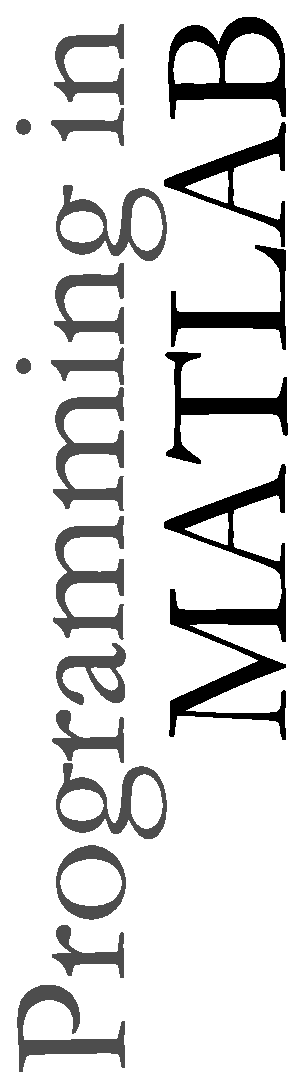
\includegraphics[width=0.75\textwidth]{./../eps/title-text}\\[1cm] 
\end{center}
\end{minipage}
\begin{minipage}{0.7\textwidth}
\begin{center}
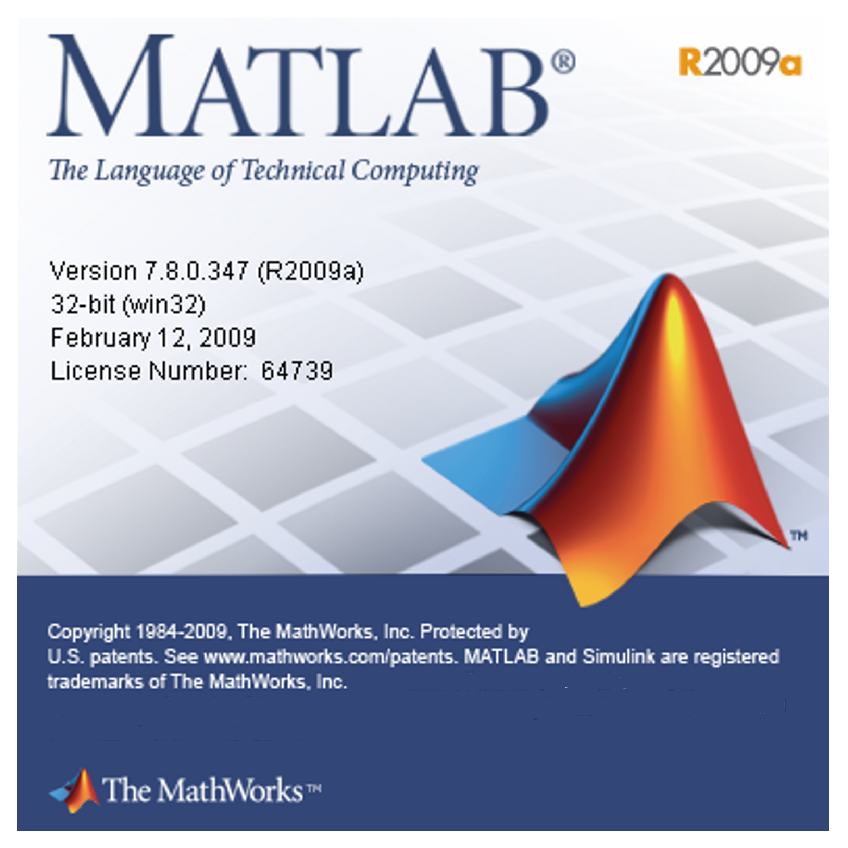
\includegraphics[width=0.75\textwidth]{./../eps/matlab-about}\\[1cm]
\end{center}
\vfill
\end{minipage}


\vspace{3em}
\begin{center}

\includegraphics[width=0.4\textwidth]{./../eps/logo}\\[1cm] 
{\small \today}
\end{center}
\vfill
\begin{minipage}{0.99\textwidth}
\begin{flushright} \large
Prof. Dr. Ir. \textsc{W.~Bouten}\\
\vspace{0.5em}
\textsc{Peter Kraal}\\
\vspace{0.5em}
\textsc{Jurriaan H. Spaaks}\\
\end{flushright}
\end{minipage}
 
\end{titlepage}

\insertemptypage{}

\tableofcontents
\newpage

\listofproject
\insertemptypage{}

\listoftables
\insertemptypage{}

\mainmatter
\chapter{Introduction}
\thispagestyle{fancy}

When you watch the weather forecast, all predictions are based on the results of computer models. With real-time input of meteorological conditions and a model that simulates (part of) the global climate system, it is possible to predict the weather for the near future. Of course these models can never be 100 percent accurate, as everybody who has gone out in shorts and ended up soaked with rain can confirm.

In another example of modeling, the United Nations use computer models to predict the development of global phenomena like diseases, famine and death. Other model simulations based on demographics and population data can be used to estimate future trends in world population and migration.

Science has made tremendous progress in the last decades. Measuring techniques, instruments and knowledge transfer are becoming better and more efficient. But the examples above show the importance of another factor: the increasing use of computers to analyze and generate data. It is now possible to quickly access, analyze and manipulate amounts of data on your computer that would have taken up complete libraries in the past. And the possibilities reach beyond simply using existing data: models can approximate real-life processes and generate data that was not available before. Furthermore, models can deepen the understanding of the earth and all of the processes influencing our environment.

The computer programs you may have so far encountered in your life - Microsoft Excel, Word and PowerPoint, ArcGIS and Stella - are all packages for specific tasks. Excel, ArcGIS and Stella allow you to analyze, manipulate and visualize data to some degree. However, you are always restricted to the features that the software developers included in these packages. 

Alternatively, programming languages, such as Fortran, Basic, C, C++, Pascal, Turbo Pascal, Object Pascal (Delphi), R, Python and \MATLAB{} give you the freedom to write your own programs that simulate and calculate almost anything you want them to. Many specific scientific problems cannot be tackled without a custom-made computer program. 

In this course you will use MATLAB, a `next-generation' programming language based on C and Fortran, but without all the programming overhead that comes with those languages, making MATLAB much easier to use in comparison.

At the University of Amsterdam the generation and transfer of programming knowledge has become an important feature of the educational program. It is the believe---and rightly so---that a student who is able to write his own computer programs, and understand those of others, has more flexibility when analyzing, manipulating and understanding data. With Excel you cannot realistically model global climate change or any other (complicated) earth process. At this moment, MATLAB is being used to model hydrological systems, erosion in the semi-arid Mediterranean, rockfall in the Alps, the interaction between soil and water, or bird migration from Scandinavia to Africa, to name but a few current research topics where programming is involved.

\MATLAB{}'s user-friendly interface and programming flexibility have made it a popular tool for scientists. On the Internet, large amounts of \MATLAB{} programs and tutorials can be found. Furthermore, MATLAB is an `array-oriented' programming language and therefore very suitable for spatial (1D, 2D, 3D, 4D\dots) calculations.

Because of all this, we think it is important that a student in Earth Sciences at the University of Amsterdam be introduced to \MATLAB{} at an early stage. This course, Programming in \MATLAB{}, has been developed to make you comfortable with programming in \MATLAB{} and teach you how the Earth's processes can be converted into \MATLAB{} programs.

\vspace{2em}

\noindent \textbf{Take your time going through the exercises. Make sure you try to interpret your results. If you rush too much, you won't be able to pick up the information and you will easily forget what you have learned. }



\chapter{Getting started}
\thispagestyle{fancy}
\label{ch:getting-started}

\begin{action}
Start \MATLAB{} by clicking \guitext{Start} \ding{217} \guitext{Programs} \ding{217} \guitext{MATLAB} \ding{217} \guitext{MATLAB~R2009a} and click on \guitext{MATLAB~R2009a}.
\end{action}
\begin{action}
Go to \guitext{Desktop} in the menu bar and select \guitext{Desktop Layout} and then choose \guitext{Command Window Only}.
\end{action}

\noindent The Command Window\index{Command Window} is the window where you type your commands at the `\verb#>>#'-sign, also known as `prompt'\index{prompt}. These commands are then being executed by \MATLAB{} after pressing the \guitext{Enter} key.

\section{Creating your own work directory}



To create your own work directory\index{work directory}, click the \guitext{Browse for Folder} button (see Figure \ref{fig:browse-for-folder}) located to the right of the \guitext{Current Directory} drop-down list on the \MATLAB{} button bar. This button is used to change or create your work directory. Click to create your work directory or to change the directory to the directory you will be working from. Now go to the \guitext{Desktop} menu and click a checkmark next to \guitext{Current Directory}. You will see that you are now in the directory you selected through using the \guitext{Browse for Folder} button.

\begin{figure}[!htbp]
  \centering
    \fbox{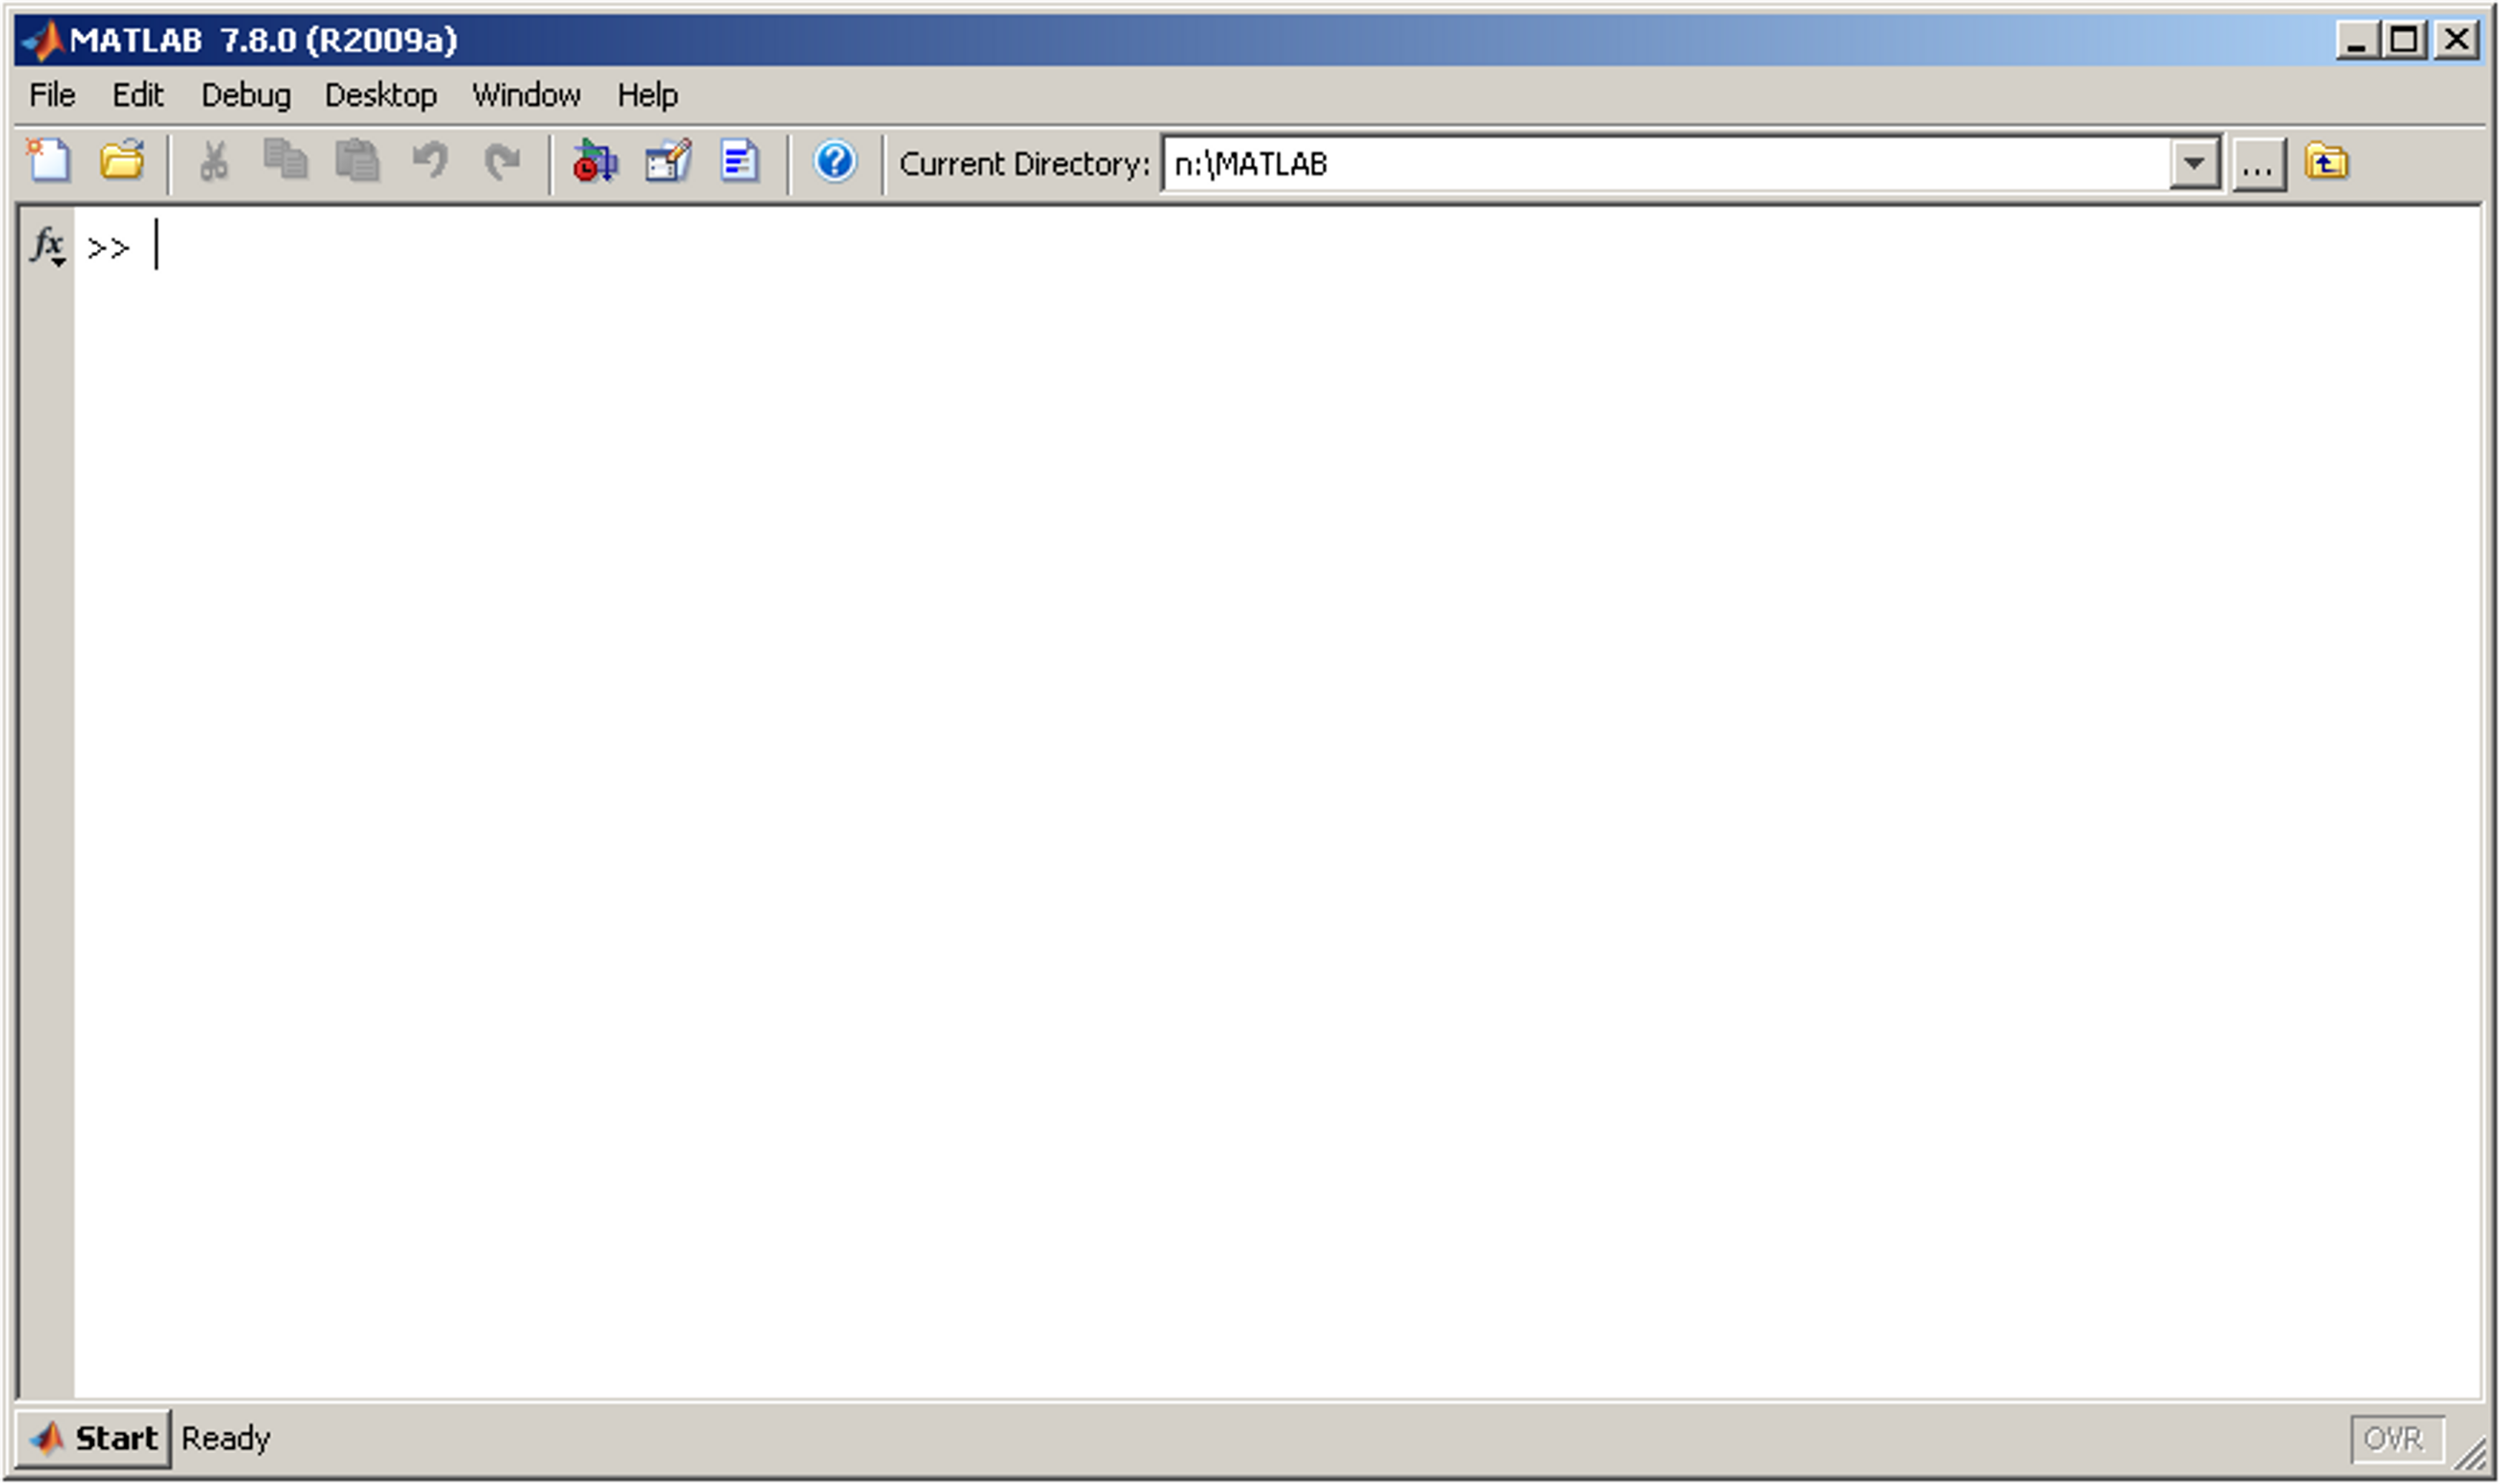
\includegraphics[width=1.0\textwidth]{./../eps/browse-for-folder}}
  \caption{Location of the ``browse for folder''-button.}\label{fig:browse-for-folder}
\end{figure}


\hintbox{Make it a habit to start every new exercise by selecting the appropriate directory for that exercise. Be sure that you are in that directory when executing your commands.}


\begin{action}
Type
\end{action}
\prompt{Groningen = 2.33}
\noindent and then press ``Enter'', keeping in mind that `{\tt \textgreater\textgreater}' is the command prompt. Note that the \MATLAB{} Command Window now displays the following output:
\begin{verbatim}
Groningen = 

    2.3300

\end{verbatim}
This output lets you know that \MATLAB{} has created a variable named \verb#Groningen# whose value is equal to \verb#2.3300#.

Go to the \guitext{Desktop} menu and click a checkmark next to \guitext{Workspace}, and you will see the \verb#Groningen# variable listed in the \MATLAB{} Workspace. Alternatively, you can type \verb#who#\index{who@\texttt{who}} or \verb#whos#\index{whos@\texttt{whos}} at the command prompt. These commands will list the variables in your Workspace in the Command Window.
\begin{action}
Type 
\end{action}
\prompt{Utrecht = 2.12}
\noindent and then press \guitext{Enter}.
\begin{action}
Type 
\end{action}
\prompt{Maastricht = 1.92}
\noindent and then press \guitext{Enter}. Both the \verb#Utrecht# and \verb#Maastricht# variables are now listed in the \MATLAB{} Workspace window.
\begin{action}
Calculate the mean of the total yearly precipitation for these three cities:
\end{action}
\prompt{Prec = (Groningen + Utrecht + Maastricht)*365/3}

\noindent Now, not only do \verb#Groningen#, \verb#Utrecht#, and \verb#Maastricht# appear in the workspace, but a new variable \verb#Prec# is also present. These short calculations are simple examples of the arithmetic operations that can be executed in \MATLAB{}. Table~\ref{tab:operations} gives an overview of the basic mathematic operators used in \MATLAB{}.
\begin{table}[t]
\caption{\MATLAB{} operations.}
\label{tab:operations}
\vspace{-0.5em}
\centering
\begin{tabular}{|l|l|l|}
\hline
\textbf{Operation}&\textbf{Symbol}&\textbf{Example}\\
\hline
Addition\index{addition}&\verb#+#&\verb#5+6.7#\\
\hline
Subtraction\index{subtraction}&\verb#-#&\verb#8.63-5.24#\\
\hline
Multiplication\index{multiplication}& \verb#*#&\verb#3*2#\\
\hline
Division\index{division}& \verb#/#&\verb#1/4#\\
\hline
Exponentiation\index{exponentiation}& \verb#^#&\verb#3^2#\\
\hline
\end{tabular}
\end{table}
Note: The square root is merely an instance of the Exponentiation notation:  \verb#A^0.5#$\equiv$\verb#sqrt(A)#\index{sqrt@\texttt{sqrt}}.

\begin{action}
Clear the workspace using the command \verb#clear#\index{clear@\texttt{clear}}
\end{action}
\begin{action}
Assign the value 1 to the variable \verb#ExampleVar#:
\end{action} 
\prompt{ExampleVar = 1}
\begin{action}
Assign the value 14 to the variable \verb#EXAMPLEVAR#:
\end{action}
\prompt{EXAMPLEVAR = 14}
\begin{action}
Check the workspace by typing:\\
\end{action}
\prompt{whos}
\noindent and then pressing the \guitext{Enter} key.
\begin{verbatim}
  Name             Size                   Bytes  Class          Attributes

  EXAMPLEVAR       1x1                        8  double array
  ExampleVar       1x1                        8  double array

\end{verbatim}
This procedure is meant to demonstrate that \MATLAB{} is case-sensitive\index{case-sensitive}: \verb#EXAMPLEVAR# and \verb#ExampleVar# are two different variables. Another way to check structures of variables entered into the \MATLAB{} Workspace is to double-click the variable in the \MATLAB{} \guitext{Workspace} window. This opens the variable up in the array editor. Check the value of the variable \verb#EXAMPLEVAR# by double-clicking its variable in the \guitext{Workspace} window.
\begin{action}
Check the value of the variable \verb#EXAMPLEVAR#.
\end{action}


\hintbox{\label{tip:naming-conventions}Be aware that as we work through the manual, the use of any special text characters (such as {\tt*}, {\tt\&}, {\tt\MVAt}, {\tt\#}, and {\tt?} ) within variable names is prohibited, the exception being the underscore `{\tt\_}' character. This is because these characters often have special effects on operations. Variable names can contain up to 31 characters, but must start with a letter followed by any combination of letters, digits or underscores.}

\begin{action}
Now, go to the \guitext{Desktop} menu and click a checkmark next to \guitext{Command History}. This opens a new window within the \MATLAB{} Graphical User Interface\index{Graphical User Interface} (GUI\index{GUI}) listing the commands that you have entered in the \guitext{Command Window}. Figure \ref{fig:gui} shows you what your GUI should look like now. 
\end{action}


\begin{figure}[!ht]
  \centering
    \fbox{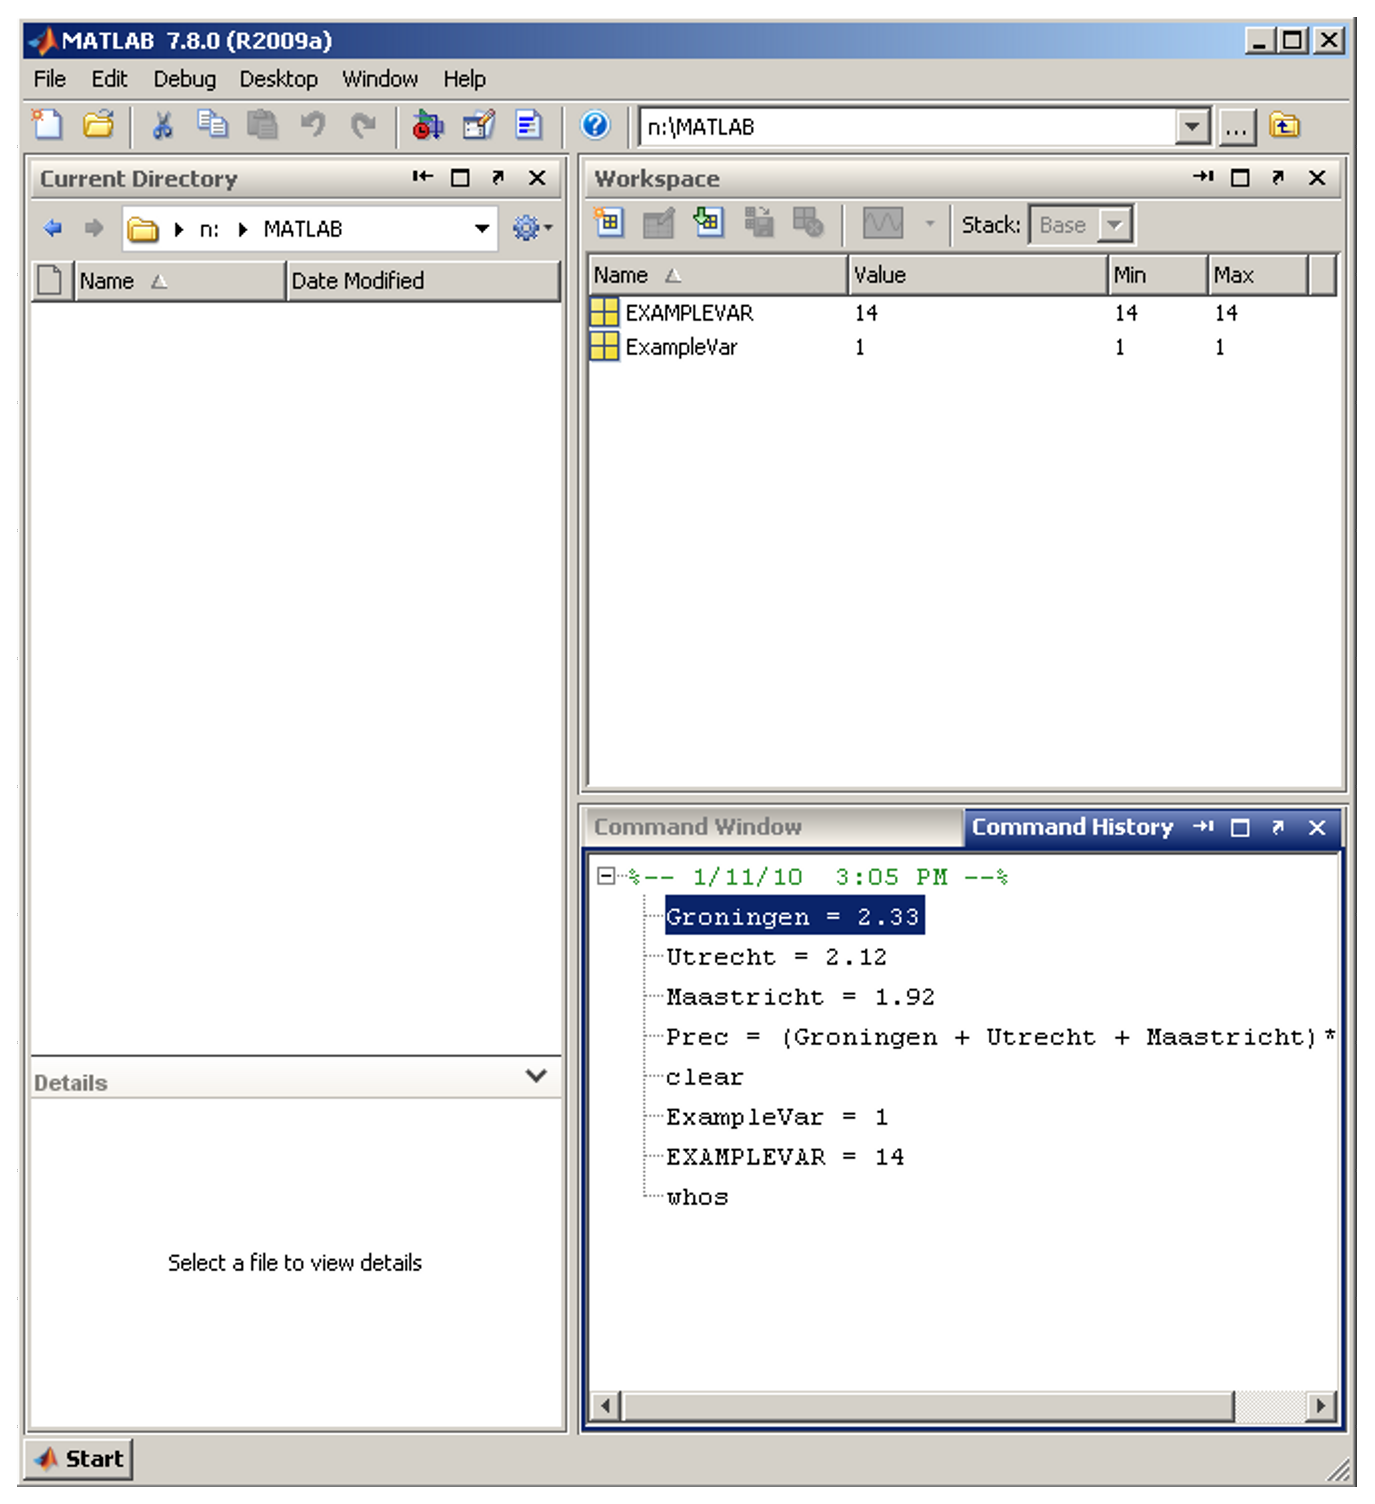
\includegraphics[width=0.9\textwidth]{./../eps/gui.eps}}
  \caption{\MATLAB{} Graphical User Interface (GUI). Note that the Command Window and Command History are docked into the same panel. You can change the layout of your GUI by clicking the title bar of the panel that you want to put somewhere else, and moving the mouse pointer while holding down the left mouse button.}\label{fig:gui}

\end{figure}


\hintbox{\MATLAB{} remembers the commands that have been typed at the prompt. You can use the up and down arrows to select any previously typed commands. You can also check the \guitext{Command History} item in the \guitext{Desktop} menu.}



\chapter{Arrays: scalars, vectors and matrices}
\thispagestyle{fancy}
\label{ch:arrays}

Besides using \MATLAB{} as a common calculator, it is possible to perform calculations on entire datasets. These variables must be stored in the workspace and addressed by their variable name. Variables are stored in the \MATLAB{} workspace as arrays. The four main array types that we will use are:



\begin{description}
\item [Scalar\index{scalar}] 1x1 array containing one value
\item [Vector\index{vector}] a row or column array (1xM or Mx1 array) containing M values
\item [Matrix\index{matrix}] a 2-dimensional array (e.g. a map)
\item [Multi-dimensional arrays\index{multi-dimensional arrays}] e.g. a 5x2x3 array containing 30 values
\end{description}

\hintbox{You can retrieve the size of an array by issuing a {\tt size(X)}\index{size@\texttt{size}} command, where {\tt X} represents the array that you want to know the size of.}



\section{Data types\index{data types} and array classes\index{array classes}}

\MATLAB{} arrays can contain three different data types: integer\index{integer}, floating point\index{floating point}, and character\index{character} data. 

\hintbox{A character variable is often referred to as a `string'\index{string}, especially when it contains more than one character.}

\noindent A description of different data types and the array classes in which they are stored is given in Table~\ref{tab:array-classes}.

\begin{table}[ht]
\caption{Array classes}
\label{tab:array-classes}
\vspace{-0.5em}
\centering
\begin{tabular}{|p{2cm}|l|p{3cm}|p{2cm}|}
\hline
\textbf{Data type}&\textbf{Examples}&\textbf{Description}&\textbf{Array class}\\
\hline
Integer&\verb#-2 -5 -8 0 2 34 221#&(+/-) Whole numbers&Double array\\
\hline
Floating point&\verb#3.2232 �8.323 5823.22#& (+/-) Fractional numbers&Double array\\
\hline
Character&\verb#y L \ = ] - K , u ;#&ASCII text characters&Character array\\
\hline
\end{tabular}
\end{table}



\section{Creating arrays}

Besides using existing datasets for analysis, it is important to be able to create and manipulate your own arrays within the \MATLAB{} environment. This can vary from creating a simple vector with an increasing value from 1 to 365 to serve as a time indicator for a certain process to complex 4-D arrays with certain parameters at a place in space (X, Y, Z) that change over time. The value of each position in an array can then be manipulated to simulate a process. These operations can be performed on complete arrays or selected cells.

 
\begin{action}
Type 
\end{action}
\prompt{A = [1,2,3;4,5,6]}
\noindent \verb#A# is now present in the workspace as a 2x3 double array. When declaring arrays other than scalars, the array contents must be in brackets \verb#[ ]#. If you take a closer look at the output that \MATLAB{} returns, you'll see that you just made an array with 2 rows and 3 columns. 
\hintbox{Commas ({\tt,}) serve as column delimiters, and semicolons ({\tt;}) are row delimiters.}
\noindent There are several ways to create vectors:
\begin{action}
Type 
\end{action}
\prompt{k = [1:1:9]}
\noindent press \guitext{Enter} and interpret the result.

\begin{action}
Type 
\end{action}
\prompt{m = [21:-2:13]}
\noindent press \guitext{Enter} and interpret the result. As you can see, the syntax of this command is \verb#[#minimum\verb#:#increment\verb#:#maximum\verb#]#.

\begin{action}
Generate an array starting with 10.2, decreasing with 0.3 and ending at 6.0.
\end{action}

\begin{action}
As simple as you can generate 1-D arrays, you can also make 2-D arrays; type 
\end{action}
\prompt{F = [-10:1:10;40:-1:20]}
\noindent and interpret the result.


\begin{action}
Type 
\prompt{G = [-5:1:15;8:-0.5:1.0]}
\noindent and interpret the error.
\end{action}
\begin{action}
Once an array contains one of the three data types, it cannot contain another data type as well. Type 
\end{action}
\prompt{H = [1,2,3;\squote{PiM}]}
\noindent and interpret the result.

 
\begin{action}
Now type 
\end{action}
\prompt{I = [1,2,3,4;\squote{PiM}]}
\noindent and interpret the error.

\section{Manipulating arrays by their subscripts\index{subscripts} and indices\index{index}\index{indices}}

Elements of arrays are identified by their positions in the array. So\dots
\vspace{0.5em}
\prompt{F(2,6)}
\noindent returns 35. This is the value of the element in the second row and the sixth column in matrix \verb#F#. 

Elements can also be identified by their index. The index is a counter that starts at the first row and first column, then continues down in the first column and then takes next column. To clarify the difference between indices and subscripts, take a closer look at the tables below:



\begin{table}[ht]
\caption{Array elements identified by subscripts}
\label{tab:subscripts}
\vspace{-0.5em}
\centering
\begin{tabular}{|p{0.75cm}|p{0.75cm}|p{0.75cm}|}
\hline
(1,1)&(1,2)&(1,3)\\
\hline
(2,1)&(2,2)&(2,3)\\
\hline
(3,1)&(3,2)&(3,3)\\
\hline
\end{tabular}
\end{table}

\begin{table}[ht]
\caption{Array elements identified by indices}
\label{tab:indices}
\vspace{-0.5em}
\centering
\begin{tabular}{|p{0.75cm}|p{0.75cm}|p{0.75cm}|}
\hline
(1)&(4)&(7)\\
\hline
(2)&(5)&(8)\\
\hline
(3)&(6)&(9)\\
\hline
\end{tabular}
\end{table}


\begin{action}
Retrieve the value of the element denoted by subscript 2,1 in matrix {\tt A}. What value do you expect?
\prompt{A(2,1)}
\end{action}

\hintbox{Parenthesis symbols {\tt( )} are used to point to elements of an array, in contrast to the {\tt[ ]} square brackets that are used to assign values to the array.}

\begin{action}
What is the index of the value 23 in the matrix {\tt F}? And what are the subscripts?
\end{action}

\begin{action}
Alter the values in a matrix by calling their indices or subscripts and assigning a new value: 
\end{action}
\prompt{F(20) = -40}
\noindent Now check what has changed in the matrix {\tt F}.

\vspace{1em}
\noindent You have now altered one array element of matrix {\tt F} by using a scalar as index. You can also change more than one array element of {\tt F}, at the same time, by using an index vector instead of just one index scalar. 

\begin{action}
Carefully interpret the sentence above and (try to) change the array elements of {\tt F} to �50 where the index is equal to one of the elements of the vector {\tt IndVec}, when given: 
\end{action}
\prompt{IndVec = [3,15,2,8,19]}

\begin{action}
Can you this do this in a single command? 
\end{action}
 

\section{Matlab demonstrations}

Maybe this is a good moment to take a break for a while and to have a look at some demonstrations for 10--15 minutes, as \MATLAB{} has an extensive `{\tt demo}'\index{demo@\texttt{demo}} function. When you see what you can do with \MATLAB{}, you have a better reference while studying this text and while doing the exercises. Select one or two of the most instructive demos and share these with your neighbors. 

\begin{action}
Start \MATLAB{} demonstrations by typing {\tt demo} on the \MATLAB{} command line. 
\end{action}

\noindent The help documentation window that pops up consists of two panes. Read the contents of the right pane. After that, try expanding one of the menu tree items in the left pane, for example \MATLAB{} \ding{217} graphics (see Figure~\ref{fig:demo}).

\begin{figure}[!ht]
  \centering
    \fbox{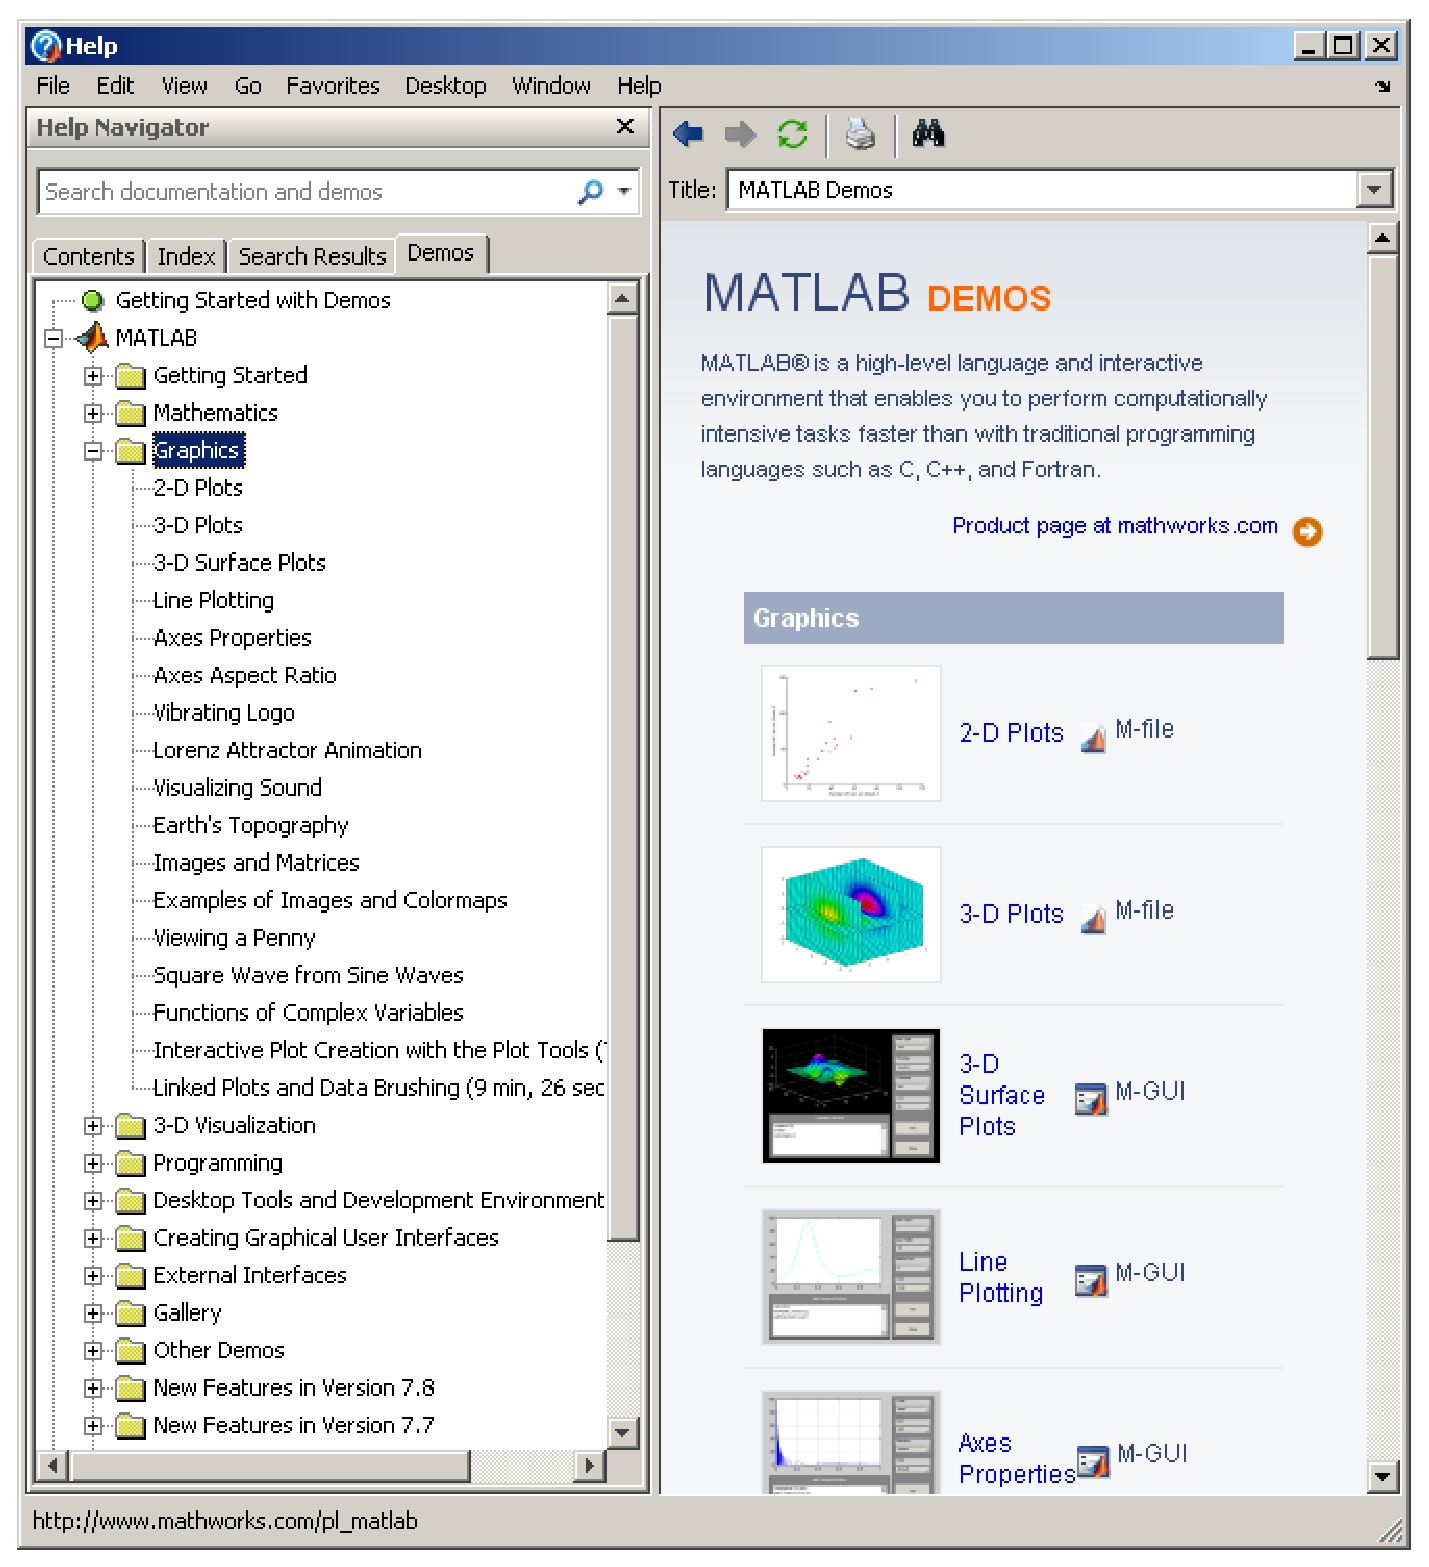
\includegraphics[width=1.0\textwidth]{./../eps/demo.eps}}
  \caption{\MATLAB{} demonstrations.}
  \label{fig:demo}
\end{figure}



\section{Arithmetic operations on matrices and vectors}

Just as you can perform calculations on scalars (as we did in the exercise with the precipitation), you could perform calculations on larger arrays as well. Some examples are outlined below:

\subsection{Multiplication of a scalar with a 2-D array}

\begin{equation}
\label{eq:scalar-matrix-multiplication}
5\ast
\left[ 
\begin{array}{rrr}
4&5&2\\
1&9&0\\
1&5&5\\
\end{array}
\right]
=
\left[
\begin{array}{rrr}
20&25&10\\
5&45&0\\
5&25&25\\
\end{array}
\right]
\end{equation}

\noindent Or, in \MATLAB{}:
\prompt{A = 5}
\prompt{B = [4,5,2;1,9,0;1,5,5]}
\prompt{C = A * B}


\subsection{Addition of 2-D arrays}


\begin{equation}
\label{eq:addition-2D}
\left[ 
\begin{array}{rrr}
-1&2&0\\
2&-3&1\\
-4&0&5\\
\end{array}
\right]
+
\left[ 
\begin{array}{rrr}
4&5&2\\
1&9&0\\
1&5&5\\
\end{array}
\right]
=
\left[
\begin{array}{rrr}
3&7&2\\
3&6&1\\
-3&5&10\\
\end{array}
\right]
\end{equation}


\noindent Or, in \MATLAB{}:
\prompt{D = [-1,2,0;2,-3,1;-4,0,5]}
\prompt{B = [4,5,2;1,9,0;1,5,5]}
\prompt{E = D + B}


\subsection{Multiplication of 2-D arrays (`dot-product')}


\begin{equation}
\label{eq:multiplication-2D-dot-product}
\left[ 
\begin{array}{rrr}
3&1&7\\
8&4&6\\
\end{array}
\right]
\bullet
\left[ 
\begin{array}{rrr}
4&5\\
2&1\\
9&0\\
\end{array}
\right]
=
\left[
\begin{array}{rrr}
77&16\\
94&44\\
\end{array}
\right]
\end{equation}


\noindent Or, in \MATLAB{}:
\prompt{F = [3,1,7;8,4,6]}
\prompt{G = [4,5;2,1;9,0]}
\prompt{H = F * G}

\noindent In general, elements of \verb#H# are calculated using:
\begin{equation}
\label{eq:matrix-multiplication}
H(r,c) = \sum_{k=1}^{nElems}{F(r,k)\times{}G(k,c)}
\end{equation}
in which $r$ is the row number, $c$ is the column number, $nElems$ is the number of columns in $F$ (or, equivalently, the number of rows in $G$). For example:

\noindent \begin{array}{cccccccccccccl}
H(1,1)& = &F(1,1)&*&G(1,1)&+&F(1,2)&*&G(2,1)&+&F(1,3)&*&G(3,1)&=\\ 
&&3&*&4&+&1&*&2&+&7&*&9&=77\\ 
\end{array}

\noindent Note that \verb#F * G# returns a different result than \verb#G * F#.

\subsection{Multiplication of 2-D arrays (element-by-element)}

\begin{equation}
\label{eq:multiplication-2D-product}
\left[ 
\begin{array}{rrr}
3&1&7\\
8&4&6\\
5&3&4\\
\end{array}
\right]
\ast
\left[ 
\begin{array}{rrr}
4&5&2\\
1&9&0\\
1&5&5\\
\end{array}
\right]
=
\left[
\begin{array}{rrr}
12&5&14\\
8&36&0\\
5&15&20\\
\end{array}
\right]
\end{equation}

\noindent In \MATLAB{}, if you want to calculate the product of \verb#A# and \verb#B# element-by-element, you need to use a period sign (`\verb#.#') between the first matrix and the operator:

\prompt{J = [3,1,7;8,4,6;5,3,4]}
\prompt{B = [4,5,2;1,9,0;1,5,5]}
\prompt{K = J .* B}
\noindent so that elements of K are calculated using $K(r,c) = J(r,c)*B(r,c)$. Note that there is no difference between $J * B$ and $B * J$, since the array elements are multiplied on an element-by-element basis anyway.

\begin{action}
Is it possible to calculate \verb#M*N# if both \verb#M# and \verb#N# are arrays of size 3x2? Why or why not? If you don't know, just try it out in the Command Window! 
\end{action}
\begin{action}
Same question for \verb#M.*N#
\end{action}


\vspace{2em}

\noindent Recall the precipitation example in Chapter \ref{ch:getting-started}. In that example, the precipitation had been measured for a different period in each city:
\begin{table}[ht]
\caption{Precipitation records}
\label{tab:precipitation-records}
\vspace{-0.5em}
\centering
\begin{tabular}{|l|l|l|}
\hline
\textbf{City}&\textbf{Period}&\textbf{Mean Daily Precipitation}\\
\hline
Groningen&12&2.33\\
\hline
Utrecht&27&2.12\\
\hline
Maastricht&18&1.92\\
\hline
\end{tabular}
\end{table}



\begin{action}
Create two 3x1 arrays, \verb#Period# and \verb#MDP# (Mean Daily Precipitation), that contain the measuring period (in days) and mean daily precipitation (in mm/day), respectively for the three Dutch cities. Use matrix operations to calculate a 3x1 array \verb#TP# with total precipitation (in mm) for every city during their respective measuring periods.
\end{action}



\section{Concatenation}
\label{ch:concatenation}
It can be useful to combine separate arrays with related data into one array. This is called concatenation\index{concatenation}.

\begin{action}
Type:
\end{action}
\prompt{A = 5}
\prompt{B = 6}
\prompt{C = [A,B]}
\noindent and check what \verb#C# contains.

\begin{action}
What is the difference between typing \verb#C = [A;B]# instead of \verb#C = [A,B]#?
\end{action}

\begin{action}
It is also possible to add a new row and/or column to an existing array:
\end{action}
\prompt{D = 1}
\prompt{E = 3}
\prompt{F = 4}
\prompt{G = [D,2;E,F;C]}


\begin{action}
Concatenate the three arrays \verb#Period#, \verb#MDP#, and \verb#TP# into one array named \verb#PrecInfo#.
\end{action}


\begin{action}
Take 15 minutes to review what you have learned so far in chapters \ref{ch:getting-started} and \ref{ch:arrays}.
\end{action}

\project{Columbia River}
\label{pr:columbia}
\noindent In this exercise you will use much more data than can be typed quickly, so you will load the data from a file. You also cannot display all results as numbers on the screen, so you will learn some of the basics of making graphical presentations.

Suppose that you have measured the stream water velocity in the Columbia River. This data is stored in a file titled `columbia\_river.mat'.

\begin{action}
Go to \url{http://blackboard.ic.uva.nl} and download the file \mbox{`pim\_files.zip'}. This zipfile contains all the files that you will need during this course. Unzip it to your network drive or usb-memory. It contains the folder structure displayed in Figure~\ref{fig:folder-structure}. As you can see, each chapter has its own folder. Some folders contain subfolders labeled according to the project number.
\end{action}

\begin{figure}[!ht]
  \centering
    \fbox{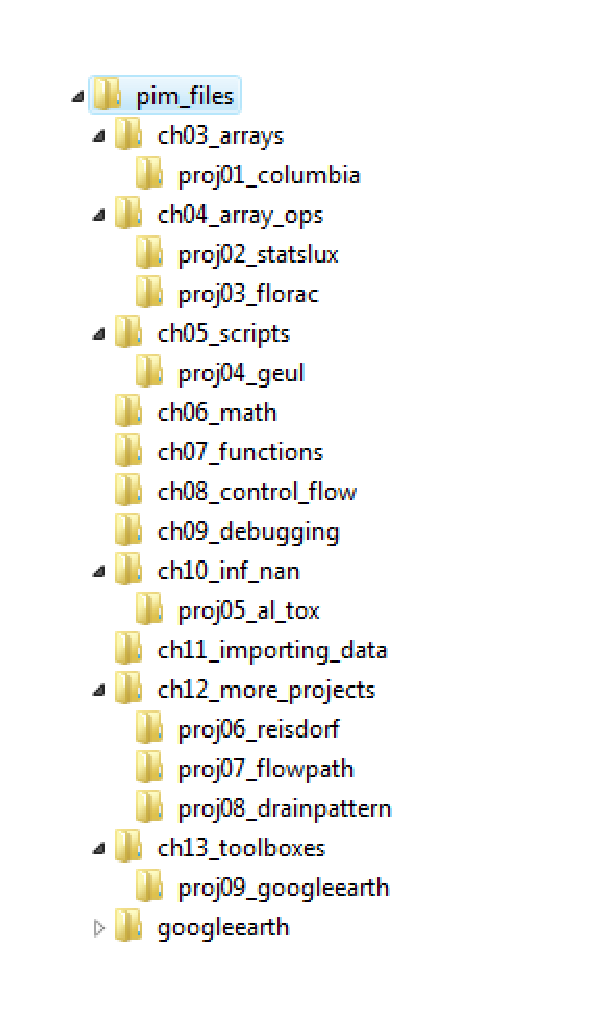
\includegraphics[width=0.33\textwidth]{./../eps/folder-structure}}
  \caption{Folder structure.}
  \label{fig:folder-structure}
\end{figure}



\begin{action}
Set your work directory to `\textbackslash{}ch03\_arrays\textbackslash{}proj01\_columbia'. The file `columbia\_river.mat' contains stream velocity data from the Columbia River in Oregon, averaged over total depth\footnote{Data from Savini and Bodhaine (1971) US Geological Survey}.
\end{action}

\hintbox{Make it a habit to clear your workspace with the {\tt clear} command before you start a new exercise. Doing this makes your calculations faster and will help diminish the interference from unnecessary variables. 
}

\begin{action}
Load \mbox{`columbia\_river.mat'} into the workspace (a *.mat file is a binary file, it can contain multiple variables):
\end{action}
\prompt{load columbia\_river.mat}\index{load@\texttt{load}}


\begin{action}
Check the variables you loaded for Columbia River in the workspace. Check the size and the values for these arrays in the \guitext{Workspace} window.
\end{action}


\hintbox{A calculation statement that does not end with a semicolon ( {\tt ;} ) echoes the answer to the screen. This may be undesirable if you are working with large matrices, because you don't want these matrices scrolling endlessly on your screen. A statement with a semicolon carries out the same task but does not echo the result to the screen. Display the array {\tt Sensor\_1} from the Columbia River project and then again using the semicolon:
\vspace{0.25em}
 
\prompt{Sensor\_1}
\prompt{Sensor\_1;}

}%close hintbox

\section{Simple plotting}
\noindent \MATLAB{} can display all kinds of graphs. An easy-to-use visualization tool is the \verb#plot(X,Y)#\index{plot@\texttt{plot}} command. This command plots the elements of a vector \verb#X# on the x-axis versus the values of a vector \verb#Y# on the y-axis (see Figure~\ref{fig:plotxy}).




\begin{figure}[ht]
\begin{minipage}{0.65\textwidth}
\centering
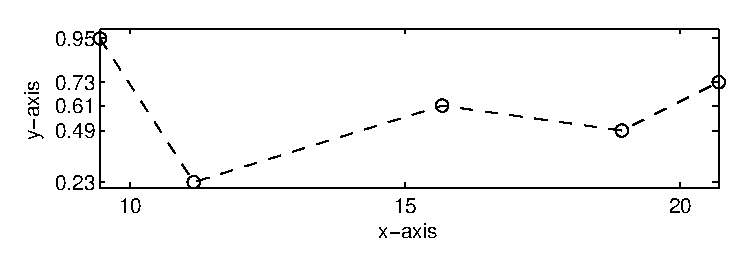
\includegraphics[width=\textwidth]{./../eps/plotxy}
\end{minipage}
~\hfill~
\begin{minipage}{0.25\textwidth}
\centering
\begin{tabular}{|c|c|}
\hline
\textbf{X}&\textbf{Y}\\
\hline
9.46&0.95\\
11.17&0.23\\
15.69&0.61\\
18.95&0.49\\
20.71&0.73\\
\hline
\end{tabular}
\end{minipage}
\caption{{\tt plot} with X and Y coordinates specified.}
\label{fig:plotxy}
\end{figure}



If no X-vector is specified (\verb#plot(Y)#), \MATLAB{} visualizes the data from vector \verb#Y# versus its indexes (see Figure~\ref{fig:ploty} on page \pageref{fig:ploty}).



\begin{figure}[ht]
\begin{minipage}{0.65\textwidth}
\centering
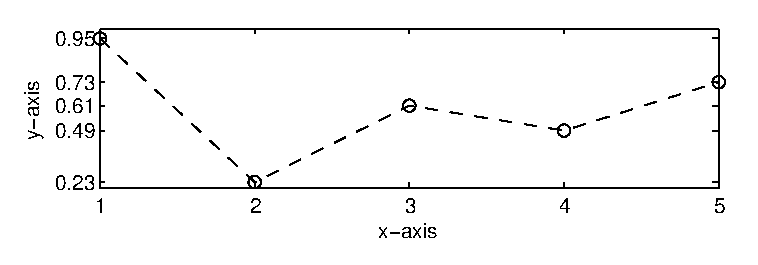
\includegraphics[width=\textwidth]{./../eps/ploty}
\end{minipage}
~\hfill~
\begin{minipage}{0.25\textwidth}
\centering
\begin{tabular}{|c|c|}
\hline
\textbf{X}&\textbf{Y}\\
\hline
1&0.95\\
2&0.23\\
3&0.61\\
4&0.49\\
5&0.73\\
\hline
\end{tabular}
\end{minipage}
\caption{{\tt plot} with only Y coordinates specified explicitly.}
\label{fig:ploty}
\end{figure}

\begin{action}
Display the data of \verb#Sensor_1# using the plot command.
\end{action}
\prompt{plot(Sensor\_1)}


\noindent This plot contains the time on the horizontal axis and the stream water velocity on the vertical axis. To indicate what the figure you created is about, we need to give it a title. This is done using the {\tt title(\squote{s})}\index{title@\texttt{title}} command. The variable \verb#s# represents the text to be used in the title. Don't forget to put this text string inside single quotation marks, otherwise \MATLAB{} will return an error. 

\begin{action}
Give the figure a title: `Columbia River, near Priest River Dam'. If you are not sure how to assign titles to figures, you can consult the \verb#doc#\index{doc@\texttt{doc}} function (see the tip below). 
\end{action}


\noindent Just as we can put a title on a figure, it's also possible to assign text labels to the axes. This is done using the commands {\tt xlabel}\index{xlabel@\texttt{xlabel}} and {\tt ylabel}\index{ylabel@\texttt{ylabel}}.

\hintbox{There are different ways to get help in \MATLAB{}. By far the most important and easy-to-use is the {\tt doc} command. For instance try typing {\tt doc mean} to read about how to use \MATLAB{}'s built-in function to calculate the mean of an array. Other commands that are sometimes helpful are: {\tt help}\index{help@\texttt{help}} and {\tt lookfor}\index{lookfor@\texttt{lookfor}}.}


\begin{action}
Consult the \verb#doc# function to find out how to assign labels to the x and y axes. Label the x-axis `Time (minutes)' and the y-axis `Velocity (m/s)'.
\end{action}

\begin{action}
Type 
\end{action}
\prompt{legend(\squote{velocity [m/s]})}\index{legend@\texttt{legend}}
\noindent to create a legend for the stream velocity plot of the Columbia River.

\vspace{1em}
\noindent There is a problem: previous experience with this sensor shows that a stream velocity correction is needed for this stream segment: 

\begin{equation}
TV1 = -0.18 + 0.987 * MV1 
\end{equation}
where $TV1$ is the true stream velocity and $MV1$ is the velocity as recorded by sensor~1.

\begin{action}
Calculate the true stream velocity of the river, measured with sensor~1.
\end{action}

\noindent After 66 measurements, unfortunately sensor~1 broke down. Luckily, a backup sensor, sensor~2, was available at the same stream location. The variable \verb#Sensor_2# contains the data from this sensor. However, this one also needs a correction: 
\begin{equation}
TV2 = -0.02 + 1.002 * MV2
\end{equation}
where $TV2$ is the true stream velocity and $MV2$ is the velocity as recorded by sensor~2.


\begin{action}
Correct the second data set (\verb#Sensor_2#) with this algorithm and append the corrected sensor~2 data to the first 66 measurements gathered at sensor~1 into a new merged stream data array, called \verb#Columbia#. Plot the result. Try to plot the 2~variables \verb#Sensor_1# and \verb#Sensor_2# with different colors. Consult the help documentation if necessary.
\end{action}

\begin{action}
Print the figure you created for your Columbia River stream velocities.
\end{action}

\begin{action}
Save the merged and corrected data array into a binary file by typing:
\end{action}
\prompt{save merged\_sensors.mat Columbia}\index{save@\texttt{save}}
\noindent which means: save the content of the variable Columbia in the binary file `merged\_sensors.mat'.

\projectfooter{}



 % plot: add time vector to data.
\chapter{Array operations}
\thispagestyle{fancy}
\label{ch:array-ops}

\index{array operations}

\MATLAB{} has many possibilities for array operations. In this chapter, we will look at a few of them.

\section{Creating special \MATLAB{} arrays using utility matrices}

Up to this point, you created all matrices by manually filling rows and columns with values. Below are some of the \MATLAB{} utility functions that are `shortcuts' to special matrix formats: 



\begin{table}[ht]
\caption{\MATLAB{} utility matrices\index{utility matrices}}
\label{tab:utility-matrices}
\vspace{-0.5em}
\centering
\begin{tabular}{|p{4cm}|p{8cm}|}
\hline
\textbf{Function}&\textbf{Description}\\
\hline
{\tt zeros(M,N)}\index{zeros@\texttt{zeros}}&Generate an array of size MxN filled with zeros\\
\hline
{\tt ones(M,N)}\index{ones@\texttt{ones}}&Generate an array of size MxN filled with ones\\
\hline
{\tt rand(M,N)}\index{rand@\texttt{rand}}&Generate an array of size MxN filled with values that are randomly chosen from a uniform distribution between 0 and 1 \\
\hline
{\tt randn(M,N)}\index{randn@\texttt{randn}}&Generate an array of size MxN filled with values that are randomly chosen from a normal distribution with mean 0 and standard deviation 1\\
\hline
{\tt eye(M)}\index{eye@\texttt{eye}}&Generate an identity matrix of size MxM with ones on the diagonal and zeros on all other positions\\
\hline
\end{tabular}
\end{table}

\noindent For instance, {\tt A = [1,1,1;1,1,1]} has the same result as {\tt A = ones(2,3)}.

\vspace{1.5em}

\begin{action}
Clear your workspace and type
\prompt{J = rand(7,5)}
\noindent and interpret the result. If necessary use the documentation by typing: 
\prompt{doc rand}
\end{action}

\begin{action}
\noindent To extract a submatrix from {\tt J}, type:
\prompt{Jsub1 = J(6:7,:)}
\noindent and interpret the result.
\end{action}

\noindent Since in this case no column numbers are specified, \textbf{all} values of {\tt J} that are on the 6$^{th}$ or 7$^{th}$ row of {\tt J} are selected.

\begin{action}
Now try to extract {\tt Jsub2}, a 7x2 array containing the last two columns of {\tt J}.
\end{action}

\begin{action}
Create a 4x5 matrix filled with only 7s
\end{action}

\begin{action}
Create a 4x4 matrix filled with -1 but with 2 on the diagonal
\end{action}

\begin{action}
Create a matrix with 3 columns and 7 rows filled with uniform random numbers between �3 and -1
\end{action}

\section{More MATLAB utility matrices}

\begin{action}
Type 
\end{action}
\prompt{G = [1,2;3,4;5,6]}


\begin{action}
Type
\end{action}
\prompt{Gflipped = flipud(G)}\index{flipud@\texttt{flipud}}
\noindent and interpret the result.

\begin{action}
Try the following \MATLAB{} functions as well: {\tt fliplr}\index{fliplr@\texttt{fliplr}} and {\tt rot90}\index{rot90@\texttt{rot90}}. Describe what happens to the array for each command. Again use {\tt doc} to get more insight in the possibilities of these functions.
\end{action}
\begin{action}
Type
\end{action} 
\prompt{Gtran = transpose(G)}\index{transpose@\texttt{transpose}}
\noindent Compare the original array {\tt G} and {\tt Gtran}. Describe the changes. 

\noindent (Note that 
{\tt \textgreater\textgreater\ Gtran = G\textquotesingle }\index{`@\texttt{\textquotesingle}}
has the same effect as {\tt \textgreater\textgreater\ Gtran = transpose(G)}).


 
\begin{action}
Create these three arrays:
\begin{itemize}
\item 2x3 array {\tt [6,7,8;2,3,4]}
\item 1x3 array {\tt [1,5,9]}
\item 1x3 array {\tt [10,11,12]}
\end{itemize}
Use concatenation and manipulation commands to compose this 3x4 array from the matrices you just created:
\end{action}
\begin{equation}
\left[
\begin{array}{cccc}
1&2&3&4\\
5&6&7&8\\
9&10&11&12\\
\end{array}
\right]
\end{equation}


\section{Statistical functions}
\MATLAB{} has a lot of built-in functions for statistical analysis of data sets. For example
{\tt min(M)} returns the minimum of a vector {\tt M}. 

\begin{action}
Clear the workspace
\end{action}

\begin{action}
Create a 2 x 6 array {\tt D} using: 
\prompt{D = [11:-3:-4;linspace(1,11,6)]}\index{linspace@\texttt{linspace}}
\end{action}

\begin{action}
Typing 
\prompt{min(D)}\index{min@\texttt{min}}
\noindent at the prompt will return:
\begin{verbatim}

ans =

     1     3     5     2    -1    -4

\end{verbatim}
Interpret how these numbers were determined.
\end{action}


\hintbox{{\tt ans}\index{ans@\texttt{ans}} (short for `answer') is a temporary variable name that \MATLAB{} automatically generates when the user does not specify a variable name. It is overwritten every time a variable name is not specified.}


\begin{table}[ht]
\caption{\MATLAB{} Statistical functions}
\label{tab:statistical-functions}
\vspace{-0.5em}
\centering
\begin{tabular}{|p{4cm}|p{8cm}|}
\hline
\textbf{Function}&\textbf{Description}\\
\hline
{\tt min(M)}& Calculates the minimum of a vector {\tt M}\\
\hline
{\tt max(M)}\index{max@\texttt{max}}& Calculates the maximum of a vector {\tt M}\\
\hline
{\tt mean(M)}\index{mean@\texttt{mean}}& Calculates the mean of a vector {\tt M}\\
\hline
{\tt median(M)}\index{median@\texttt{median}}& Calculates the median of a vector {\tt M}\\
\hline
{\tt sum(M)}\index{sum@\texttt{sum}}& Calculates the sum of a vector {\tt M}\\
\hline
{\tt std(M)}\index{std@\texttt{std}}& Calculates the standard deviation of a vector {\tt M}\\
\hline
{\tt prod(M)}\index{prod@\texttt{prod}}& Calculates the product of a vector {\tt M}\\
\hline
\end{tabular}
\end{table}


\noindent If {\tt M} is an array with {\tt R} rows and {\tt C} columns, {\tt sum(M)} returns a row vector. The n$^{th}$ element of this vector contains the sum of the n$^{th}$ element from all rows of {\tt M}. In other words, {\tt sum(M)} returns the sum of M, calculated over the first dimension, i.e. the rows. If you want to sum columns instead of rows, you can specify that the summation should be applied to the 2$^{nd}$ dimension (i.e. the columns) by:

\prompt{SumM = sum(M,2)}
\noindent The second argument to the function {\tt sum} is equal to 1 for operations on rows and 2 for operations on columns if {\tt M} is a 2-dimensional array, but can be higher if {\tt M} has more than 2 dimensions.


\begin{action}
If {\tt X = [0,1,2;3,4,5]}, calculate {\tt sum(X,1)} and {\tt sum(X,2)}, as well as the sum of the entire {\tt X} matrix, {\tt sum(sum(X))}. 
\end{action}

\begin{action}
Is there a difference between {\tt sum(sum(X,1))} and {\tt sum(sum(X,2))} if {\tt X} is a 2-D array?
\end{action}

\noindent The other functions from the list work in a similar way. If you would like to know more about these functions, you can always try or consult {\tt doc} or {\tt help}. 

\begin{action}
Calculate the sum and mean of matrix {\tt X} over the columns.
\end{action}

\begin{action}
Calculate the sum and mean of all elements of matrix {\tt X}.
\end{action}

\hintbox{If you want to calculate the standard deviation of all values of a 2-D array, you have to make it a 1-D vector first:\newline\vspace{0.5em}{\tt{}std(X(:))}}

\begin{action}
Carefully read the Tip above and execute the command. Do you understand what happened?
\end{action}

\begin{action}
Why is the result of {\tt std(std(X))} different from {\tt std(X(:))}?
\end{action}


\section{Naming your variables}

It is not very sensible to give variables in your script the same name as any existing functions. For example, consider the following:

\prompt{A = rand(3,3)}
\prompt{B = rand(10,24)}
\prompt{mean = mean(B)}

\noindent So far, this would not generate any errors\footnote{Some newer version of \MATLAB{} are smart enough to recognize the upcoming problem, and will raise an error at this point}. However, if you would like to calculate the mean of {\tt A} according to:
\prompt{MeanA = mean(A)}

\noindent \MATLAB{} will return an error, because it is trying to make a selection from \underline{variable} {\tt mean}, which \MATLAB{} is then trying to assign to a new variable {\tt MeanA}. The error is generated because the selection happens to be an invalid one. This is because the values used as indices into the array {\tt mean} are not positive integers.

\hintbox{If you want to use a particular variable name, but you are not sure if it exists already as a function, you can use {\tt which}\index{which@\texttt{which}} or {\tt exist}\index{exist@\texttt{exist}}. Check the documentation on these functions to see how you can use them.}

\hintbox{Give your variables sensible names!}



\vspace{4em}


\project{Statistics of the fieldwork site Luxembourg}
\begin{action}
Set your work directory to `\textbackslash{}ch04\_array\_ops\textbackslash{}proj02\_stats\_lux'. Load the Digital Elevation Model (DEM) of the fieldwork site in Luxemburg (`dem\_lux.mat') in \MATLAB{}.
\end{action}
The file contains a 2-D array {\tt DemLux} representing elevation data on a 25-meter grid. The base elevation is referenced to a 150-meter height above sea level.

\begin{action}
Have a look at the data by double-clicking the {\tt DemLux} array in the workspace. Next, convert the data to heights above sea level by adding the base height of 150 meters. Then, using the statistical functions covered earlier, determine the minimum, maximum height, the mean and median height, and then the standard deviation of the height. Calculate the total volume of rock and soil above sea level, given that the area of a grid cell is 25x25 m.
\end{action}

\begin{action}
Visualize the DEM by using the \MATLAB{} function {\tt imagesc}\index{imagesc@\texttt{imagesc}}. Make a clear graphical representation, including titles and a {\tt colorbar}\index{colorbar@\texttt{colorbar}}.
\end{action}

\projectfooter{}

\section{Relational operators}
In the previous sections, you have become familiar with arrays and several operations you can perform on arrays. Also, some mathematical operators were introduced. \MATLAB{} offers other powerful commands to analyze your arrays, such as relational operators. Relational operators\index{relational operators} perform element-by-element comparisons between arrays. The arrays must have the same size, except when comparing an array with a scalar.

\begin{action}
Clear you workspace and type
\prompt{A = [8,2,5,1;7,6,9,13;11,4,12,3]}
\end{action}

\noindent Suppose you want to find out what positions in the array contain values that are smaller than 8. For this small array, you could easily do that by hand, but it would be too much work for the large datasets you will normally work with in \MATLAB{}. Imagine having to check thousands of values by hand!

\begin{action}
Type 
\prompt{B = (A < 8)}
\end{action}

\noindent This returns a matrix the same size as {\tt A} with ones and zeros: ones located at array positions where the value in {\tt A} is smaller than 8, and zeros located at positions where the value is equal to or greater than 8. Arrays of this type are called `logical' arrays\footnote{In other programming languages, this data type is sometimes known as `boolean'\index{boolean} (after the English mathematician George Boole; \url{http://en.wikipedia.org/wiki/Boole})\index{Boole, George}}. Logical arrays are often used to identify positions in an array where a certain condition is satisfied. For example, in an orchard there are many trees; you could make an array {\tt nApples} that lists the number of apples on each tree. By using logical arrays, you could give the trees that have less than 100 apples ({\tt nApples<100}) the logical value 1 (or {\tt true})\index{true@\texttt{true}}, and those that have 100 apples or more, the logical value of 0 (or {\tt false}\index{false@\texttt{false}}).

\begin{action}
Create a matrix {\tt C} with zeros on positions where {\tt A} is smaller than 8, and the values of {\tt A} on all other positions. This may not be an easy task, but with what you've learned in previous sections you should be able to derive the answer.
\end{action}

\noindent Of course, the {\tt <} operator is not the only condition that you can test for. Table~\ref{tab:relational-operators} on page \pageref{tab:relational-operators} provides an overview of all conditions. As a further example,

\begin{action}
Type 
\prompt{G = [8,1,3,1;5,6,3,8;11,8,12,5]}
\end{action}

\begin{action}
Type 
\prompt{H = (A == G)}
\noindent and interpret the result.
\end{action}


\begin{table}[ht]
\caption{\MATLAB{} Relational operators\index{relational operators}}
\label{tab:relational-operators}
\vspace{-0.5em}
\centering
\begin{tabular}{|c|p{6cm}|}
\hline
\textbf{Operator}&\textbf{Type of comparison}\\
\hline
{\tt >}&greater than\\
\hline
{\tt >=}&greater than or equal to\\
\hline
{\tt <}&smaller than\\
\hline
{\tt <=}&smaller than or equal to\\
\hline
{\tt ==}&equal to\\
\hline
{\tt $\sim$=}&not equal to\\
\hline
\end{tabular}
\end{table}

%\noindent Now, the arrays are being compared element-by-element. If {\tt i} stands for row number and {\tt j} stands for column number, then {\tt H(i,j)} is 1 if {\tt A(i,j)} is equal to {\tt G(i,j)}, otherwise {\tt H(i,j)} is 0.
%

\section{{\tt find} function}

The {\tt find}\index{find@\texttt{find}} function finds the non-zero elements of a matrix. If the {\tt find} function is used in combination with a logical array, it return the positions in an array, where some condition is {\tt true}. For the orchard example, we could find the indices of the trees that have less than 100 apples by {\tt find(nApples<100)}. If no elements are found, {\tt find} returns an empty matrix. 

\begin{action}
Type
\end{action}
\prompt{Z = A<4}
\prompt{P = find(Z)}

\noindent returns an array {\tt P} with indices of the non-zero values in {\tt Z}. These indices correspond with values smaller than 4 in {\tt A}.

\prompt{[P,Q] = find(Z)}
\noindent returns two vectors {\tt P} and {\tt Q}, containing the row {\tt P} and column {\tt Q} numbers of the non-zero values in matrix {\tt Z}, that correspond to values of {\tt A}  that are smaller than 4. 

\noindent Example
\prompt{B = [4,7,2;8,9,4]}
\prompt{[P,Q] = find(B==4)}
\noindent result: 
\begin{verbatim}
P =
     		1
     		2
Q =
     		1
     		3
\end{verbatim}
This means that the criterion {\tt (B==4)} is satisfied at {\tt B(1,1)} and at {\tt B(2,3)}.
\hintbox{The {\tt find} function returns the indices or subscripts of the values that meet the condition, not the values themselves.}

\begin{action}
Use the find function to replace all 4s by 0s in the matrix {\tt B}.
\end{action}

\noindent Before you go on with Project \ref{pr:florac}, review the work done through chapter \ref{ch:array-ops}.





\project{Evapotranspiration at Florac}
\label{pr:florac}

\noindent Water shortage has always been a problem for farmers near Florac in the Loz\`{e}re province, France. To investigate water losses to the atmosphere by evapotranspiration, scientists want to analyze the effect of different vegetation types on the total evapotranspiration in this agricultural area. From the literature it is known that every vegetation type has its own transpiration rate. By combining the vegetation-specific transpiration rates with their spatial distribution, as obtained from satellite images, the contribution of every vegetation type to the total evapotranspiration can be calculated. 

\begin{action}
Clear the workspace and load the file `landuse\_class.txt' located in the folder `\textbackslash{}ch04\_array\_ops\textbackslash{}proj03\_florac'. This text file contains remote sensing satellite data that has been classified into three landuse classes: 
\end{action}


\begin{table}[ht]
\caption{Satellite image classification}
\label{tab:satellite-florac}
\vspace{-0.5em}
\centering
\begin{tabular}{|c|p{4cm}|}
\hline
\textbf{Original Value}&\textbf{Landuse}\\
\hline
0&meadows\\
\hline
1&evergreen forest\\
\hline
2&deciduous forest\\
\hline
\end{tabular}
\end{table}



\noindent When creating graphs or plots in \MATLAB{}, it is possible to display multiple plots in one figure. This is done by using the {\tt subplot(a,b,c)}\index{subplot@\texttt{subplot}} command, in which {\tt a}, {\tt b} and {\tt c} are integer scalars, and {\tt c} is less than or equal to the product ({\tt a*b}). Example:
\begin{action}
Create the utility matrices {\tt M = rand(10,10)} and {\tt K = rand(100,100)}. Then execute the following commands one by one at the \MATLAB{} prompt:
\end{action}

\prompt{figure}
\prompt{subplot(1,2,1)}
\prompt{imagesc(M)}
\prompt{subplot(1,2,2)}
\prompt{imagesc(K)}

\noindent These commands divide the figure into smaller subplots. There is one 1 row and 2 columns of such subplots. After a subplot has been activated, the variables {\tt M} and {\tt K} are visualized using the {\tt imagesc} command.

\begin{action}
Why can't you use the plot command to visualize {\tt M} or {\tt K}?
\end{action}


\hintbox{In some ways, computer programming is like getting dressed: the order in which you do things can really make a difference!}

\begin{action}
Display the variable {\tt landuse\_class} in the first subplot of a new figure using the {\tt imagesc} and {\tt subplot(2,3,1)} command.
\end{action}

\begin{action}
Use relational operators to create a 2-D logical array called {\tt Meadow} with ones on positions where {\tt landuse\_class} is equal to 0.
\end{action}

\begin{action}
Plot the 2-D logical array {\tt Meadow} in subplot (2,3,4) using the {\tt imagesc} command.
\end{action}

\begin{action}
Create logical arrays {\tt Evergreen} and {\tt Deciduous} the same way you've created {\tt Meadow}. Plot {\tt Evergreen} in subplot (2,3,5) and {\tt Deciduous} in subplot (2,3,6).
\end{action}

\noindent You will be calculating the transpiration for each landuse class for Florac for September 14$^{th}$, given the transpiration rates for each landuse type:


\begin{table}[ht]
\caption{Evapotranspiration efficiencies at Florac}
\label{tab:evapotranspiration-florac}
\vspace{-0.5em}
\centering
\begin{tabular}{|c|p{6cm}|}
\hline
\textbf{Land use type}&\textbf{Transpiration rate on the 14$^{th}$ of September [m$^3$/m$^2$/day]}\\
\hline
meadows&0.8$\times$10$^{-3}$\\
\hline
evergreen forest&1.5$\times$10$^{-3}$\\
\hline
deciduous forest&1.3$\times$10$^{-3}$\\
\hline
\end{tabular}
\end{table}


\hintbox{You can write base-10\index{base-10 exponentiation} exponents more easily using the {\tt e}\index{e!base-10 exponentiation@base-10 exponentiation}\index{exponentiation} notation. For instance, 5$\times$10$^{7}$ can be written as:
\prompt{\tt 5e7}
}%hintbox

\noindent The grid cell dimensions are 25 meters in both the x and y directions. With the use of the logical arrays extracted earlier, it is now possible to calculate the contribution of each land use type to the total transpiration of this area.

\begin{action}
Create an 1x1 array containing the total transpiration for September 14$^{th}$ by the deciduous forest landuse class. 
\end{action}

\hintbox{
Make it a habit to use variable names that are long enough to clarify the meaning, but preferably no longer than about 10--15 characters. 
}%hintbox


\begin{action}
Calculate 1x1 arrays for the transpiration of the evergreen and meadow landuse classes in the same manner you calculated the transpiration for the deciduous landuse class.
\end{action}

\begin{action}
Calculate the sum of all transpirations to get the total transpiration. If your answer is 4.1777e+004 m$^3$ then your answer is correct, otherwise try again.
\end{action}


\begin{action}
Create a vector {\tt FTr} that contains the transpiration fraction each land use type contributes to the total transpiration.
\end{action}

\begin{action}
Use the {\tt barh}\index{barh@\texttt{barh}} command to display the vector {\tt FTr} in horizontal bars in the third subplot on the first row of subplots. Use the {\tt xlabel} command to give the x-axis a representative label. If you like, you can print the figure you created for this project. 
\end{action}


\projectfooter{}



\chapter{\MATLAB{} scripts}
\thispagestyle{fancy}
\label{ch:scripts}


As you probably noticed during the previous exercises, entering \MATLAB{} commands at the prompt is a difficult way to create a structured, coherent program, especially because the order in which commands are executed is important. The solution to this problem is the \MATLAB{} script\index{script} file. The script file is a user-created text file that contains a sequence of \MATLAB{} commands that are created with the \MATLAB{} editor.
\begin{action}
Type: 
\end{action}
\prompt{edit}

\noindent The \MATLAB{} text editor window will open. In this window, you can write series of command lines, edit them and save them for running in \MATLAB{} whenever you choose to. These files are called `scripts' and are saved as *.m files\index{m-file}\index{*.m file extension}\footnote{By default, Windows XP does not show a file's extension in Windows Explorer. However, you can change the default behavior by clicking \guitext{Start} \ding{217} \guitext{Settings} \ding{217} \guitext{Control Panel}. Next, double-click \guitext{Folder options} and choose tab \guitext{View}. In the list of items, uncheck \guitext{Hide extensions for known file types}. Open Windows Explorer to confirm that it now shows the file extension.}. Whenever you type the filename of your script in the command window, the command lines in that file are executed one after the other. It is important to add comment lines\index{comment lines}\index{comment} (as opposed to `command lines') that explain the purpose of specific parts of your program. 

\hintbox{If the first character on a line is {\tt \%}, that whole line is regarded as a comment line. Comment lines are easily recognized in the \MATLAB{} m-file editor because its font color is by default set to green. Comments are ignored by \MATLAB{} during calculations.}


\noindent An example of a MATLAB script is given in \lstlistingname{}~\ref{list:florac} on page \pageref{list:florac}. Studying existing scripts is an excellent way to learn about MATLAB programming.
\lstinputlisting[float=p,caption={Calculation of evapotranspiration at Florac, France},label=list:florac]{./../m/florac.m}


\hintbox{When writing scripts, it is often helpful to structure your program according to the general structure described in \lstlistingname{}~\ref{list:general-structure}. Standardizing m-files in this way makes them easier to design, program, and interpret at a later time.}


\lstinputlisting[float=ht,caption={General structure of script m-files},label=list:general-structure]{./../m/general_structure.m}
\label{ind:initialization-part}


\noindent
\begin{minipage}[]{\textwidth}{
\centering
\vspace{2em}
\hrule
\begin{minipage}[]{0.7\textwidth}{
\vspace{2em}{\centering \begin{spacing}{1.5}{\large \textbf{From this moment on, you will develop your programs in the \MATLAB{} editor.} \end{spacing}}}\vspace{1em}
}
\end{minipage}
\hrule
\vspace{2em}
}
\end{minipage}


\begin{action}
Set the work directory to `\textbackslash{}ch05\_scripts'. Start a new script in which the assignments of the exercise below are executed, save it as `\starred{name}\_gargellen.m' in the work-directory (\starred{name} being your own last name).
\end{action}



\begin{action}
Clear the \MATLAB{} workspace by adding the appropriate command to your m-file. After saving your file, you can execute its contents by typing the script's file name at the prompt. Note that you must omit the script's extension (.m) when typing its name in the command window. Alternatively, you might want to click the `run\ldots' button in the editor (see Figure \ref{fig:run-button}).
\end{action}


\begin{figure}[!ht]
  \centering
    \fbox{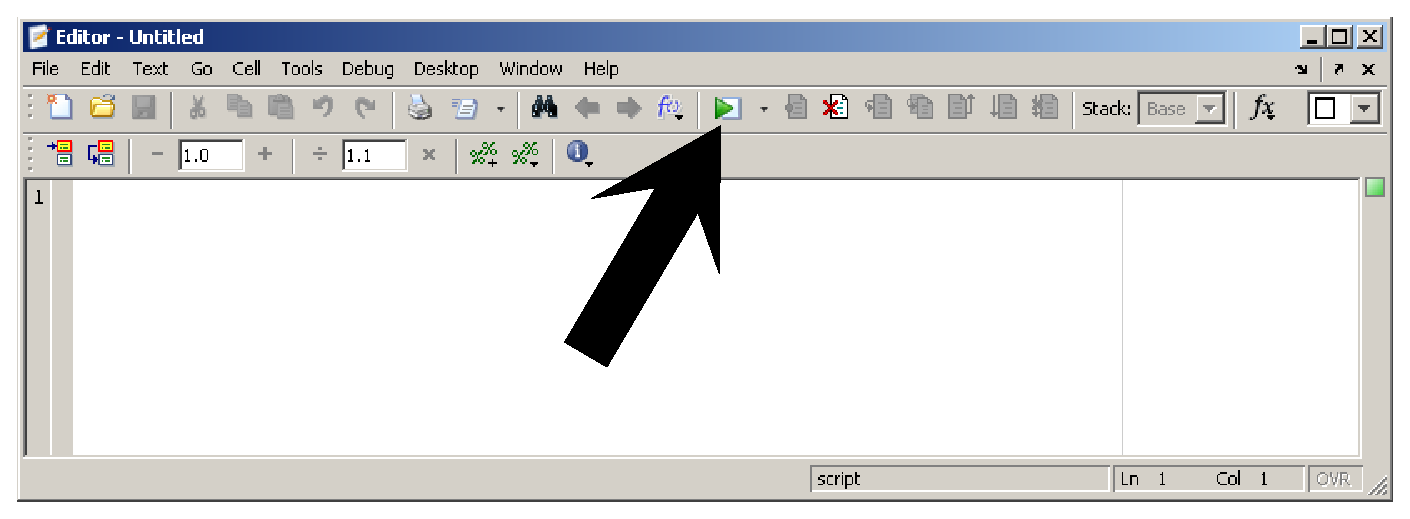
\includegraphics[width=1.0\textwidth]{./../eps/run-button.eps}}
  \caption{Location of the `run' button.}
  \label{fig:run-button}
\end{figure}


\noindent The file `demIceAge.txt' contains data on the elevation (in units of meters) of gridcells 10,000 years BP in the Gargellen valley in Austria\footnote{47.003658$^{\circ}$N,9.955546$^{\circ}$E}. 10,000 years ago, during the Ice Ages, the Gargellen Valley was under a glacier. After an increase in temperature, the ice melted and erosion created a major gully. The data file `dem2001.txt' contains the elevation (in units of meters) of the Gargellen Valley as of 2001.
\begin{action}
Load the files `demIceAge.txt' and `dem2001.txt' into the workspace. 
\end{action}




\begin{action}
Use the {\tt imagesc} command to display the contents of the variables {\tt demIceAge} and {\tt dem2001} in subplot(2,2,1) and subplot(2,2,2). Use a {\tt colorbar}\index{colorbar@\texttt{colorbar}} statement to indicate the elevation. 
\end{action}

\begin{action}
Give the subplots representative titles. 
\end{action}



\begin{action}
Calculate the difference in height between {\tt demIceAge} and {\tt dem2001} to obtain a map indicating the amount of erosion (in units of meters) over the last 10,000 years. Display this difference in subplot 3, and give it a title. 
\end{action}

\begin{action}
Given that the grid cell dimensions of both DEMs is 25 x 25 meters, calculate the total volume of rock that has been eroded in the past 10,000 years.
\end{action}

\begin{action}
Save and execute your \MATLAB{} script program.
\end{action}

\begin{action}
Before proceeding to the next project, make a review of concepts covered in Chapter \ref{ch:scripts}.
\end{action}



\hintbox{Good programming practices:
\begin{enumerate}
\item Don't forget to clear your Workspace variables when you begin to program your script files;
\item Try to limit the use of numbers in the Dynamic Part of your script (see \lstlistingname{}~\ref{list:general-structure} on page \pageref{list:general-structure}). Instead, use variables with a value that was assigned in the Initialization section;
\item Build your script by starting with the Initialization and the Output (see \lstlistingname{}~\ref{list:general-structure} on page \pageref{list:general-structure}). Then add the calculations in between;
\item Test parts of your script regularly. This is easily done by copy-pasting those parts of the script code to be tested into the \guitext{Command Window}, and then executing these parts separately. Alternatively, you can run parts of your m-file by selecting them in the editor and subsequently pressing F9 (or equivalently: right-click and choose \guitext{Evaluate Selection}).
\end{enumerate}

}%end hintbox


\project{Lead pollution in the Geul river valley}
The Geul river is located in the Province of Limburg, The Netherlands. Because of past mining activities in the area around the Geul, the river water used to contain high quantities of heavy metals including cadmium (Cd), mercury (Hg), and lead (Pb). For decades, these heavy metals have been deposited in the Geul Valley. As a result, the soil in the vicinity of the Geul river has been polluted.

The Province of Limburg wants to develop the area, but can only do so after a safety assessment has been made. Specifically, they are interested in the severity of Pb pollution in part of the valley. Cd and Hg concentrations have already been measured. These two metals do not reach dangerous concentrations and will therefore not threaten the construction plans. However, the Pb concentrations may exceed the maximum allowed concentration in parts of the valley. To investigate this, the construction companies and politicians have commissioned an assessment of the severity of the Pb pollution in the Geul valley.

More than 100 soil samples have already been taken, and a map has been constructed. Now it's up to you to manipulate and analyze this data. First, let's take a look at the Geul lead pollution data. The data are available as `geulmap.txt'. 

\begin{action}
Make sure you follow the m-file standardization guidelines for this project (see \lstlistingname~\ref{list:general-structure} on page \pageref{list:general-structure} and the Tip above). Set your work directory to `\textbackslash{}ch05\_scripts\textbackslash{}proj04\_geul' for this exercise.
\end{action}

\begin{action}
Start the m-file editor and save the empty script program as `\starred{name}\_geul.m' (with your name for \starred{name}) in your new work directory.
\end{action}

\begin{action}
Load the geulmap data into your \MATLAB{} workspace. Use {\tt imagesc} and {\tt colorbar} commands to have a quick look at the Geul river data. Let your script visualize the {\tt geulmap} data in the upper left subplot (see Figure~\ref{fig:geul}).
\end{action}




%It's important to note that the dark blue areas represent areas of zero lead concentrations. In fact no measurements were taken here. However, because these areas are much higher than the Geul river, it's assumed that there are no hazardous lead concentrations in these areas. Thus, these zero-value grid cells are not part of the Geul valley under investigation, but are included in development areas.


\begin{action}
Initially, the plan is to clean all grid cells which have concentrations in excess of 350 mg/kg. Make a 2-D logical array {\tt concMoreThan350} which is {\tt true} for indices in {\tt geulmap} that are greater than 350. Let your script visualize it in the lower right subplot. 
\end{action}

\begin{action}
Let your program calculate the total cost of having to clean all cells with concentrations in excess of 350 mg/kg, when given that the area of one grid cell is 900 m$^2$, and the cost equation for one grid cell is:
\end{action}
\begin{equation} 
TotalCost = 1000 + 1.7031 \times CellArea
\end{equation}
where $TotalCost$ is the cost in euro, and $CellArea$ is the grid cell area in m$^2$. (The correct answer is \euro~23719578).

\begin{action} 
Let your program round off the total cost to the nearest euro (see {\tt doc round}).
\end{action} 

\begin{action}
Just as you used concatenation\index{concatenation} to merge numeric arrays (see Chapter~\ref{ch:concatenation} on page~\pageref{ch:concatenation}), you can also let \MATLAB{} merge character arrays. At the prompt, create the character array {\tt string1}:
\end{action}
\prompt{string1 = \squote{My age is: }}
\noindent Now, create the \textul{character} array:
\prompt{myAge = \squote{29}}
\noindent (Note the quotes). At this point, you can merge the two strings by:
\prompt{stringBoth = [string1,myAge]}
\noindent However, you'll often find that you want to merge a character array with a numeric array, rather than two character arrays. If {\tt myAge = 29} rather than {\tt myAge = \squote{29}},
\prompt{stringBoth = [string1,myAge]}
\noindent will not yield the proper result. We can solve this by using the {\tt num2str}\index{num2str@\texttt{num2str}} function, which is used to convert numeric values to their character array respresentation.

\noindent For example, try out the following:
\prompt{clear}
\prompt{string1 = \squote{My age is: }}
\prompt{myAge = 29}
\prompt{stringBoth = [string1,num2str(myAge)]}

\begin{action}
Now let your program create a title similar to the one in the lower right subplot of Figure~\ref{fig:geul} on page~\pageref{fig:geul}.
\end{action}

\vspace{1em}
\noindent It turns out that the 350 mg/kg level was a bit too ambitious: the Province does not want to spend more than 14 million euro on cleaning the soil. It has therefore been decided that the best solution is to clean those parts where humans will be exposed to the soil (recreational areas, playgrounds and so on). After these so-called priority areas have been cleaned, the rest of the money will be used to clean as much of the valley as possible; for this part of the operation, the goal is to clean all grid cells which have a Pb concentration above a certain level.
\vspace{1em}

\begin{action}
Load the priority areas from the file `needs-cleaning.mat'. Visualize the array in the upper right subplot. Give it an appropriate title.
\end{action}

\noindent At this point, your program can visualize a logical array of concentrations above a certain level, and it can also display the logical map containing the priority areas. However, before we proceed with the project, let's digress for a moment to take a look at logical expressions (as you will see later, these are useful for the completion of the Geul project). After that, we'll come back to the Geul river project to finish up.


\section{Logical expressions}
Earlier on, we encountered relational expressions such as {\tt A$>$8}, or {\tt B$\sim=$C}. However, sometimes you want to test for more complicated relations. This is when logical expressions come in handy. Basically, there are 4 logical expressions (see also Figure~\ref{fig:logical-expressions} for a graphical explanation):
\begin{table}[ht]
\vspace{1em}
\caption{Logical expressions.}
\label{tab:logical-expressions}
\vspace{-0.5em}
\centering
\begin{tabular}{|l|c|p{8cm}|}
\hline
\textbf{Expression}&\textbf{Sign}&\textbf{Description}\\
\hline
AND&\verb#A&B#\index{\&}&The AND expression combines entries from logical arrays {\tt A} and {\tt B}, returning {\tt true} if and only if an element in {\tt A} is {\tt true} and the same element in {\tt B} is also {\tt true}.\\
\hline
OR&\verb#A|B#\index{\mid}&The OR expression combines entries from logical arrays {\tt A} and {\tt B}, returning {\tt true} if an element in {\tt A} is {\tt true} or the same element in {\tt B} is {\tt true} or when they are both {\tt true}.\\
\hline
Exclusive OR&\verb#xor(A,B)#\index{xor@\texttt{xor}}&The Exclusive OR expression combines entries from logical arrays {\tt A} and {\tt B}, returning {\tt true} if an element in {\tt A} is {\tt true} or the same element in {\tt B} is {\tt true}. It returns {\tt false} if the element is {\tt true} in both array {\tt A} and {\tt B}.\\
\hline
NOT&$\sim${\tt A}\index{$\sim$}&The NOT expression negates the values in {\tt A}, that is, what is {\tt true} will become {\tt false}, and vice versa. Is equivalent to {\tt A==0} when {\tt A} is logical.\\
\hline
\end{tabular}
\end{table}



\begin{figure}[!htb]
  \centering
    \fbox{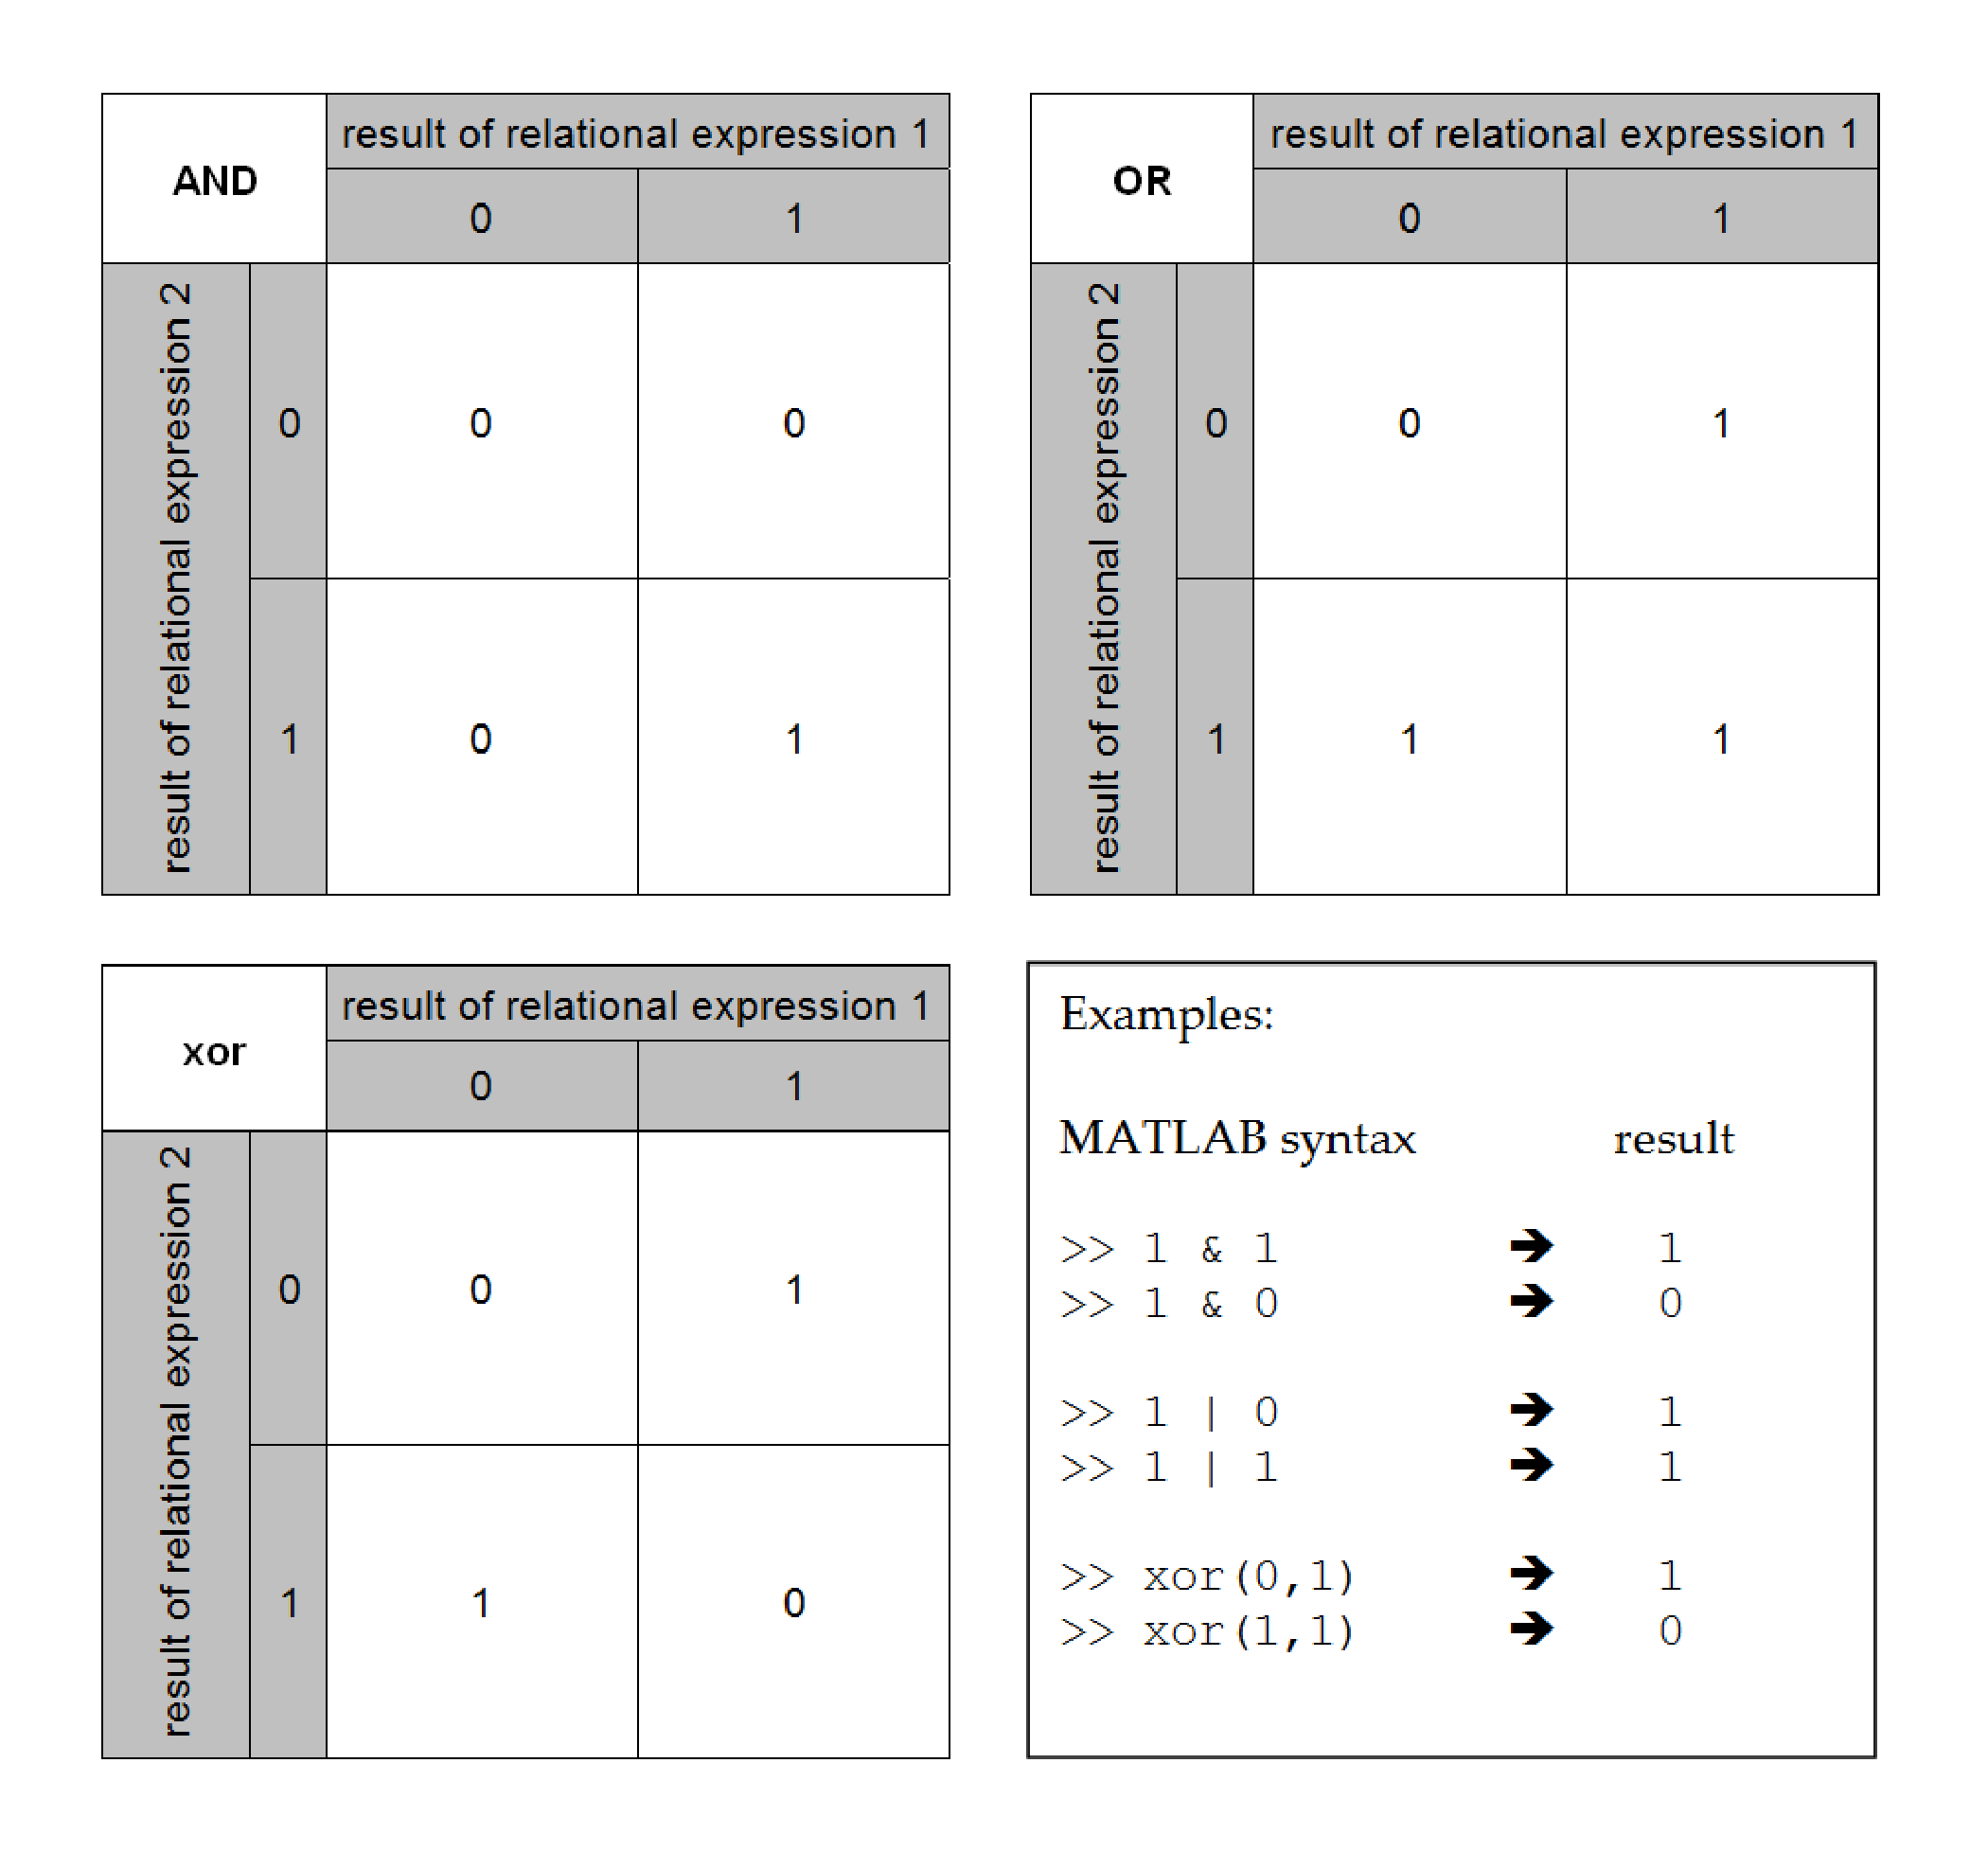
\includegraphics[width=1.0\textwidth]{./../eps/logical.eps}}
  \caption{Logical expressions.}
  \label{fig:logical-expressions}
\end{figure}


\begin{action}
Clear your workspace
\end{action}

\begin{action}
Type
\prompt{A = [2,8,0,4,3,10];}
\end{action}

\begin{action}
Type
\prompt{M = (A > 3) \& (A < 10)}
\end{action}
\begin{action}
Why would the OR-operator be useless in this example? What would be the result? 
\end{action}

\hintbox{Relational and logical operations can only be performed if the arrays are of the same size.}


\begin{action}
With this new knowledge of combining logical arrays, go back to your Geul script. What is the logical expression which allows you to create an array that has {\tt true} on all positions that need to be cleaned? (Remember that cleaning is necessary in case of high Pb concentration, or because it's a priority area).
\end{action}
\begin{action}
If you didn't already do this, change your script in such a way that you can recalculate the total cost of cleaning by changing the value of 1 variable in your program.
\end{action}
\begin{action}
Adjust the value of this variable until it meets the budget as set by the Province of Limburg, while maximizing the cleaning objective.
\end{action}


\section{Saving your variables to file}

\begin{action}
You can let \MATLAB{} save workspace variables to harddisk. For example, typing
\prompt{save(\squote{testfile.mat})}\index{save@\texttt{save}}
will save all variables that are present in the workspace to a so-called `$\ast{}$.mat-file' (extension\index{file extension} is .mat, file type is binary) which you can load at a later time.
\end{action}

\begin{action}
Execute the current exercise in the command window: Create some arbitrary variables and save them to a $\ast{}$.mat file. Now issue a {\tt clear} command. Check that your workspace is now empty. Next, load the $\ast{}$.mat file into the workspace. Check the workspace again.
\end{action}

\noindent Because it is usually unnecessary to save all the variables in your workspace to harddisk, you can also save specific variables only. If you want your files to be saved as text files instead of binary files, you must use the {\tt save} option {\tt \squote{�ascii}} to indicate the desired file format. If you choose to use the ASCII text format, your filename should have the `*.txt' extension. The {\tt save}  command can be incorporated in your script files just like any other command.

\vspace{1em}

\noindent Although the {\tt save} command can be used in a number of ways (see {\tt doc save}), its most common forms are:
\begin{lstlisting}[numbers=none]
save('safemap.txt','SafeMap','-ascii')
\end{lstlisting}
and
\begin{lstlisting}[numbers=none]
save('valley-variables.mat','SafeMap','ValleyIO','gridCellArea')
\end{lstlisting}

\noindent The first example saves the variable {\tt SafeMap} to a file `safemap.txt' containing plain text (ASCII\index{ASCII}\footnote{\url{http://en.wikipedia.org/wiki/ASCII}} essentially means `unformatted text'. You may be familiar with files that you can read with Notepad --these are ASCII files). Remember that variable names are not allowed to start with anything but a letter character (see TIP on page \pageref{tip:naming-conventions}); this way, \MATLAB{} knows that {\tt \squote{-ascii}} must be an option rather than a variable. The second example saves the 3 variables to the binary file `valley-variables.mat'. Check the \MATLAB{} help documentation for further information on the {\tt save} command.

\begin{action}
Let your program save the most important variables to a file on harddisk.
\end{action}



\begin{figure}[!htb]
  \centering
    %\fbox{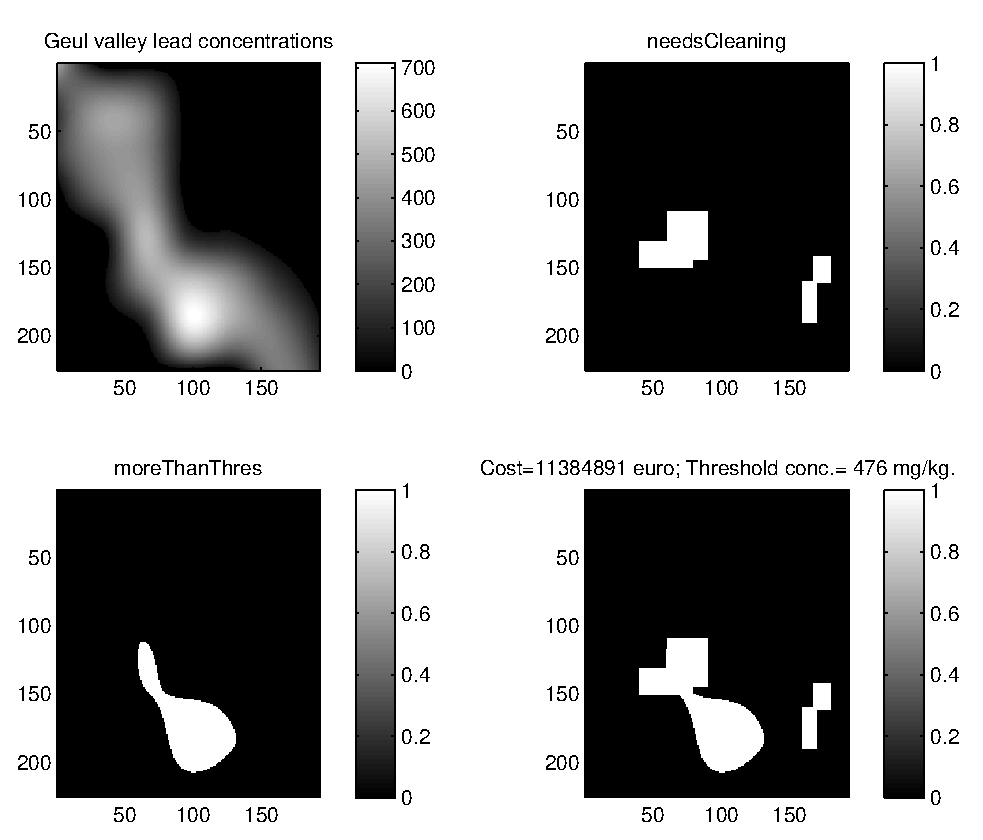
\includegraphics[width=1.0\textwidth]{./../eps/geul.eps}}
    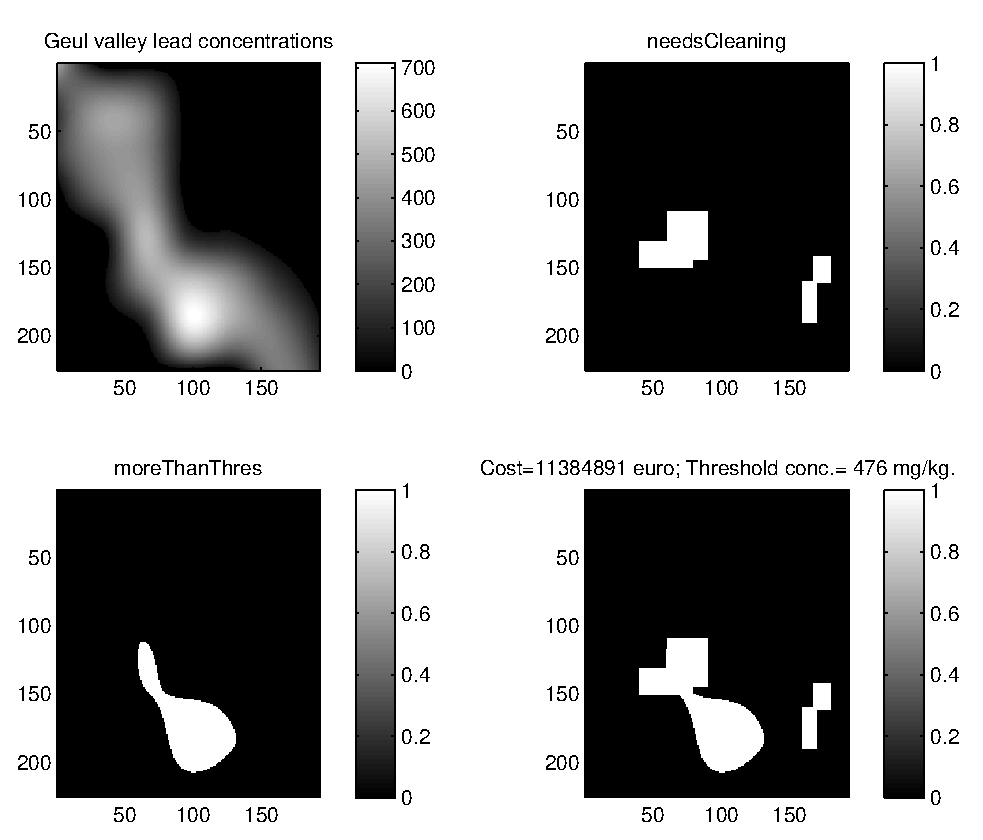
\includegraphics[width=1.0\textwidth]{./../eps/geul.eps}
  \caption{End result of the Geul pollution project. Note that the colors are different to facilitate easier interpretation when printed.}
  \label{fig:geul}
\end{figure}
\vspace{-2em}
\projectfooter

\chapter{Mathematical functions}
\thispagestyle{fancy}
\label{ch:math-functions}

\noindent Not only does \MATLAB{} provide many tools and utilities to analyze arrays, it also features a lot of mathematical commands:

\begin{table}[!ht]
\caption{Trigonometrical functions\index{trigonometrical functions}}
\label{tab:math-functions-trigonometry}
\vspace{-0.25em}
\centering
\begin{tabularx}{0.8\textwidth}{ |X|X| } \hline
\textbf{Description}&\textbf{Example}\\ \hline
sine&{\tt sin(3.1416) = -7.3464e-006}\index{sin@\texttt{sin}}\\ \hline
cosine&{\tt cos(3.1416) = -1.0000}\index{cos@\texttt{cos}}\\ \hline
tangent&{\tt tan(0.7854) = 1.0000}\index{tan@\texttt{tan}}\\ \hline
inverse sine&{\tt asin(1) = 1.5708}\index{asin@\texttt{asin}}\\ \hline
inverse cosine&{\tt acos(-1) = 3.1416}\index{acos@\texttt{acos}}\\ \hline
inverse tangent&{\tt atan(1.0000) = 0.7854}\index{atan@\texttt{atan}}\\ \hline
\end{tabularx}
\end{table}




\begin{table}[ht]
\caption{Exponential functions\index{exponential functions}}
\label{tab:math-functions-exp}
\vspace{-0.25em}
\centering
\begin{tabularx}{0.8\textwidth}{ |X|X| } \hline
\textbf{Description}&\textbf{Example}\\ \hline
exponential, $e^x$&{\tt exp(1) = 2.7183}\index{exp (base-e exponentiation)@\texttt{exp} (base-$e$ exponentiation)}\index{e!base-e exponentiation@base-$e$ exponentiation}\index{base-e exponentiation@base-$e$ exponentiation}\\ \hline
natural logarithm (base-$e$)&{\tt log(2.7183*2.7183) = 2.0000}\index{log@\texttt{log}}\\ \hline
common logarithm (base-10)&{\tt log10(100) = 2}\index{log10@\texttt{log10}}\\ \hline
square root&{\tt sqrt(25) = 5}\index{sqrt@\texttt{sqrt}}\\ \hline
\end{tabularx}
\end{table}



\begin{table}[ht]
\caption{Rounding functions\index{rounding}}
\label{tab:math-functions-rounding}
\vspace{-0.25em}
\centering
\begin{tabularx}{0.8\textwidth}{ |X|X| } \hline
\textbf{Description}&\textbf{Example}\\ \hline
round towards zero&{\tt fix(-5.7323) = -5}\index{fix@\texttt{fix}}\\ \hline
round toward $-\infty$&{\tt floor(-5.7323) = -6}\index{floor@\texttt{floor}}\\ \hline
round toward $+\infty$&{\tt ceil(-5.7323) = -5}\index{ceil@\texttt{ceil}}\\ \hline
round towards nearest integer&{\tt round(-5.7323) = -6}\index{round@\texttt{round}}\\ \hline
\end{tabularx}
\end{table}



\begin{action}
Clear your workspace by manually entering the appropriate command at the prompt and type
\prompt{G = [1:3:30];}
\end{action}


\noindent (Answer this before executing it in the command window). Consider the following command {\tt F = sin(G)}. 
\begin{action}
What are the array dimensions of {\tt F}? Check after answering.
\end{action}

\begin{action}
Clear your workspace and define a 1 x 100 array {\tt Trigo} that contains values ranging from -2*pi to +2*pi. It might be useful to take another look at the creation of \MATLAB{} utility matrices covered in chapter \ref{ch:array-ops}.
\end{action}

\begin{action}
Calculate the second row of {\tt Trigo}, containing the sine of the elements in {\tt Trigo(1,:)}.
\end{action}

\begin{action}
Create a new figure and plot {\tt Trigo}. In order to do this correctly, you must specify which vector you want to be represented on each of the axes. Assign a legend to the figure using the {\tt legend}\index{legend@\texttt{legend}} command {\tt legend(\squote{sine})}. Label the x-axis `independent variable' and the y-axis `math function'.
\end{action}

\begin{action}
Create a 1 x 60 array called {\tt Expon}, filled with equidistant values ranging from -3 to +3.
\end{action}

\begin{action}
Calculate the second row of {\tt Expon} filled with values that are exponents of the values in the first row ($10^x$ , in which $x$ is the element in the first row).
\end{action}

\begin{action}
Create a new figure and plot the second row of {\tt Expon}.
\end{action}

\begin{action}
Create a new figure and use the {\tt semilogy}\index{semilogy@\texttt{semilogy}} command to display the second row of {\tt Expon} in a plot with a logarithmic y-axis. Consult the help documentation for information on the use of {\tt semilogy}.
\end{action}

\begin{action}
Type {\tt ylabel(\squote{10\^{}{x}})} and confirm that it is displayed as $10^x$, then set the color of the sine in figure 1 to {\tt {\squote{r}} (red).
\end{action}


\noindent \lstlistingname{}~\ref{list:plot-example} contains an example of how to use the {\tt plot} function. (Note that it is slightly different from what you just did).
\lstinputlisting[float=ht,caption={Example of how to use the {\tt plot} function},label=list:plot-example]{./../pim_files/ch06_math/plot_example.m}

\chapter{Function m-files}
\thispagestyle{fancy}
\index{function m-files}
\label{ch:functions}


\MATLAB{} functions such as {\tt sin}, {\tt sqrt}, {\tt linspace} and {\tt find} take the variables you enter and perform the operations specified in these functions. The commands executed inside the function, as well as any intermediate variables created by these commands, are hidden. These variables exist in a part of the workspace that is separate from the top level (or `Base' workspace\index{base workspace}) that you have worked with so far. The lower level of the workspace is sometimes referred to as `function workspace'\index{function workspace}. In a way, function m-files are like a black box: all you see is the input that goes in and the output produced by the function. Functions provide a very powerful way to modularize your program. Modularity\index{modularity} is useful, because it lets you structure your computer program. Because variables that are created by a function `live' in a separate part of the workspace, they cannot interfere with variables outside the function workspace. This means that you can have a variable {\tt X} defined in the base workspace, as well as in the function workspace. Changing the value of {\tt X} in the function will not affect the value of {\tt X} in the base workspace, unless you explicitly tell \MATLAB{} that you want this by including {\tt X} as a output variable. 

Function m-files are similar to \MATLAB{} script m-files\index{script m-files} in that they are text files with a~*.m extension. Also, like script m-files, function m-files are not entered in the command window but rather are external text files created with a text editor. However, a function m-file is different from a script m-file in that it begins with the `function definition line'\index{function definition line}, which has to be the first command line in the m-file, and has to start with the word ``function''\index{function@\texttt{function}}. This way, \MATLAB{} knows that the commands inside the m-file need to be executed in a separate workspace. 

\vspace{1em}
\noindent The function definition line always has the following structure (in order of appearance):
\begin{enumerate}
\item{the word {\tt function};}
\item{zero, one, or more output variables. If there is more than one output variable, they need to be enclosed in square brackets `{\tt [ ]}'. Multiple variables need to be separated by commas;}
\item{the is-equal sign `=';}
\item{the name of the function. Its use here is only for completeness: When \MATLAB{} encounters a function name in a script m-file, it starts looking for an m-file by that name as it is known by the operating system (Windows, Linux etc). For instance, when you call the function {\tt mean}, \MATLAB{} uses the code from a file called `mean.m' residing somewhere on your harddisk. Because some operating systems are case-sensitive with respect to filenames, you may only use lowercase characters in your script and function filenames.}
\item{the last part of the function definition line lists the input variables. This part may contain zero, one, or more input variables. The variables need to be enclosed in parentheses `{\tt ( )}'. Multiple variables need to be separated by commas.}
\end{enumerate}
\lstlistingname{}~\ref{list:function-definitions} gives a few examples of valid and invalid function definition lines.
\lstinputlisting[float=ht,caption={Various function definitions for a file called `calcflow.m'},label=list:function-definitions]{./../m/function_definitions.m}



\hintbox{Variables that are passed to a function, or that are returned by a function, are referred to as `input arguments'\index{input arguments}\index{arguments!input arguments} and `output arguments'\index{output arguments}\index{arguments!output arguments}, respectively.}


\section{Writing function m-files}

\begin{action}
Study the function m-file `statsm.m' located in the folder `\textbackslash{}ch07\_functions' (see \lstlistingname{}~\ref{list:statsm}).
\end{action}
\lstinputlisting[float=p,caption={Contents of the file `\textbackslash{}ch07\_functions\textbackslash{}statsm.m'},label=list:statsm]{./../m/statsm.m}
As can be seen in this example, the function definition line of a function m-file defines the m-file as a function, specifies its function name ({\tt statsm}), and defines its input ({\tt M}) and output ({\tt MaxM}, {\tt MinM}, {\tt MeanM}) variables. Following the function definition line is a sequence of comment lines, as indicated by the percent sign. The comment lines are meant to provide information about the function m-file. 


\begin{action}
Make sure you are in the right directory and type:
\prompt{help statsm}
\end{action}
As you can see, \MATLAB{} returns the first block of comment lines upon typing {\tt help}. This is useful when you forgot how a particular function works; however, it does mean that you have to provide the help comment block in the m-files that you produce. Note: any blank lines before the {\tt \%} sign in this first comment line disqualifies it from being displayed. 

Ideally, the first comment block should start with some keywords (line 2 in \lstlistingname{}~\ref{list:statsm}), followed by a line that states how the function must be called (line 3). The help comment should also contain a description of what it does (line 4), its input and output variables, including the array type, array dimensions, and a short description (lines 5--8). Additionally, it should contain information on the author of the file (line 10), the date (line 10), and the \MATLAB{} version that was used to develop the software (line 11).



\section{Using a function in your script}

In contrast to script m-files, a function m-file cannot run by itself. Instead, function m-files are usually called by a script m-file. The function's input variables must be present in the workspace before evaluating the function call\index{function call}. The input arguments can then be passed on to the function, where they get processed by the code in the function m-file. \lstlistingname~\ref{list:stats_lux} provides an example of how the function {\tt statsm} (see \lstlistingname~\ref{list:statsm}) may be used.

\lstinputlisting[float=p,caption={Contents of the file `\textbackslash{}ch07\_functions\textbackslash{}stats\_lux.m'},label={list:stats_lux}]{./../m/stats_lux.m}



\subsection{Workspaces and code re-use}
\begin{action}
Open `stats\_lux.m' in the editor and run it. After the program finishes, why isn't there a variable {\tt M} in the workspace?
\end{action}
Note that the arrays {\tt MaxLux}, {\tt MinLux}, {\tt MeanLux} and {\tt dem\_lux} in {\tt stats\_lux} contain the same information as {\tt MaxM}, {\tt MinM}, {\tt MeanM} and {\tt M} in {\tt statsm}. This is yet another useful feature of functions: because your function has its own workspace, it does not have to use the same variable names as your script. What's very important though, is that you have to pass your arguments in the right order for this to work correctly. The system of order-based argument passing allows you to re-use your code\index{code re-use}, without having to adapt the code inside the function. 
\begin{action}
Take 5 minutes to think about what you would have to change in {\tt statsm} if the arguments would always be called the same inside the function workspace, as compared to outside).
\end{action}


%When the main program is run from \MATLAB{}, it calls the function m-file {\tt statsm} that is embedded in its program (line 15) and then enters this function with the input variable dem\_lux . Directly after entering statsm, the information from dem_lux has entered the function's workspace and is now (locally) known as M. You can see this for yourself in the source code of 'statsm.m'. When all calculations in statsm are executed, the output (locally known as MaxM, MinM and MeanM ) is returned to the main program. Directly after leaving the function, the information from MaxM, MinM and MeanM is present in the workspace as MaxL, MinL and MeanL respectively.
%
%



\begin{action}
Create your own function m-file that extends {\tt statsm} by also calculating the standard deviation of all values in the matrix {\tt M}. Save the altered m-file as `\starred{name}\_statsm.m'. Adapt the script in accordance with your function. Save it as `\starred{name}\_stats\_lux.m'. (The correct answer for the standard deviation of the height in the study area Luxemburg is 64 m).
\end{action}



\noindent 
\begin{minipage}[]{\textwidth}{\vspace{2em} \hrule \vspace{1em} \centering \begin{minipage}[]{0.8\textwidth}{\textsc{\textbf{Summary of why functions are useful\,}} \small 

\vspace{0.5em}


\noindent Many script m-files contain function m-files for certain calculations. Why use function m-files if you can simply enter the calculation command lines in the script m-file itself?

\vspace{1em}
\noindent Functions have some major advantages:
\begin{enumerate}
\item{In many cases, script m-files in which all calculations are entered in one file can become too long to read and difficult to understand. Those script m-files with thousands of command lines are far from user-friendly. The use of function m-files offers the possibility to organize the program, making it easier to understand.}
\item{A function m-file can be called an infinite number of times within a program. Instead of writing command lines for similar calculations over and over in an m-file, one function m-file can perform these calculations every time with new input arguments and have the result returned to the main program through its output arguments.}
\item{Variable names in the function m-file are local and will not appear in your workspace: they exist only within the function. You have almost complete freedom in naming input and output arguments in the function itself, just follow the guidelines in the TIP on page \pageref{tip:naming-conventions}. As indicated previously, use logical and easy-to-understand names for your input and output variable names.}
\end{enumerate}


}\end{minipage} \vspace{0.5em}
\hrule \vspace{2em} \end{minipage}}





\subsection{Multiple calls}

The function definition line dictates the manner in which function m-files have to be incorporated into the main program. Suppose we have a main program in which a function m-file is used to convert degrees to radians (\lstlistingname{}~\ref{list:slope_dir_script}).

\lstinputlisting[float=ht, caption={Contents of the file `\textbackslash{}ch07\_functions\textbackslash{}slope\_dir\_script.m'},label=list:slope_dir_script]{./../m/slope_dir_script.m}
\lstinputlisting[float=ht, caption={Contents of the file `\textbackslash{}ch07\_functions\textbackslash{}conv\_deg2rad.m'},label=list:conv_deg2rad]{./../m/conv_deg2rad.m}\label{lab:conv_deg2rad}


\noindent The main program {\tt slope\_dir\_script} defines the input variables to be processed by the function m-file {\tt conv\_deg2rad} (See \lstlistingname{}~\ref{list:conv_deg2rad}). Note that {\tt conv\_deg2rad} will convert any number to radians as long as the syntax is correct (that is, you didn't make a `spelling' or `grammar' mistake)\index{syntax}. For example, {\tt conv\_deg2rad} is used first to convert a direction, after which it is used a second time to convert a slope angle. Even though the meaning of {\tt DirDeg} is different from that of {\tt SlopeDeg}, it is not necessary to change the contents of `conv\_deg2rad.m'.


\begin{action}
Is it useful to include the {\tt clear} command in a function m-file? Why (not)?
\end{action}

\noindent So far, we have encountered functions that were called by scripts. However, functions can also be called by other functions. We will see an example of this during project \ref{pr:reisdorf}.
\chapter{Control flow}
\thispagestyle{fancy}

A boulder lying on a slope will slide downslope if the friction between the boulder and the hillslope decreases below a certain threshold value. Mass wasting of this type can occur when surface friction is lowered by rainfall:
 
\lstinputlisting[caption={},nolol,numbers=none]{./../m/rockfall.m}

\noindent This is an example of how you can let \MATLAB{} decide which parts of a program should be evaluated: depending on the outcome of the test {\tt friction < threshold}, either the {\tt if...else} bit or the {\tt else...end} bit is evaluated. Besides the dynamic decision-making capability of the {\tt if}-{\tt else}-{\tt end} structure, \MATLAB{} provides code structures which allow for the repeated execution of a set of commands (a so-called `loop'\index{loop}). Termination of the loop can be because it is set to run a predetermined number of times, or because a certain condition is satisfied. The former is known as a {\tt for}-loop\index{for-loop@\texttt{for}-loop}, while the latter is known as a {\tt while}-loop}\index{while-loop@\texttt{while}-loop}. {\tt if}-{\tt else}-{\tt end} structures, {\tt for}-loops and {\tt while}-loops are examples of `control flow' structures\index{control flow}. Because these constructions often encompass multiple \MATLAB{} commands, they are mostly used in scripts and functions (as opposed to at the prompt).


\section{for-loops}
\label{sec:for-loops}
\index{loop!for}
\index{for@\texttt{for}}
\index{end@\texttt{end}}
{\tt for}-loops allow a group of commands to be repeated a fixed, predetermined number of times. The general form of a for-loop is:
\lstinputlisting[nolol,numbers=none]{./../m/general_for_loop_structure.m}\label{ind:rowvector}
\begin{action}
Execute the following (in a new script):
\lstinputlisting[nolol,numbers=none]{./../m/simple_for_loop.m}
\end{action}
\noindent Be aware that the above is equal to the so-called `vectorized'\index{vectorization}\label{ind:vectorization} way of programming: 
\lstinputlisting[nolol,numbers=none]{./../m/simple_for_loop_vectorized.m}
\noindent It is up to you to decide which form is better suited for specific cases. Be aware that \MATLAB{} performs its calculations faster if you use vectorization. Loops, however, are usually easier to understand. Also, some problems can not be adequately handled by vectorized programming. 

\subsection{Malthusian population growth}

One of the first researchers into population dynamics was Thomas Malthus\footnote{\url{http://en.wikipedia.org/wiki/Thomas_Malthus}}, (1766--1834). In his `Essay on the Principle of Population' (1798) Malthus observed that in nature plants and animals produce far more offspring than can survive, and that Man too is capable of overproducing if left unchecked. This exponential growth is known as Malthusian population growth; the rate at which a population grows is directly proportional to its size.

Pierre-Fran\c cois Verhulst\footnote{\url{http://en.wikipedia.org/wiki/Pierre_Fran\%C3\%A7ois_Verhulst}} (1804--1849) was a Belgian mathematician who generalized the Malthusian model by allowing for the fact that populations encounter internal competition as they grow within a closed environment, and this competition has a tendency to retard the rate of growth. His idea says that while the population will continue to grow as time goes on, the rate at which it does this growing gets smaller. This is a slightly more realistic approach than that of Malthus, whose idea actually predicts that populations will grow exponentially, and without bound --a prospect that defies physical limitations. 

The script m-file `\textbackslash{}pim\_files\textbackslash{}ch08\_control\_flow\textbackslash{}malthus.m' contains part of the program that calculates population size over time based on the ideas of Malthus and Verhulst. The exponential growth and competitive growth decline are expressed in Equations~\ref{eq:verhulst-term}--\ref{eq:malthus-verhulst}:


\begin{equation}
\label{eq:verhulst-term}
V=1-\frac{P_{now}}{P_{max}}
\end{equation}
\begin{equation}
\label{eq:malthus-verhulst}
P_{next}=P_{now}+r*P_{now}*V
\end{equation}
where $V$ is the Verhulst term, $P_{max}$ is the maximum sustainable population size, $P_{now}$ is the current population size, $P_{next}$ is the population size for the next time step, and $r$ is the growth factor.

\begin{action}
Complete the Verhulst term in `malthus.m'.
\end{action}
\begin{action}
Study `malthus.m' and identify which role each variable has. Next, implement Equation \ref{eq:malthus-verhulst} in the for-loop.
\end{action}
\begin{action}
In Section \ref{sec:for-loops}, we saw that some problems can be vectorized. Is this such a problem? Why (not)?
\end{action}


\section{while-loops}
\label{sec:while-loops}
\index{loop!while}
\index{while@\texttt{while}}
\index{end@\texttt{end}}

As opposed to a {\tt for}-loop that evaluates a group of commands a fixed number of times, a {\tt while}-loop evaluates a group of statements as long as a certain condition is true. The general form of a {\tt while}-loop is:
\lstinputlisting[nolol,numbers=none]{./../m/general_while_loop_structure.m}

\noindent The assignment statements between the {\tt while} and {\tt end} statements are executed as long as the {\tt expression} is true. This implies that the {\tt while}-loop can only be terminated if one of the variables in {\tt expression} is changed \textit{inside} the {\tt while}-loop.

\begin{action}
Study the example script m-file in \lstlistingname~\ref{list:example-while}:
\end{action}
\lstinputlisting[caption={Example of a {\tt while}-loop}, label=list:example-while,numbers=none]{./../m/example_while.m}

\noindent Note that the variable {\tt Steps} needs to be converted from numerical value (double array) to text (char array) by the {\tt num2str(Steps)}\index{num2str@\texttt{num2str}} command to allow for concatenation with the character array {\tt \squote{Maximum value reached. Steps = }}. After that, the resulting character array can be output to the command window by the function {\tt disp}\index{disp@\texttt{disp}} (see \MATLAB{} documentation). 

\hintbox{By clicking in the command window and simultaneously pressing Ctrl-c, you can stop calculation anytime.}


\begin{action}
Write a script m-file with a {\tt while}-loop that never terminates.
\end{action}

\begin{action}
How would you characterize the difference between a {\tt for}-loop and a {\tt while}-loop? When would you use one or the other? Give an example of each.
\end{action}



\hintbox{One of the most common mistakes concerning control flow is the never ending {\tt while}-loop. A helpful rule of thumb is that the variables which are in the {\tt expression} have to be changed inside the {\tt while}-loop, otherwise it can never terminate.}


\section{if-else-end}
\index{if@\texttt{if}}
\index{else@\texttt{else}}
\index{end@\texttt{end}}


Many times, sequences of commands must be conditionally evaluated based on a relational test. Recall our first control flow example:
\lstinputlisting[caption={},nolol,numbers=none]{./../m/rockfall.m}

\noindent Based on the outcome of the relational test {\tt friction < threshold}, either the command sequence between the {\tt if} and {\tt else} statements is called, or the command sequence between the {\tt else} and {\tt end} statements is called.

\vspace{1em}

\noindent When there are three or more alternatives, the {\tt if-}{\tt else}-{\tt end} construction takes the form: 
\lstinputlisting[caption={},nolol,numbers=none]{./../m/general_elseif.m}\index{elseif@\texttt{elseif}}

\noindent In this construction, only the commands associated with the first true expression encountered are evaluated; all following relational expressions are not tested, and the rest of the {\tt if-}{\tt else}-{\tt end} construction is skipped. Furthermore, the final {\tt else} command may or may not appear.

\vspace{1em}
\noindent An application of {\tt if-}{\tt else}-{\tt end} will appear in the next chapter.
 


\chapter{Using the debugger}
\thispagestyle{fancy}
\label{ch:debugging}

In the process of programming m-files, it is inevitable that errors, also known as bugs\index{bug}, will occur. \MATLAB{} provides some functionality to assist in \textit{debugging}\index{debugging} m-files. Two types of errors can occur in \MATLAB{} expressions: syntax errors\index{syntax error} and run-time errors\index{run-time error}. 

\section{Syntax errors}
Syntax errors (such as misspelled variable names, misspelled function names, missing quotes or parentheses, incorrect use of special characters, etc.) are found when \MATLAB{} is preparing to run the program. \MATLAB{} flags these errors immediately upon execution of the program and provides feedback about the type of error encountered and an estimate of the line number in the m-file where it occurs. Given this feedback and some experience, these errors are usually easy to spot.

\section{Run-time errors}
Run-time errors (programming errors such as zero divided by zero) are generally more difficult to find, because you can't tell just from looking at the code that it will generate an error. For example, your script may contain an addition {\tt A = B + C}, which you would not expect to contain an error. However, if the arrays {\tt B} and {\tt C} do not have the same size, \MATLAB{} will raise an error.

\section{Manual debugging}
In script m-files, you can monitor all calculation steps and variables by executing the command lines of the script m-file one by one in the command window. In this way, errors can usually be spotted quickly. In function m-files however, variables only exist as local variables living in their own part of the workspace away from the base workspace. This can make monitoring of the calculations and variables within functions very difficult.

There are several approaches to debugging function m-files. For simple problems, the easiest way to find bugs is to use a combination of the following:

\begin{enumerate}
\item {Remove semicolons within the function so that intermediate results are displayed in the command window;}
\item {Add statements that display variables of interest within the function;}
\item {Change the function m-file into a script m-file by placing a \% before the function definition statement at the beginning of the function m-file. When executing as a script file, the workspace is the \MATLAB{} workspace, and thus it can be interrogated after the error occurs. Declare input variables in the Command Window, otherwise they won't be present in the workspace;}
\item {Inserting a {\tt pause}\index{pause@\texttt{pause}} or {\tt keyboard}\index{keyboard@\texttt{keyboard}} command (e.g. in loops) enables you to view changes in your variables step by step (Refer to the documentation for the use of these functions).}
\end{enumerate}

\noindent When an m-file consists of multiple functions, or functions are called within functions, these methods are often not enough to efficiently debug your programs. For such problems, you must use the \MATLAB{} Debugger.


\section{Debugging in the Editor}
\begin{action}
Use the editor to open `000\_debugscript.m' and `000\_pfilt.m' (located in the folder `\textbackslash{}ch09\_debugging'). Click on \guitext{File} in the editor's menu and select \guitext{Save as\ldots}.
\end{action}


\begin{action}
Substitute your own last name for the zeros in the filenames.
\end{action} 

\begin{action}
Adapt the function call of {\tt 000\_pfilt} in {\tt 000\_debugscript} in accordance with the new name of the function m-file.
\end{action}


\noindent {\tt debugscript} is a simple program that uses the function {\tt pfilt} to filter a data set based on the deviation from the mean. However, the program is not functioning properly. Unfortunately, it is always very difficult to trace the bugs in someone else's program. You will need the \MATLAB{} debugger to help you.


\begin{action}	
Check for errors in the script {\tt debugscript} by running it from within the m-file editor.
\end{action}

\begin{action}
To be able to use the Debugger effectively, you need to arrange the GUI in such a way that you can see the editor window as well as the command window and the workspace. An easy way to do so is by clicking the \guitext{Dock Editor}-menu item under \guitext{Desktop} in the m-file editor's menu (see Figure \ref{fig:dock-editor}).
\end{action}


\begin{figure}[!htb]
  \centering
    \fbox{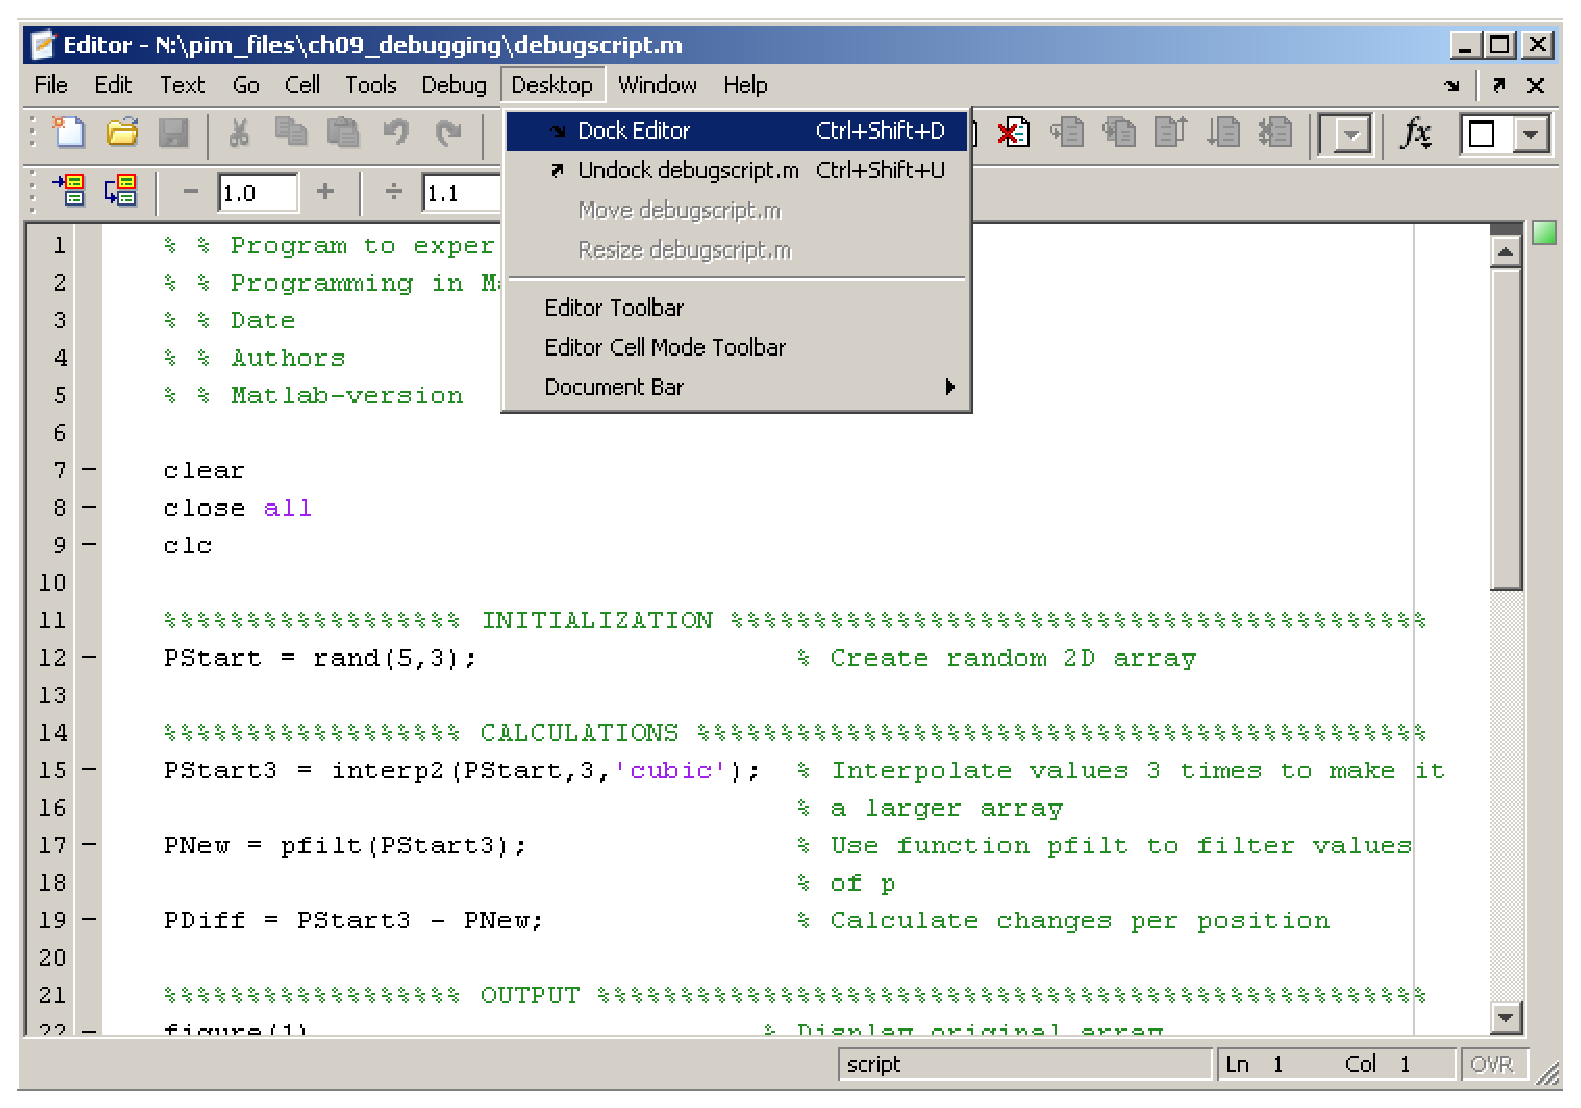
\includegraphics[width=1.0\textwidth]{./../eps/dock-editor.eps}}
  \caption{Docking the m-file editor.}\label{fig:dock-editor}
\end{figure}






\noindent Two errors occur somewhere in {\tt pfilt}. Because the variables in {\tt pfilt} live in the function workspace, monitoring of these variables is not straightforward. You can use the debug options in the Editor to trace and fix these errors. 

Note: to be able to use the debugging functionality, make sure that you have started the m-file editor from the command window using the {\tt edit} command. Also, if the editor window has been docked into the \MATLAB{} window, make sure that it is the active window by clicking anywhere in your m-file.

In order to use the debugger, you have to set breakpoints first. These breakpoints define where calculations will be (temporarily) stopped in the debug mode. You can set a breakpoint by clicking on one of the dash signs in the m-file editor's margin. Alternatively, you can move your cursor to a line and press the F12 button to set a breakpoint on that line. If you want, you can set multiple breakpoints. After a breakpoint has been set, a marker appears in the margin on that line (see Figure \ref{fig:set-breakpoint}). The color of this marker can be red or gray. If it is red, that means that the script in which your breakpoint has been set, was not changed since you saved it. If it is gray, that means that you have changed your m-file since the last time you saved it. 

\hintbox{Before running your file, you should always make sure that you saved it.}


\begin{figure}[!ht]
  \centering
    \fbox{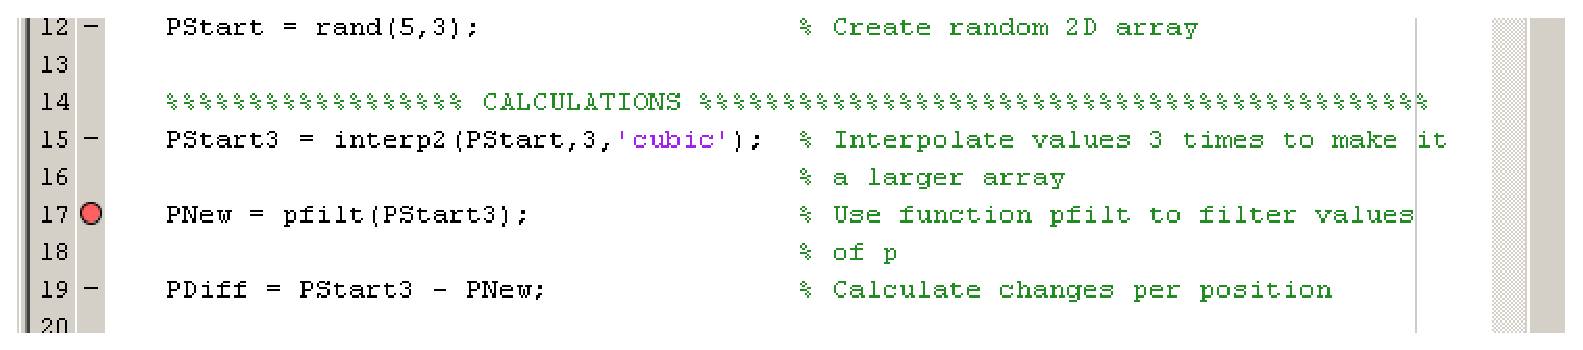
\includegraphics[width=1.0\textwidth]{./../eps/set-breakpoint.eps}}
  \caption{A breakpoint has been set.}\label{fig:set-breakpoint}
\end{figure}


\noindent By pressing F5 or clicking the \guitext{Run} button, the commands in the active m-file will be evaluated line by line until the end of your m-file is reached, or until the first breakpoint, whichever comes first. Breakpoints are usually set a few lines up from where you suspect an error. If you don't have any idea as to where an error occurs, you can set your breakpoint on the first line of the file. If you press F5 when any breakpoints exist in your m-file or in one of the functions it uses, \MATLAB{} will go to the debug mode. In the command window, the {\tt $>>$} is changed to {\tt K$>>$} to indicate the debug mode ({\tt K} for `keyboard'). If the commands in your m-file can be evaluated successfully up to the point where the breakpoint has been set, a green arrow appears on the breakpoint's line (see Figure \ref{fig:run-to-breakpoint}). After the breakpoint is reached, control is returned to the user and variables can be checked and commands entered at the prompt.

\begin{figure}[!ht]
  \centering
    \fbox{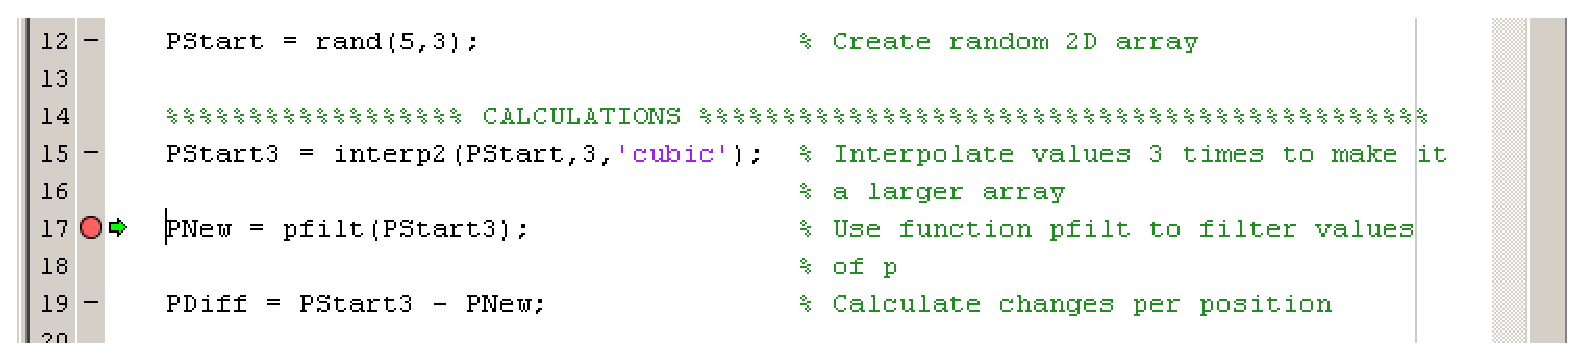
\includegraphics[width=1.0\textwidth]{./../eps/run-to-breakpoint.eps}}
  \caption{{\tt debugscript} has been evaluated successfully up to the breakpoint.}\label{fig:run-to-breakpoint}
\end{figure}

\vspace{1em}
\noindent Up to this point, debugging has been very similar to simply entering your commands one by one at the prompt. However, as soon as one of those commands happens to be a function (in which an error occurs), you will not be able to monitor the variables in the function's workspace by simply entering them at the prompt, since a function is somewhat like a black box: only the function's output arguments are returned to the base workspace. Because you cannot see the changes in the function's variables, finding the error in your function can become very difficult. The debugger, however, offers some useful tools to assess where the error is coming from.

If a breakpoint has been set and the commands can be evaluated successfully up to the breakpoint (in other words: if you have a green arrow), you can use \guitext{Step} from the \guitext{Debug} menu to go through your m-files line by line. Alternatively, you can press the F10 button. 

\begin{action}
Set a breakpoint at the very first command line (i.e. next to {\tt clear}) and run through your file line-by-line with the step function. Monitor how new variables are added to your workspace while you step through it.
\end{action}
\hintbox{You might have to right-click your workspace window and select \guitext{Refresh} to see the changes to your variables.}
\noindent If you try to step past the function call line at line 17, you will notice that \MATLAB{} returns an error. Apparently, the error is generated by some command used in the {\tt pfilt} function. Besides stepping through your m-file line-by-line by pressing F10, you can also step into functions with the input arguments that were calculated in the script.

\begin{action}
Set a breakpoint at the function call line of {\tt pfilt} and run your script m-file up to that point. List the variables that are present in your workspace.
\end{action}

\begin{action}
Now, select \guitext{Step in} from the \guitext{Debug} menu (or, equivalently, press F11) to step into the {\tt pfilt} function with the input argument(s) necessary for the successful execution of {\tt pfilt}.
\end{action}

\begin{action}
The green arrow should now be right next to the first command line in {\tt pfilt}. Compare your workspace with the list of variables you made a moment ago. Where did all the variables go? And where did {\tt In01} come from? What information does it contain?
\end{action}



\noindent The great advantage of using \guitext{Step in} is that the workspace will contain the locally declared variables, which enables the explicit, step-by-step monitoring of your variables, even within function m-files.

 
\hintbox{Pressing `F5' or clicking the \guitext{Run} button when the active m-file is a function, will return an error:\newline\newline
{\tt ??? Input argument \squote{In01} is undefined.\newline\newline}
This is because trying to run a function on its own will cause the function's input arguments (in this case {\tt In01}) to remain undefined.
}
\noindent If you step into a function, the green arrow in the parent m-file (in this case {\tt debugscript}) changes into a white arrow (see Figure \ref{fig:breakpoint-white-arrow}). This indicates that {\tt debugscript} is not the file that you are currently in. Therefore, any variables displayed in the workspace window do not belong to this (parent) m-file. 


\begin{figure}[!ht]
  \centering
    \fbox{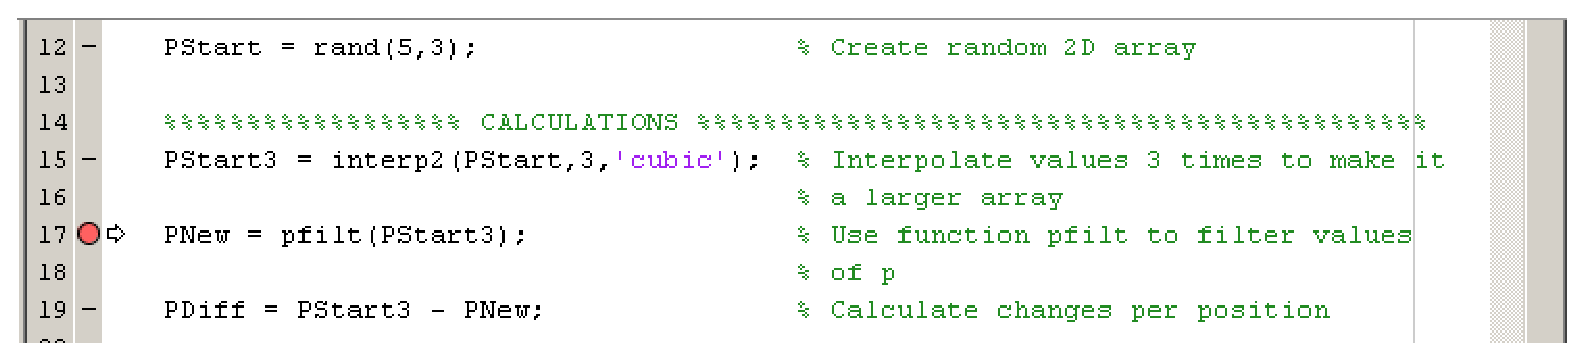
\includegraphics[width=1.0\textwidth]{./../eps/breakpoint-white-arrow.eps}}
  \caption{A white arrow in the parent m-file shows that it is not the active file.}\label{fig:breakpoint-white-arrow}
\end{figure}


\begin{action}
Use the \guitext{Step} function in {\tt pfilt} and check your workspace. Let the debugger execute command lines in {\tt pfilt} one at a time and continue to monitor the variables in your workspace. Monitoring of the variables in the workspace involves:
\begin{enumerate}
\item variable values;
\item variable names (pay attention to lowercase/uppercase)
\item variable dimensions (check the workspace column 'size') or type {\tt >> whos}
\item variable class (what is the data type of the variable under consideration?) For an overview of data classes, check Chapter \ref{ch:arrays}.
\end{enumerate}
\end{action}

\begin{action}
What problem arises when {\tt MinCrit} and {\tt MaxCrit} are calculated? What is the reason for this problem? Alter the command lines to solve this problem.
\end{action}

\noindent You have now corrected one of the errors in {\tt pfilt}. However, when running {\tt debugscript}, \MATLAB{} still returns an error message. Considering the output arguments of the function {\tt pfilt}, what command would you expect to be on the last line of this m-file?

\begin{action}
Correct the last error in {\tt pfilt}. Use the debug tools if necessary.
\end{action}


\noindent \guitext{Exit Debug Mode} from the \guitext{Debug}-menu will exit the debug session and invoke the normal mode indicated by the $>>$ sign. The debug mode can be exited at any time during debugging.

\hintbox{The \guitext{Stop if errors/warnings\ldots} in the \guitext{Debug} menu allows you to stop calculations right before an error or warning occurs. This functionality can be especially helpful when debugging loops.}


\noindent Before proceeding with the next chapter, make a review of the concepts covered in Chapters \ref{ch:math-functions}--\ref{ch:debugging}.



\chapter{Infinity and missing values}
\thispagestyle{fancy}
\label{ch:infinity-etc}



Since a computer is a discrete and finite machine, certain operations are undefined:
\begin{action}
Type 
\prompt{10/0}
\end{action}
The result of this operation is {\tt Inf}\index{Inf@\texttt{Inf}}. {\tt Inf} is the arithmetic representation for positive infinity ({\tt -Inf} for negative infinity). Infinity results from operations like division by zero and overflow (calculations that lead to results too large to represent as conventional floating-point values).
\begin{action}
Type 
\prompt{0.0/0.0}
\end{action}
The result of this (illegal) operation is {\tt NaN}\index{NaN@\texttt{NaN}}: Not-a-Number. A {\tt NaN} result is obtained because of mathematically undefined operations. Undefined operations that produce {\tt NaN}: 
\begin{enumerate}
\item any arithmetic operation on an array containing {\tt NaN}
\item division, such as {\tt 0/0} and {\tt Inf/Inf}
\end{enumerate}
Often {\tt NaN}s occur in imported data.
\begin{action}
Type
\prompt{A = [1,2,3;4,NaN,6;7,8,9]}
\end{action}
\begin{action}
Try to calculate the mean and standard deviation of {\tt A}.
\end{action}
Because arithmetic operations on {\tt Inf} or {\tt NaN} produce {\tt Inf} or {\tt NaN}, it is necessary to remove or replace these values in arrays before further calculations.
\begin{action}
Type
\prompt{B = [123,Inf,43.2,18,28,NaN,pi,exp(1),-Inf,4]}\index{pi@\texttt{pi}}
\end{action}
\begin{action}
Type
\prompt{Bnan = isnan(B)}\index{isnan@\texttt{isnan}}
and
\prompt{Binf = isinf(B)}\index{isinf@\texttt{isinf}}
and interpret the results. Take a look at the data classes of the variables listed in the workspace.
\end{action}
\begin{action}
Use {\tt isnan}, {\tt isinf} and {\tt find} in combination with logical and relational operators to create an array {\tt BFinite} that contains only those values of {\tt B} that are not {\tt NaN} or {\tt Inf}. Use only one command line. The result {\tt BFinite} should be an 1x7 array.
\end{action}

\project{Aluminum toxicity}
\label{pr:aluminum-toxicity}
Often, the data you import or create during programming contain errors. Values such as {\tt NaN}, {\tt -Inf}, and {\tt Inf} can occur in a data set as a result of measurement errors or illegal mathematical operations. Because statistical operations are impossible on these values, it is sometimes necessary to remove them from your data before further calculation.

Aluminum (Al) is a common element found in sandy soils. At pHs up to about 4.5, Al$^{3+}$ is the most common form of Al. At higher pHs, the Al can form complexes and become immobile in the soil environment. The `free' Al$^{3+}$-ion is mobile and can be transported easily with the soil water. This way plants can take up Aluminum, which is an important nutrient. However, high Al$^{3+}$ concentrations can become toxic to plants, inhibiting growth or even causing death. Evaluating concentrations of Al$^{3+}$ is important in determining the toxicity hazards in ecosystems. In the Dutch dunes, many experiments have taken place that monitor Al$^{3+}$ concentrations in the soil water. We have obtained the data of one of these experiments, which we will use for the following exercises.

\begin{action}
Set your work directory to `\textbackslash{}ch10\_inf\_nan\textbackslash{}proj05\_al\_tox' and start a new script called `\starred{name}\_al\_tox' (in which \starred{name} is your last name). Let the script load and visualize the data from the file `al\_conc.txt'. This file contains data on daily concentration of Al$^{3+}$ in soil water for a period of 365 days. Call the new variable {\tt AlConc} using:
{\tt AlConc=load(\squote{al\_conc.txt})}
\end{action}
As you can see, the data contains outliers (extreme values due to measuring errors or extreme conditions), {\tt NaN}s and zero values where measurement errors have occurred.

To get a more accurate picture of the trend of the Al$^{3+}$ concentration over time, the data must be filtered. In this project, you will:
\begin{enumerate} 
\item replace {\tt NaN}s and zero values with the mean of surrounding values;
\item calculate the moving average\index{moving average} (MA) of the Al$^{3+}$ concentration over time.
\end{enumerate}
The MA is calculated as the mean of the value itself and a predetermined number of neighboring elements to the left and right of this value. For instance, the 3-term MA at time step 24 is calculated based on the mean of the values of time step 23, 24, and 25. The data is thus smoothed, making it easier to spot trends in the data. For this project, we will calculate the 9-term MA for the {\tt AlConc} array. At the end, the original data, the data without outliers and the smoothed data are all displayed.

Create a flow diagram of how you think you can tackle the problem. If you are confident that you can solve the problem, feel free to use your flow diagram and ignore the steps explained below (You can always come back here for a step by step approach if your plan didn't work out). 
\begin{action}
First, alter your script so that the {\tt AlConc} data is visualized in the first subplot of a figure with three subplots beneath each other.
\end{action}
\begin{action}
Create two logical arrays: the first which is true at the locations where the concentration is zero, the second is true where there are {\tt NaN}s. Assign your variables sensible names.
\end{action}
\begin{action}
Combine these two arrays with a logical expression and then use the {\tt find} function to identify the indices of the locations that need to be interpolated.
\end{action}

Instead of replacing these zeros and NaNs with a predetermined value, we have to calculate the mean of the 2 cells surrounding the corrupt value. Because this has to be done for multiple elements, the use of a loop is required.

Write the loop that calculates the new value for all elements of an array {\tt AlConcFilled} that you must create. The easiest way to do so is in these steps:
\begin{enumerate}
\item Copy the contents of {\tt AlConc} to your new variable {\tt AlConcFilled}.
\item Create the statement that calculates the new value to replace the {\tt 0} or {\tt NaN} at a given index, based on the two neighboring cells. 
\item Make the statement more generic by expressing the previous step in terms of a variable rather than numbers.
\item Use a {\tt for}-loop to iterate over the indexes that need to be changed.
\end{enumerate}
If you like, you can also avoid a {\tt for}-loop altogether and perform your calculations using a vectorized way of programming (see page~\pageref{ind:vectorization}).
\begin{action}
Is this method valid for any distribution of zeros and {\tt NaN}s within an array? Why or why not? If you think not, give an example where the method would not be able to calculate a valid mean value to replace a zero or {\tt NaN}.
\end{action}
\begin{action}
Can you think of a way to solve the shortcoming? Describe the principle in words or in command lines.
\end{action}
For calculating the moving average, we can use a similar method as for the filling process we used to make {\tt AlConcFilled}. The 9-term MA is calculated based on the 4 array elements to the left, 4 array elements to the right, as well as the middle element. For the next exercise, you need to copy and paste the loop you used to calculate {\tt AlConcFilled}, and adapt it to calculate a new array {\tt AlConcMA9}, which contains the 9-term moving average of Aluminum concentrations.
\begin{action}
For {\tt AlConcFilled}, we iterated over the holes in the data, but for {\tt AlConcMA9}, this works differently. Adapt the {\tt rowvector} bit (see page~\pageref{ind:rowvector}).
\end{action}
\begin{action}
Inside the loop, adapt your command to calculate the average of the 4 array elements to the left, 4 array elements to the right, and the middle element.
\end{action}
\begin{action}
Display the final {\tt AlConcMA9} in subplot 3 in the figure. Add a title and label the axes.
\end{action}
\begin{action}
Does {\tt AlConcMA9} structurally over- or underestimate the Al$^{3+}$ concentration? How did you check this?
\end{action}
\begin{action} 
The threshold between toxic and non-toxic Al$^{3+}$ concentrations is 70~$\mu{}$mol/L. If the {\tt AlConcMA9} data is used, will this underestimate or overestimate the period in a year in which toxic Al$^{3+}$ levels are reached?
\end{action}
\noindent So, even though the MA offers more insight in the trend in a certain data series, it can underestimate hazards because extreme values are filtered.
\begin{action}
Alter the program in such a way, that the number of terms for calculation of the MA can be set dynamically. The program user has to be able to change the calculation to a 5, 11, or 15-term MA by changing one value in the initialization part of your program (see page~\pageref{ind:initialization-part}).
\end{action}
\begin{action}
In addition to the MA line in subplot 3, use magenta dots to visualize the data from {\tt AlConcFilled}. Refer to Project ``Columbia river'' on page~\pageref{pr:columbia} if you forgot how to visualize multiple data sets in one figure.
\end{action}
If your script works correctly, it should yield a picture like that of Figure~\ref{fig:aluminum-concentration}.
\begin{figure}[!htb]
  \centering
    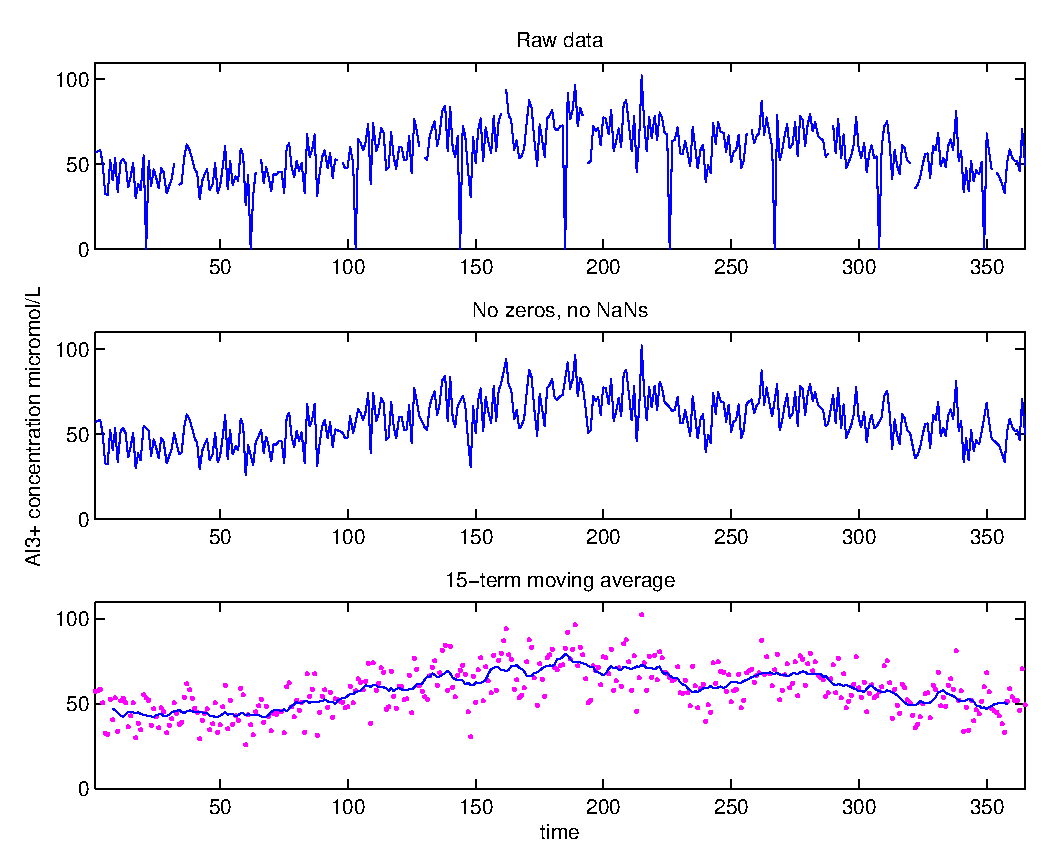
\includegraphics[width=1.0\textwidth]{./../eps/aluminum-concentration.eps}
  \caption{End result of Project \ref{pr:aluminum-toxicity}.}\label{fig:aluminum-concentration}
\end{figure}


\chapter{Importing data}
\thispagestyle{fancy}
\label{ch:importing-data}
The data files you have used until now consisted mainly of numeric data. However, data is usually a mixture of both text and numeric content. Because of this, it is often not possible to use the {\tt load} command to load these files into the \MATLAB{} workspace. However, as long as the mixed data has a fixed format, \MATLAB{} can make data available for calculation using the function {\tt textread}.

\begin{action} 
Set your work directory to `\textbackslash{}ch11\_importing\_data' and take a look at the contents of the `soildata.txt' file.
\end{action}
\begin{lstlisting}[language=TeX]
testfile for textread
J.H. Spaaks & P.Kraal

soil profile       : A234.3
date               : 15-Sep-2003

soil horizon       : nominal class - FAO classification
depth              : depth of top of soil horizon
thickness          : thickness of soil horizon
root density class : 1=very high,2=high,3=intermediate,
                     4=low,5=very low,6=no roots

soil horizon    depth    thickness    root density class
[-]             [m]      [m]          [m/m3]	
Ah, 0,  0.15,  1
Bs, -0.15,    0.18,  3
Bt, -0.33,  0.09,  5
1C, -0.42,       2.07, 5
\end{lstlisting}
At first glance, this file doesn't seem to have a fixed format. Yet it does: the first 11 lines contain the description of the data, line 12 is empty, line 13 contains the variable names, line 14 the units, and lines 15 to 18 consist of the data itself with a comma to separate fields. This formatting enables us to load the file into \MATLAB{} with {\tt textread}\index{textread@\texttt{textread}}. In its simplest form, {\tt textread} expects the following syntax:
\begin{lstlisting}[numbers=none]
[A,B,C] = textread('filename','format')
\end{lstlisting}
where {\tt A}, {\tt B} and {\tt C} are the variables in which the data from the fields of {\tt \squote{filename}} will be stored, and {\tt \squote{format}} is a character array (see Table~\ref{tab:array-classes} on page~\pageref{tab:array-classes}}) in which you specify how you want \MATLAB{} to interpret the data from {\tt \squote{filename}}. The format string\index{format string} is composed of smaller parts, each of which must start with the {\tt \%} sign. Each of the parts has the same structure: after the {\tt \%} sign, there can be an optional number, followed by a letter indicating how you want \MATLAB{} to interpret the information that you are reading (see Table~\ref{tab:format-string-values}).
\begin{table}[ht]
\vspace{1em}
\caption{Format string values.}
\label{tab:format-string-values}
\vspace{-0.25em}
\centering
\begin{tabular}{|c|l|}
\hline
\textbf{Format string}&\textbf{Description}\\
\hline
{\tt d}&Reads an integer value\\
\hline
{\tt f}&Reads a floating point value\\
\hline
{\tt c}&Reads a character value\\
\hline
\end{tabular}
\end{table}
At this point, the usage of {\tt textread} is probably still rather vague, so let's take a look at an example. The correct syntax for extracting the data from `soildata.txt' is listed in \lstlistingname~\ref{list:textread-example}.
\lstinputlisting[numbers=none,float=ht,caption={Example of {\tt textread}. Note that {\tt \squote{...}} breaks the command line for easier reading and printing.},label={list:textread-example}]{./../m/read_soildata.m}\index{...@\texttt{...}}
This way, you can tell \MATLAB{} from which file it needs to read ({\tt \squote{soildata.txt}}), and which format it should use ({\tt \squote{\%2c\%f\%f\%d}}). With this format string, you subsequently read 2 characters, a floating-point, another floating-point, and an integer, before \MATLAB{} goes on with the next line. Because there are 4 {\tt \%} signs, there must also be 4 variables: {\tt {[Hor,D,Th,RtDns]}}. If at this point we would try to read the data with:
\begin{lstlisting}[numbers=none]
[Hor,D,Th,RtDns] = textread('soildata.txt','%2c%f%f%d')
\end{lstlisting}
\MATLAB{} would raise an error, because it will start to read at the very first line of the file unless you specify where to start. This is why the parameter {\tt \squote{headerlines}}\index{`headerlines@\texttt{\squote{headerlines}}} was included in \lstlistingname~\ref{list:textread-example}: it tells \MATLAB{} how many lines need to be skipped before the format string can be applied. For the case of `soildata.txt', there are 14 headerlines that need to be skipped, hence the {\tt 14} directly after {\tt \squote{headerlines}}. Note that we are no longer using {\tt textread} with:
\begin{lstlisting}[numbers=none]
[A,B,C] = textread('filename','format')
\end{lstlisting}
but instead we are using the form with which you can pass options, or as they are formally known `parameter/value pairs'\index{parameter/value pairs}:
\begin{lstlisting}[numbers=none]
[A,B,C] = textread('filename','format',parameter1,value1,...
                                       parameter2,value2)
\end{lstlisting}
In the same way as we are assigning the value 14 to the parameter {\tt \squote{headerlines}}, we can specify the column delimiter symbol by means of the {\tt \squote{delimiter}}\index{`delimiter@\texttt{\squote{delimiter}}} parameter. For the case of `soildata.txt', the column delimiter symbol is set to the comma sign {\tt \squote{,}}. Besides {\tt \squote{headerlines}} and {\tt \squote{delimiter}}, {\tt textread} has a lot more functionality to offer. For further information, including some examples, you can consult the {\tt doc} function. 
\begin{action}
Make sure you understand the {\tt textread} example above, especially the way in which the format string is used. Now try to insert an asterisk somewhere in the format string, to ignore one of the fields from `soildata.txt' (Refer to the documentation on how to use this asterisk). Remember that the number of fields you are trying to read must be equal to the number of output arguments, otherwise \MATLAB{} will raise the error below:
\end{action}
\begin{lstlisting}[numbers=none]
??? Number of outputs must match the number of unskipped input fields.
\end{lstlisting}
\begin{action}
Now that you have practiced a little, it's time to try something more ambitious. Open `knmi\_dh.txt'\footnote{Data from \url{www.knmi.nl}}. This file contains information on 14 meteorological parameters monitored from 01-Jan-2001 to 12-Aug-2003 in Den Helder, The Netherlands (station number 235; see excerpt on page~\pageref{list:knmi_dh}). Use {\tt textread} to load the prevailing wind direction (DDVEC) into the \MATLAB{} workspace as {\tt WDirDeg}. For the moment, let you command ignore all columns other than DDVEC.
\end{action}
\begin{action}
Use the function {\tt conv\_deg2rad} (see page~\pageref{lab:conv_deg2rad}) to create a vector {\tt WDirRad} with {\tt DDVEC} in radians. In order to use the function, copy it to your work directory.
\end{action}
\begin{action}
Plot {\tt WDirRad} using the {\tt rose}\index{rose@\texttt{rose}} function. Consult the documentation for details. Add a title.
\end{action}
\begin{action}
Make an additional figure in which you visualize rose diagrams for January and July using subplots. Limit yourself to the years 2001 and 2002. Use logical arrays and {\tt find} to make your selections. You may want to alter your {\tt textread} format string to also read the dates that a particular measurement was taken.
\end{action}
\begin{action}
Choose three variables from the KNMI data set that you find interesting. Write a program that reads these data from the KNMI file and visualizes them in the way most suitable for the type of data displayed.
\end{action}

\begin{landscape}
\lstinputlisting[firstline=1,lastline=45,float=p,language=TeX,nolol,label={list:knmi_dh}]{./../m/knmi_dh.txt}
\end{landscape} % add knmi figures
\chapter{More projects}
\thispagestyle{fancy}
\label{ch:more-projects}


\project{Reisdorf river dam}
\label{pr:reisdorf}
To obtain a reliable source of drinking water and energy, the river S\^{u}re was dammed near Esch-sur-S\^{u}re during the 1960s. The resulting Lake of the Upper S\^{u}re is now one of the most popular vacation spots in Luxembourg. The successful exploitation of this artificial lake has persuaded the city council of Reisdorf to construct a dam of their own. They expect that the fresh water, energy and flourishing tourist industry will bring them health and wealth. The city council has asked a team of experts from the University of Amsterdam to research the consequences of the erection of such a dam. In this exercise, we will simulate the flooding of the Ernz Blanche river valley.
\begin{action}
Set your work directory to the folder `\textbackslash{}ch12\_more\_projects\textbackslash{}proj06\_reisdorf'. 
\end{action}
\begin{action}
Load the files into the workspace using:
\end{action}
\lstinputlisting[numbers=none,nolol]{./../m/load_ebd.m}
\begin{action}
Visualize the Ernz Blanche DEM. 
\end{action}
\begin{action}
The file `dam\_height.txt' contains data on the dimensions and location of the dam. Visualize the dam by using {\tt imagesc}, then use the zoom-in feature to inspect the top rows where the Ernz Blanche leaves the map. The correct surface elevation data -after construction of the dam- is obtained by adding the values in {\tt DamHeight} to {\tt EBD}.  
\end{action}
To analyze the consequences of the dam, you need to have insight in the water input into the system. Based on historical data, we have a dataset (`ebsupply.txt') with the volumes of water [m$^{3}$] that will flow into the lake each month once the dam is closed. 
\begin{action}
Visualize the data from `ebsupply.txt'.
\end{action}
The first 3 years after construction, the dam is kept closed to allow the water level to rise behind the dam for a profitable dam discharge.
\begin{action}
Calculate the volume of water that has accumulated behind the dam in these 3 years.
\end{action}
We would like to know which area is flooded after these three years.
\begin{action}
Why is it not possible to calculate the water level directly from the water volume?
\end{action}
In contrast to the difficulty in calculating the water level from the water volume, the reverse problem is quite easy: suppose you would know the water level {\tt h}, the grid cell dimensions and the grid cell elevation (the DEM), it would be relatively easy to calculate the water volume beneath this water level. In this exercise, we will exploit this to approximate the true water level. A function has already been created that calculates water volume under a given water height, but accidentally it was messed up. The command lines are intact, but the order is wrong. The code can be found in the file `mess.txt'.
\begin{action}
Put the lines in `mess.txt' in the right order and save the file as `\starred{name}\_calcvol.m' (with your last name for \starred{name}). Refer to Chapter~\ref{ch:functions} if you forgot how a function is structured.
\end{action}
\hintbox{Variables that occur after the `='-sign must have been assigned previously; new variables can only occur before the `='-sign.}
\begin{action}
To test if you changed the order of the lines correctly, type
\prompt{sum(sum(calcvol(241.1318,EBD+DamHeight,25,25)))}
(don't forget to add your last name to the function call). This should return 1.0000e+007.
\end{action}
\begin{action}
If {\tt h}, {\tt CellSizeX} and {\tt CellSizeY} are in meters, what are the units of this result?
\end{action}
To be able to assess which grid cells of the DEM are flooded by the water in the lake after three years, you need to calculate the water level (above sea level) given the calculated water volume. Since it is not possible to calculate {\tt h} directly, you must use an approximation method. This approximation method is used to try out a number of assumed water levels. For each assumed water level, you can calculate the water volume that is associated with it using {\tt calcvol}. The water volume that is associated with the assumed water level is then compared to the actual water volume of the lake (which we can get from the values in {\tt EBSupply}). If the assumed volume is too low, we need to adjust the assumed water level upward; if the assumed water volume is too high, we need to adjust the assumed water level downward. With each adjustment, the interval containing the true water level decreases. We need to keep adjusting until the interval has become sufficiently small. An efficient way for adjusting the value of water level is the so-called 'bisection method'\index{bisection method}. The first step of the bisection method is to define the \textul{initial} lower {\tt hLo} and upper {\tt hUp} bounds on the water level. At any point during the approximation, the interval [{\tt hLo},{\tt hUp}] is as small as possible, given the knowledge that has been collected so far about the true water level {\tt hAct}.
\begin{action}
Determine the lowest (bottom of the lake) and highest (maximum height in the DEM) water levels. These values form the initial estimates of {\tt hLo} and {\tt hUp} (\textit{Step 1}, see Figure~\ref{fig:water-levels}).
\end{action}
\begin{action}
{\tt hMid} is defined as the average of {\tt hLo} and {\tt hUp}. Calculate the corresponding water volume with {\tt calcvol} (\textit{Step 2}, see Figure~\ref{fig:water-levels}).
\end{action}

\noindent The actual water volume is either between the volume associated with {\tt hLo} and {\tt hMid}, or between {\tt hMid} and {\tt hUp}, meaning that the actual water level is also in that interval. Since you now know whether the actual water level {\tt hAct} is in the lower part or the upper part, you eliminate the part that does not contain {\tt hAct} by redefining either {\tt hLo} or {\tt hUp} (\textit{Step 3}, see Figure~\ref{fig:water-levels}).

\noindent In Step 3 of the figure, {\tt hLo} remains unchanged with respect to its position in Step 2, whereas the former {\tt hMid} (see Step 2) is now defined as {\tt hUp}, since you found out that the actual {\tt hAct} is certainly not in the Step 2-interval [{\tt hMid},{\tt hUp}]. Steps 2 and 3 are repeated until the interval [{\tt hLo},{\tt hUp}] has become small enough to meet your preset criterion.

\begin{action}
Finish Figure~\ref{fig:water-levels} by drawing lines in the lower right subplot. Assign each line a label {\tt hLo}, {\tt hMid}, and {\tt hUp}.
\end{action}

\begin{figure}[htbp]
  \centering
    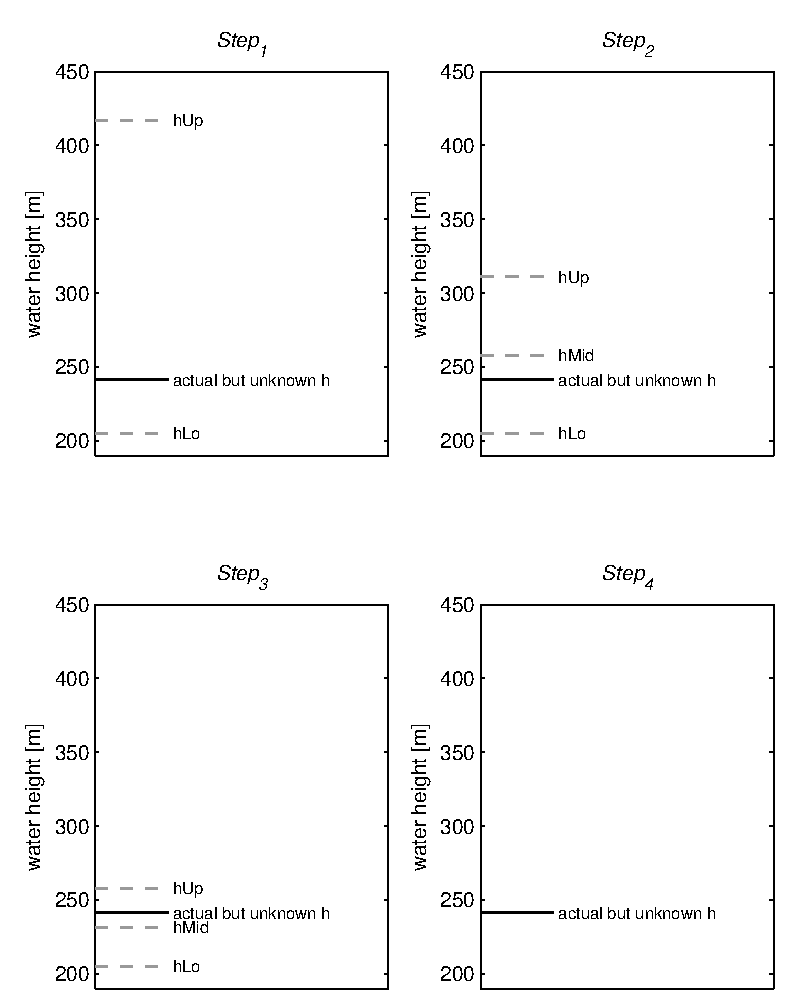
\includegraphics[width=1.0\textwidth]{./../eps/water-levels.eps}
  \caption{Graphical demonstration of the bisection method.}
  \label{fig:water-levels}
\end{figure}


\noindent In the next few exercises, you will implement the bisection technique in a function that can be used to approximate the actual water level associated with a given water volume behind the dam. This function is subsequently used to approximate the water depth of the lake for each month during the first three years after the dam was erected. The function that you will be developing uses the function {\tt calcvol} that you already made.


\begin{action}
First think of the input variables that you need and the output that you want. Together this determines the function call.
\end{action}
\begin{action}
A rough setup of the program is given in the function m-file `outline.m'. Save this file as `\starred{name}\_approxh.m' (where \starred{name} is your last name) and edit this file until it produces the right result as shown in Figure~\ref{fig:lake-reisdorf-36-months}.
\end{action} 

\begin{figure}[htbp]
  \centering
    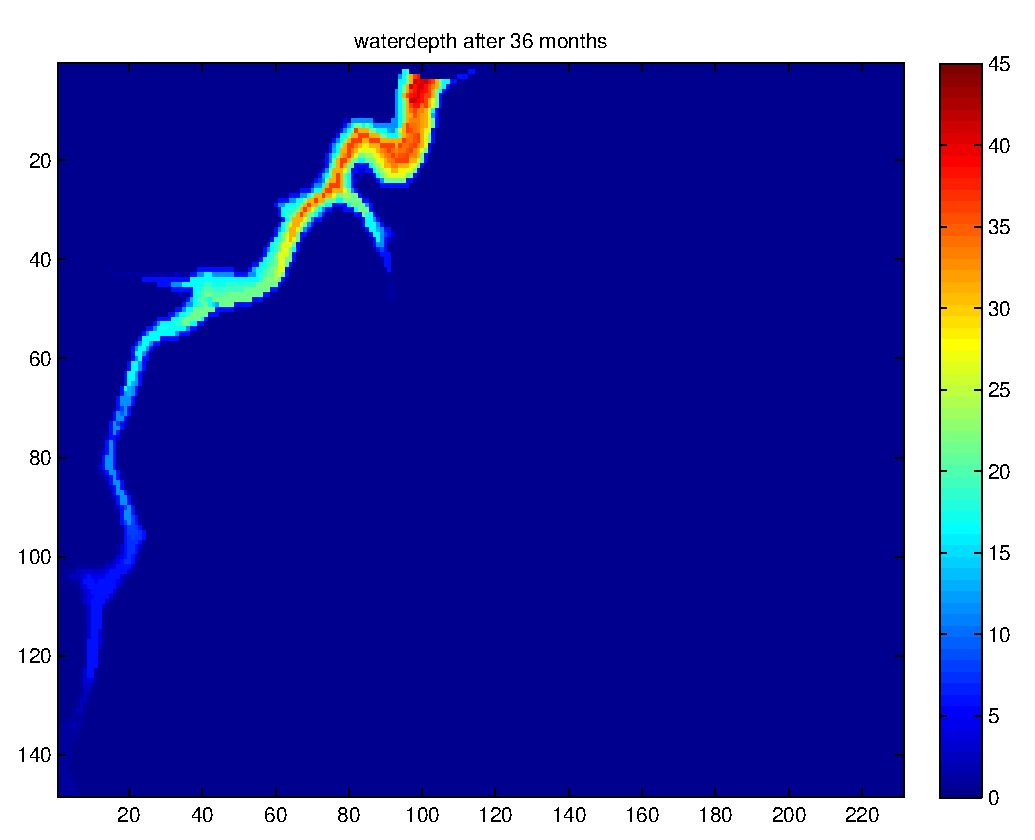
\includegraphics[width=0.75\textwidth]{./../eps/lake-reisdorf-36-months.eps}
  \caption{Distribution of water depths 36 months after the dam was closed.}
  \label{fig:lake-reisdorf-36-months}
\end{figure}

\noindent We are not only interested in the inundated area after three years, but we would like to know the inundated area for each month after the closure of the dam and as long as the water level has not reached the upper level of the dam.

\begin{action}
Start a new script called `\starred{name}\_reisdorf.m' (with your last name for \starred{name}). Let your script visualize the water depth in the valley for each month after the closure of the dam, starting from the dry situation and continuing until the valley is filled up to the upper level of the dam. Use the {\tt approxh} function and the {\tt calcvol} function that you have already written.
\end{action}

\noindent So far, we have used {\tt imagesc} in its simplest form: {\tt imagesc(X)}. This form visualizes the array {\tt X} using a gradient of colors. The colors are automatically set in such a way that they range from the minimium of {\tt X} to the maximum of {\tt X}. However, sometimes you want to set these color limits yourself. For this, you can use {\tt imagesc} with a second input argument: {\tt imagesc(X,C)}\index{imagesc@\texttt{imagesc}}, where {\tt C} is a 1x2 numeric variable, with the user-specified color limits. For instance, in the Reisdorf example of Figure~\ref{fig:lake-reisdorf-36-months}, the minimum color has been set to 0, whereas the maximum color has been set to 45. The command to do this is: {\tt imagesc(WaterDepth2D,[0,45])}.

\begin{action}
Use the 2-argument form of {\tt imagesc} to set the color limits on your water depth figure.
\end{action}

\section{Making movies}
\index{movie}
Extensive calculation results often ask for some kind of animated output. For example, the filling of the reservoir could be visualized as a function of time. In this section you learn how you can save these animations\index{animation} in movies that can be shown without having to run the \MATLAB{} program again.

\noindent A movie consists of frames\index{frame}, just like a traditional celluloid movie. You need to initialize the movie by including the following line in the initialization part:
\begin{lstlisting}[numbers=none]
aviObj = avifile('testmovie.avi','fps',5,...
                         'compression','none');
\end{lstlisting}\index{avifile@\texttt{avifile}}

\noindent This example initializes a movie file `testmovie.avi'. Using the {\tt \squote{fps}}\index{`fps@\texttt{\squote{fps}}} (for `frames per second') option, you can specify at what speed you want to play the movie later. In the example, a frame rate\index{frame rate} of 5 frames per second\index{frames per second} is used. Furthermore, you can specify the compression algorithm that \MATLAB{} will use. For now, we will set {\tt \squote{compression}}\index{`compression@\texttt{\squote{compression}}} to {\tt \squote{none}}, but we will return to this later in Section~\ref{ch:compression}. Running the above command will create a variable {\tt aviObj} of data class `avifile object'. (You can check this in the workspace). See {\tt doc avifile} for more details.

\noindent After the avifile object has been initialized, you can add as many frames as you like (as long as there is available space on your harddisk). After issuing the visualization commands (such as {\tt imagesc}, {\tt scatter}, {\tt surf} or {\tt plot}), you need to capture\index{capture} the frame and add it to your avifile object variable. A generic structure of a script that creates a movie is included in \lstlistingname~\ref{list:generic-moviecapture}.
\lstinputlisting[float,label={list:generic-moviecapture},caption={Generic structure of a script that creates an *.avi\index{*.avi file extension} movie.}]{./../m/generic_moviecapture.m}

\subsection{On the need for closure}
It is crucial that your program gets to closing the avifile object. If you forget to include this part, or if the program crashes before it gets to closing the avifile, you end up with an *.avi file (in this case `testmovie.avi') which cannot be played. This is because media players will wait for \MATLAB{} to release its handle on the file (which it never will, since the program crashed). If this is the case, you need to issue a {\tt clear all}\index{clear all@\texttt{clear all}} \textit{at the prompt}. Note that you will generally not include the {\tt clear all} in your script, since it makes debugging impossible. For this course, we will \textit{only} use {\tt clear all} when dealing with movies that have not been finalized. In all other situations, you need to use {\tt clear}.
\begin{action}
Change your program in such a way that it creates a movie of the filling of the artificial lake for each month for the first 3 years. 
\end{action}

\begin{action}
Re-read the part about {\tt for}-loops and {\tt while}-loops on page \pageref{sec:for-loops}--\pageref{sec:while-loops}. Now change your script in such a way that it keeps calculating the monthly water depth map for as long as the water level is lower than the level of the dam.
\end{action}


\subsection{Compression}
\label{ch:compression}
As you may have noticed, making a movie without using any compression can generate big files, especially when you are capturing many frames. This is where compression algorithms come in handy. Compression algorithms, or codecs\footnote{\url{http://en.wikipedia.org/wiki/Codec}}\index{codec}, are used to decrease file size, while maintaining as much of the original quality as possible. In this respect, they are similar to what MP3 is for audio, what JPEG is for photos, or what ZIP is for data. Codecs are well worth looking into, because a good codec can decrease a file by a factor 100 without compromising the movie quality!

\begin{action}
In your work directory, there is a codec file `mpg4c32.dll', which can be used to compress your movie file. In order for this to work, you need to set the {\tt \squote{compression}} option to {\tt \squote{mpg4}}. Make the necessary changes to have your program use this compression algorithm. 
\end{action}



\projectfooter{}



\project{Flow path}
The characteristics of a drainage network play a great part in determining how water moves through a basin and consequently affects issues such as water quality and quantity (including flooding). Drainage patterns dramatically affect people and the environment downstream regardless of administrative borders, often over long distances, and on a very large scale with long-lasting implications. 

In this project, you will analyze water movement in a drainage basin. You will develop a program that calculates the pathway of water for a given DEM, from an arbitrarily chosen starting point to the lowest point of the landscape.
\begin{action}
Set your working folder to `\textbackslash{}ch12\_more\_projects\textbackslash{}proj07\_flowpath', start a new script called `\starred{name}\_flowpath.m' (with your last name for  \starred{name} ) and visualize `valleydem.txt'.
\end{action}
\begin{action}
If you would drop a ball in {\tt valleydem(10,4)}, where would it end up?
\end{action}
To determine water movement in this area, you can use the principle of `steepest descent': this principle is based on the assumption that water movement between cells is driven by the maximum gradient between the origin cell and its 8 surrounding cells.

In order to calculate this maximum gradient, you need to know the difference in height between the origin cell and the surrounding cells ({\tt DeltaH}) and the distance from the surrounding cells to the origin cell ({\tt Dist}). These distances are not all equal.
\begin{action}
Given that the cell dimensions are 25 x 25m, fill the array below with the distances.
\end{action}

\begin{equation}
\mathtt{Dist} = \left[
\begin{array}{ccc}
\ldots&\ldots&\ldots\\
\ldots&0&\ldots\\
\ldots&\ldots&\ldots\\
\end{array}
\right]
\end{equation}
Do you think that you could now write a script to calculate the path water follows from some given starting point to the lowest point? If so, try it. Start with making a design first and then write your program.
If you don't think you can do it just yet, follow the guidelines below.
\begin{action}
What would be the statement to select a 3x3 submatrix {\tt H} from {\tt valleydem} if the position of the center cell in {\tt H} corresponds with {\tt valleydem(68,55)}? If your command is correct, {\tt H} should be equal to:
\end{action}
\begin{verbatim}
 H =
     113.8968  111.6601  109.4644
     115.4084  113.1661  110.9636
     116.9417  114.6987  112.4948
\end{verbatim}
\begin{action}
Create a 3x3 array {\tt DeltaH} with the height differences between the cells and the center cell.
\end{action}
\begin{action}
Create a 3x3 array {\tt Grad} containing the gradients between the origin cell and its neighbors. The gradient is difference in height divided by distance. 
\end{action}
\begin{action}
Set the value of the center cell in {\tt Grad} to 0 to avoid calculation complications with NaN. If you do not want the warning\index{warning@\texttt{warning}} message in your screen, include the following line in your program, just before the line that causes the warning:
\begin{lstlisting}[numbers=none]
warning('off','MATLAB:DivideByZero')
\end{lstlisting}
Remember that divide-by-zero warnings serve a purpose, so make sure you turn them back on after the line that raises the warning. You can do this by:
\begin{lstlisting}[numbers=none]
warning('on','MATLAB:DivideByZero')
\end{lstlisting}
\end{action}
\begin{action}
If one of the gradients in {\tt Grad} is negative, what does that mean?
\end{action}
Now you have a 3x3 array with the values of the gradients of the surrounding 8 cells. The steepest descent-theory states that water flows (only) in the direction of the cell that has the lowest (most negative) gradient. So, the next step is to determine which of the surrounding cells will be the one into which the water flows.
\begin{action}
Create a 3x3 logical array {\tt LocMin} with value 1 on the position where {\tt Grad} has its minimum value.
\end{action}
\begin{action}
Determine the subscripts of the minimum value within {\tt Grad}. Call them {\tt r} and {\tt c}, respectively.
\end{action}
Keep in mind that the location {\tt [r,c]} is the position of the minimum value in {\tt Grad}, not in {\tt valleydem} (see also Figure~\ref{fig:valleydem-grid}).


\begin{figure}[htb]
  \centering
    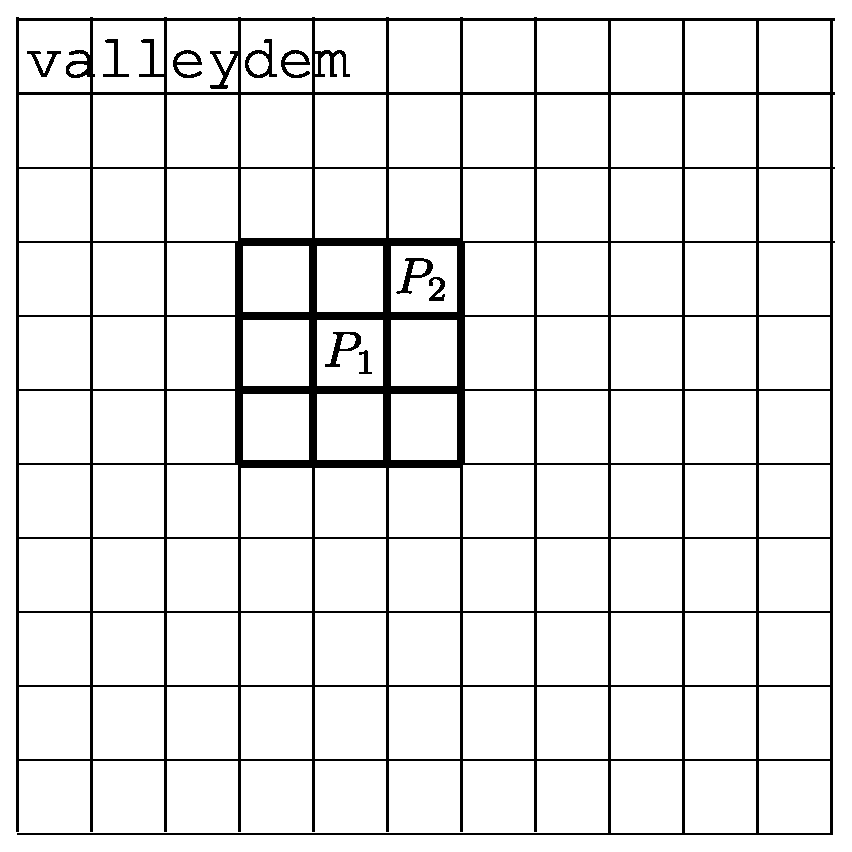
\includegraphics[width=0.5\textwidth]{./../eps/valleydem-grid.eps}
  \caption{The position of {\tt H}, {\tt Dist}, {\tt Grad} within {\tt valleydem}. $P_1$ is the center cell of {\tt H}, {\tt Dist}, and {\tt Grad}, with subscripts r=2 and c=2. The same position in {\tt valleydem} is indicated by ({\tt CurrentRow,CurrentCol}). Position $P_2$ is the position for which the gradient is most negative, i.e., the direction of steepest descent.}
  \label{fig:valleydem-grid}
\end{figure}


\begin{action}
What is the range of valid values for {\tt r}? And for {\tt c}?
\end{action}

\begin{action}
If $P_1$ is the position ({\tt 68},{\tt 55}) in {\tt valleydem}, what is the position of $P_2$?
\end{action}


\begin{action}
If $P_1$ is the position ({\tt CurrentRow},{\tt CurrentCol}) in {\tt valleydem}, what is the position of $P_2$?
\end{action}

\begin{action}
We can use the subscripts of $P_2$ (with respect to {\tt Grad}) to determine its position within {\tt valleydem}. Alter your script in such a way that {\tt CurrentRow} and {\tt CurrentCol} are updated based on the value of {\tt r} and {\tt c}.
\end{action}

\noindent At this point, we have all the necessary constituents for repeating the following steps in a for-loop:
\begin{enumerate}
\item From {\tt valleydem}, select the 3x3 subset around the current location;
\item Calculate the location of lowest gradient;
\item Make the location of lowest gradient the current location.
\end{enumerate}

\begin{action}
Implement the above mentioned steps in your script m-file. Refer to the program outline given in \lstlistingname~\ref{list:flowpath-outline} for guidance on how to structure your program. The result of your program should look like Figure~\ref{fig:flowpath-valleydem1}. Use concatenation commands to keep a record of the value of {\tt CurrentRow} and {\tt CurrentCol}.
\end{action}

\lstinputlisting[float=htbp,caption={Design of a script that calculates the flow path of water through a catchment},label={list:flowpath-outline}]{./../m/outline_project7_flowpath.m}\index{hold on@\texttt{hold on}}\index{hold off@\texttt{hold off}}

\begin{figure}[htbp]
  \centering
    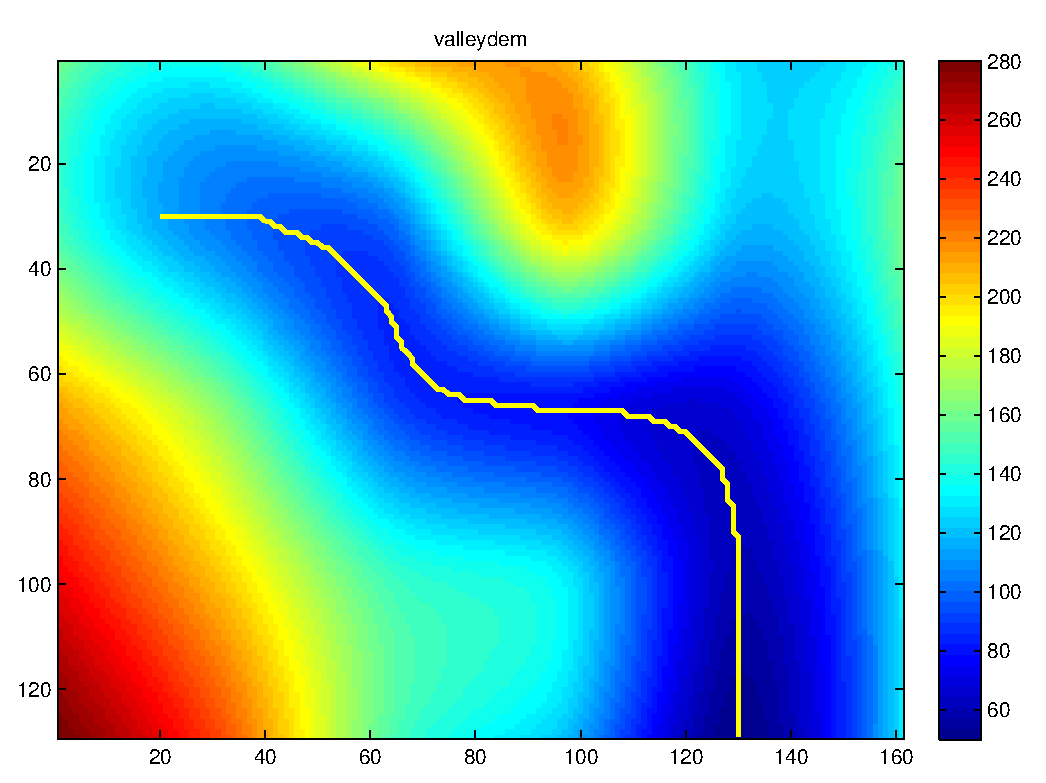
\includegraphics[width=1.0\textwidth]{./../eps/flowpath-valleydem1.eps}
  \caption{Flow path derived from the DEM using the steepest-descent method. Starting point is {\tt valleydem(30,20)}.}
  \label{fig:flowpath-valleydem1}
\end{figure}



\begin{action}
Is it possible to start calculations at position (1,1) of {\tt valleydem}? Why (not)?
\end{action}
At this point, the script m-file calculates the new row and column for 25 iteration steps (see \lstlistingname~\ref{list:flowpath-outline}). However, it is unrealistic that water will stop flowing after 25 steps. What you actually want, is continuous calculation until the borders of the system are reached. 

As opposed to the {\tt for}-loop that performs calculations for a preset number of repetitions, a {\tt while}-loop allows you to perform calculations as long as a certain condition is true. For instance, you could set up a {\tt while}-loop that runs as long as it is {\tt true} that the current position is not on the edge of the domain.

\begin{action}
For which value(s) of {\tt CurrentRow} and {\tt CurrentCol} in {\tt valleydem} can you apply your algorithm? Complete Table~\ref{tab:valleydem-edge}.
\end{action}
\begin{table}[ht]
\caption{While loop conditions}
\label{tab:valleydem-edge}
\centering
\begin{tabular}{|l|p{6cm}|}
\hline
\textbf{Condition}&\textbf{Relational expression in \MATLAB{}}\\
\hline
{\tt CurrentRow} is greater than 1&\ldots\\
\hline
\ldots&\ldots\\
\hline
\ldots&\ldots\\
\hline
\ldots&\ldots\\
\hline
\end{tabular}
\end{table}



\begin{action}
In your script m-file, replace the {\tt for}-loop with a {\tt while}-loop that combines the conditions as stated above.
\end{action}
\begin{action}
Load `valleydem2.txt' and visualize it. Can you see the difference between {\tt valleydem} and {\tt valleydem2}?
\end{action}
\begin{action}
Try to use {\tt valleydem2} in your drainage program (if needed you can stop your program by simultaneously pressing the `Ctrl' and `c' buttons while clicking in the \MATLAB{} command window. 
\end{action}
As you probably found out for yourself, you end up with a never-ending loop because the new DEM contains so-called pits: local minimums. The track ends in a cell with only higher cells surrounding it. You can overcome this by adding an extra condition in your while-statement that tests if the current position is in a pit or not.
\begin{action}
Alter the expression in your while loop in such a way that it tests for pits.
\end{action}
\projectfooter

\pagebreak


\project{Drainage pattern}
\begin{action}
Copy your script m-file from the previous project to the directory '\textbackslash{}chap12\_more\_projects\textbackslash{}proj07\_drainpattern'  and reset your work folder accordingly. Change the script m-file into a function m-file `\starred{name}\_draintrack.m' (with your last name for \starred{name}), with {\tt StartRow}, {\tt StartCol} and {\tt DEM} as input arguments and {\tt Track} as output:
\end{action}
%\vspace{0.5em}
\begin{lstlisting}[numbers=none]
function Track = draintrack(DEM,StartRow,StartCol)
\end{lstlisting}
To get an impression of the total drainage pattern of this valley system, you must run the algorithm for every possible position in {\tt valleydem}. In order to do this, follow the outline below:
\begin{enumerate}
\item Write a script m-file (`\starred{name}\_drainpattern.m'), with a double {\tt for}-loop that calls {\tt draintrack}. 
\item In your {\tt for}-loop, take increments of 10 to avoid long calculation times. 
\item Most of the initial part and the visualization is now not needed in the function and can thus be transported to the main program. Cut and paste as much as possible from the {\tt draintrack} function to the main program. 
\item Check whether the program works well. Use the debugger if necessary.
\end{enumerate}
\begin{action}
Now also try to use the Luxembourg DEM (`demlux.txt') instead of {\tt valleydem}.
\end{action}
As you can see from the error, an analytical error still exists in our program: during calculation, some operations can not be executed because of incorrect variable dimensions. This happens when the program has to deal with more than one lowest gradient and doesn't know which one to use. A relatively easy way to solve this is by always taking the first point.
\begin{action}
Alter your program to always use the first point, even when there are multiple directions with the same lowest gradient. The end result should look like Figure~\ref{fig:drainpattern}.
\end{action}
\begin{action}
The function m-file `randchoosefrom.m' that is present in your directory, lets you pick a value at random if there is more than one direction of steepest descent. Open the function, read the help block, and incorporate it in your script. Note that it's easy to make an analytical mistake here, which will cause your program to calculate an incorrect result (even though it won't raise an error). So think first about what you need to do, before you start implementing.
\end{action}

%\begin{action}
%Can you explain the fact that some drainage directions are crossing each other?
%\end{action}

\begin{action}
Drainage tracks are shorter when the terrain is relatively flat. Why?
\end{action}



\begin{figure}[htbp]
  \centering
    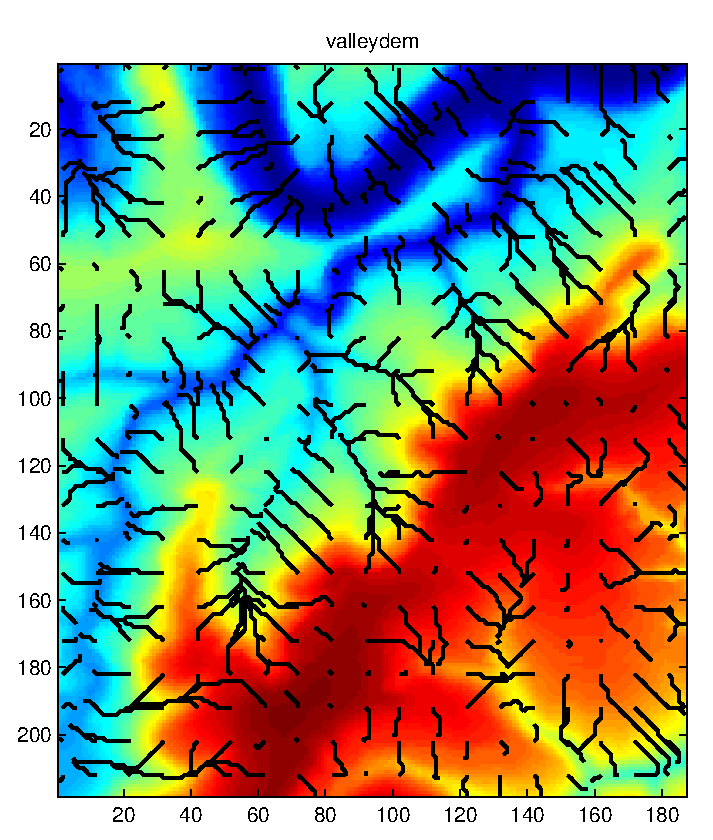
\includegraphics[width=0.75\textwidth]{./../eps/drainpattern.eps}
  \caption{Drainage pattern of the Luxembourg DEM, as determined by the steepest-descent method.}
  \label{fig:drainpattern}
\end{figure}

 
\chapter{External toolboxes}
\thispagestyle{fancy}



\section{User contributed software}
Besides the algorithms that come with the \MATLAB{} program, there is a wealth of user-contributed programs available on the Internet. A good place to look for such programs, is the `File Exchange' on the Mathworks website \url{http://www.mathworks.com/matlabcentral/fileexchange/?sort=downloads}.

\begin{action}
Take 20 minutes to browse through the contents of the File Exchange website. On the left side of the website, there is an item `Files by Category' that you may want to use to limit the search to the `Earth Sciences' domain. 
\end{action}
As you can see, there are many programs available that you can use for free. In this chapter we will use the GoogleEarth Toolbox for \MATLAB{}\index{GoogleEarth Toolbox for MATLAB@GoogleEarth Toolbox for \MATLAB{}}: \url{http://www.mathworks.com/matlabcentral/fileexchange/12954-google-earth-toolbox}. You have a copy of the GoogleEarth Toolbox, located in the folder `pim\_files\textbackslash{}'. In this chapter, you will learn to use the functions in this toolbox.

\project{Google Earth Toolbox}
\label{pr:googleearth}

\section{Installing GoogleEarth}
\begin{action}
Open Windows Explorer and navigate to the folder `pim\_files\textbackslash{}ch13\_toolboxes'. There should be a file `GoogleEarthPerUserSetup.exe'. Click to install the GoogleEarth Viewer.\index{GoogleEarth Viewer}
\end{action}

\section{Setting up the GoogleEarth application}
To avoid problems with displaying and interpreting your GoogleEarth files, it's necessary to have your copy of GoogleEarth set up according to the following specifications:
\begin{enumerate}
\item Click \guitext{Tools} in GoogleEarth's menu and choose \guitext{Options\ldots}. On the tab named \guitext{3D View} check that \guitext{Graphics Mode} is set to \guitext{OpenGL}\index{OpenGL}.
\item On the same tab, set the latitude/longitude format to \guitext{Decimal Degrees} under \guitext{Show Lat/Long}.
\item Also on this tab, set the units of elevation to \guitext{Meters, Kilometers} under \guitext{Show Elevation}.
\end{enumerate}



\section{KML}
The great flexibility of GoogleEarth stems from its use of XML\index{XML}\footnote{\url{http://en.wikipedia.org/wiki/XML}}-based text files, known as KML\index{KML}\index{Keyhole Markup Language}\footnote{\url{http://en.wikipedia.org/wiki/Keyhole_Markup_Language}}-files (you can recognize these files by their extension *.kml\index{*.kml}). Such a file typically contains a series of objects, such as polygons, lines and points. Each of these objects is represented within a KML-file by its KML-tags. For example, we may find a polygon object:
\begin{verbatim}
<Polygon>
...
</Polygon>
\end{verbatim}
Or a line object:
\begin{verbatim}
<LinearRing>
...
</LinearRing>
\end{verbatim}
\vspace{1em}

\noindent Properties such as line width, coordinates, and polygon color may be specified using additional tags. A line may thus be assigned a line style as follows:
\begin{verbatim}
<LineStyle>
   <color>ffffffff</color>
   <width>1.00</width>
</LineStyle>
\end{verbatim}
Which represents a fully opaque, white line of width 1.

\subsection{Automated writing of KML}
Of course, writing KML-tags by manually typing them in a text editor is not practical when working with data containing more than just a few objects. Fortunately though, the task of writing these files can be fully automated using the GoogleEarth Toolbox.

The GoogleEarth Toolbox generates plain ASCII text files. The text contained within these files is formatted according to the Keyhole Markup Language (KML) specification, which allows for a hierarchical organization of the objects and properties contained within the file. KML files can be opened in the GoogleEarth Viewer.

The GoogleEarth Toolbox implements a number of low-level functions for displaying point, line and polygon objects within GoogleEarth. In addition to that, higher-level methods include functions to visualize 2D rasterized data, create contour maps, surface and quiver plots, image overlays (in GIS usually referred to as \textit{draping}), and a few others.

\section{Structure of the GoogleEarth Toolbox}
The core of the toolbox is formed by a set of about 20 \MATLAB{} functions (*.m files) located in the toolbox root folder (`googleearth/'). The majority of these functions generate character arrays in concordance with the KML standard. For each of the m-files, a help file has been included which can be viewed from within the \MATLAB{} help browser. The help files are located in `googleearth/html'. In addition to the help files, demonstrations have been included (`googleearth/demo'). Many of these demos write their output to a separate folder (`googleearth/kml') in order to avoid contaminating directories with files that do not belong there. Folder `googleearth/data' contains additional files such as icon images and Collada models. Folder 'googleearth/doc' contains files pertaining to the printable documentation. Finally, a folder 'googleearth/tmp' has been included, which is used by some functions to write temporary data to. The contents of this folder are automatically emptied by some functions, therefore you should not save important data in it. In fact, it's best if you don't save any file anywhere under `googleearth/'.


\section{Adding the toolbox to the path}
When you use a function name in your scripts or at the prompt, \MATLAB{} starts searching a predefined list (i.e. the `path') of directories where \MATLAB{} functions are stored. 
\begin{action}
At the prompt, type
\prompt{path}\index{path@\textt{path}}
\end{action}
The default list of directories should now be displayed in the command window. In order to use the functions from the GoogleEarth Toolbox, you need to add the toolbox' top-level directory to the path:
\prompt{addpath(\squote{D:\textbackslash{}matlab\textbackslash{}googleearth})}\index{addpath@\texttt{addpath}}
\noindent This will add the indicated directory to the \MATLAB{} search path (see {\tt doc path}). The above command is equivalent to using \guitext{Set Path\ldots} from the \guitext{File} menu of the \MATLAB{} Graphical User Interface. 

\begin{action}
Now type
\prompt{googleearth -docinstall}\index{googleearth@\texttt{googleearth}}
to initialize some files that are needed to use the documentation.
\end{action}
\vspace{1em}
\noindent After adding the toolbox location to the \MATLAB{} path, its functions may be called either from the command window or in scripts. Additionally, the toolbox documentation is accessible through the usual {\tt doc} command. Typing
\prompt{doc googleearth}
\noindent and following the hyperlink will take you to an index page where all functions are listed, along with a short description of their intended usage. As an alternative to using the {\tt doc} command, the documentation may also be accessed by selecting the GoogleEarth item which is now located under \MATLAB{}'s Start button \ding{217} Toolboxes (see Figure~\ref{fig:googleearth-help-menu}). In the documentation files, you can find information on what a particular function does, what variables to pass it, the function's options, links to other functions that perform related tasks, and an example of how the function can be used.


\begin{figure}[!htb]
  \centering
    \fbox{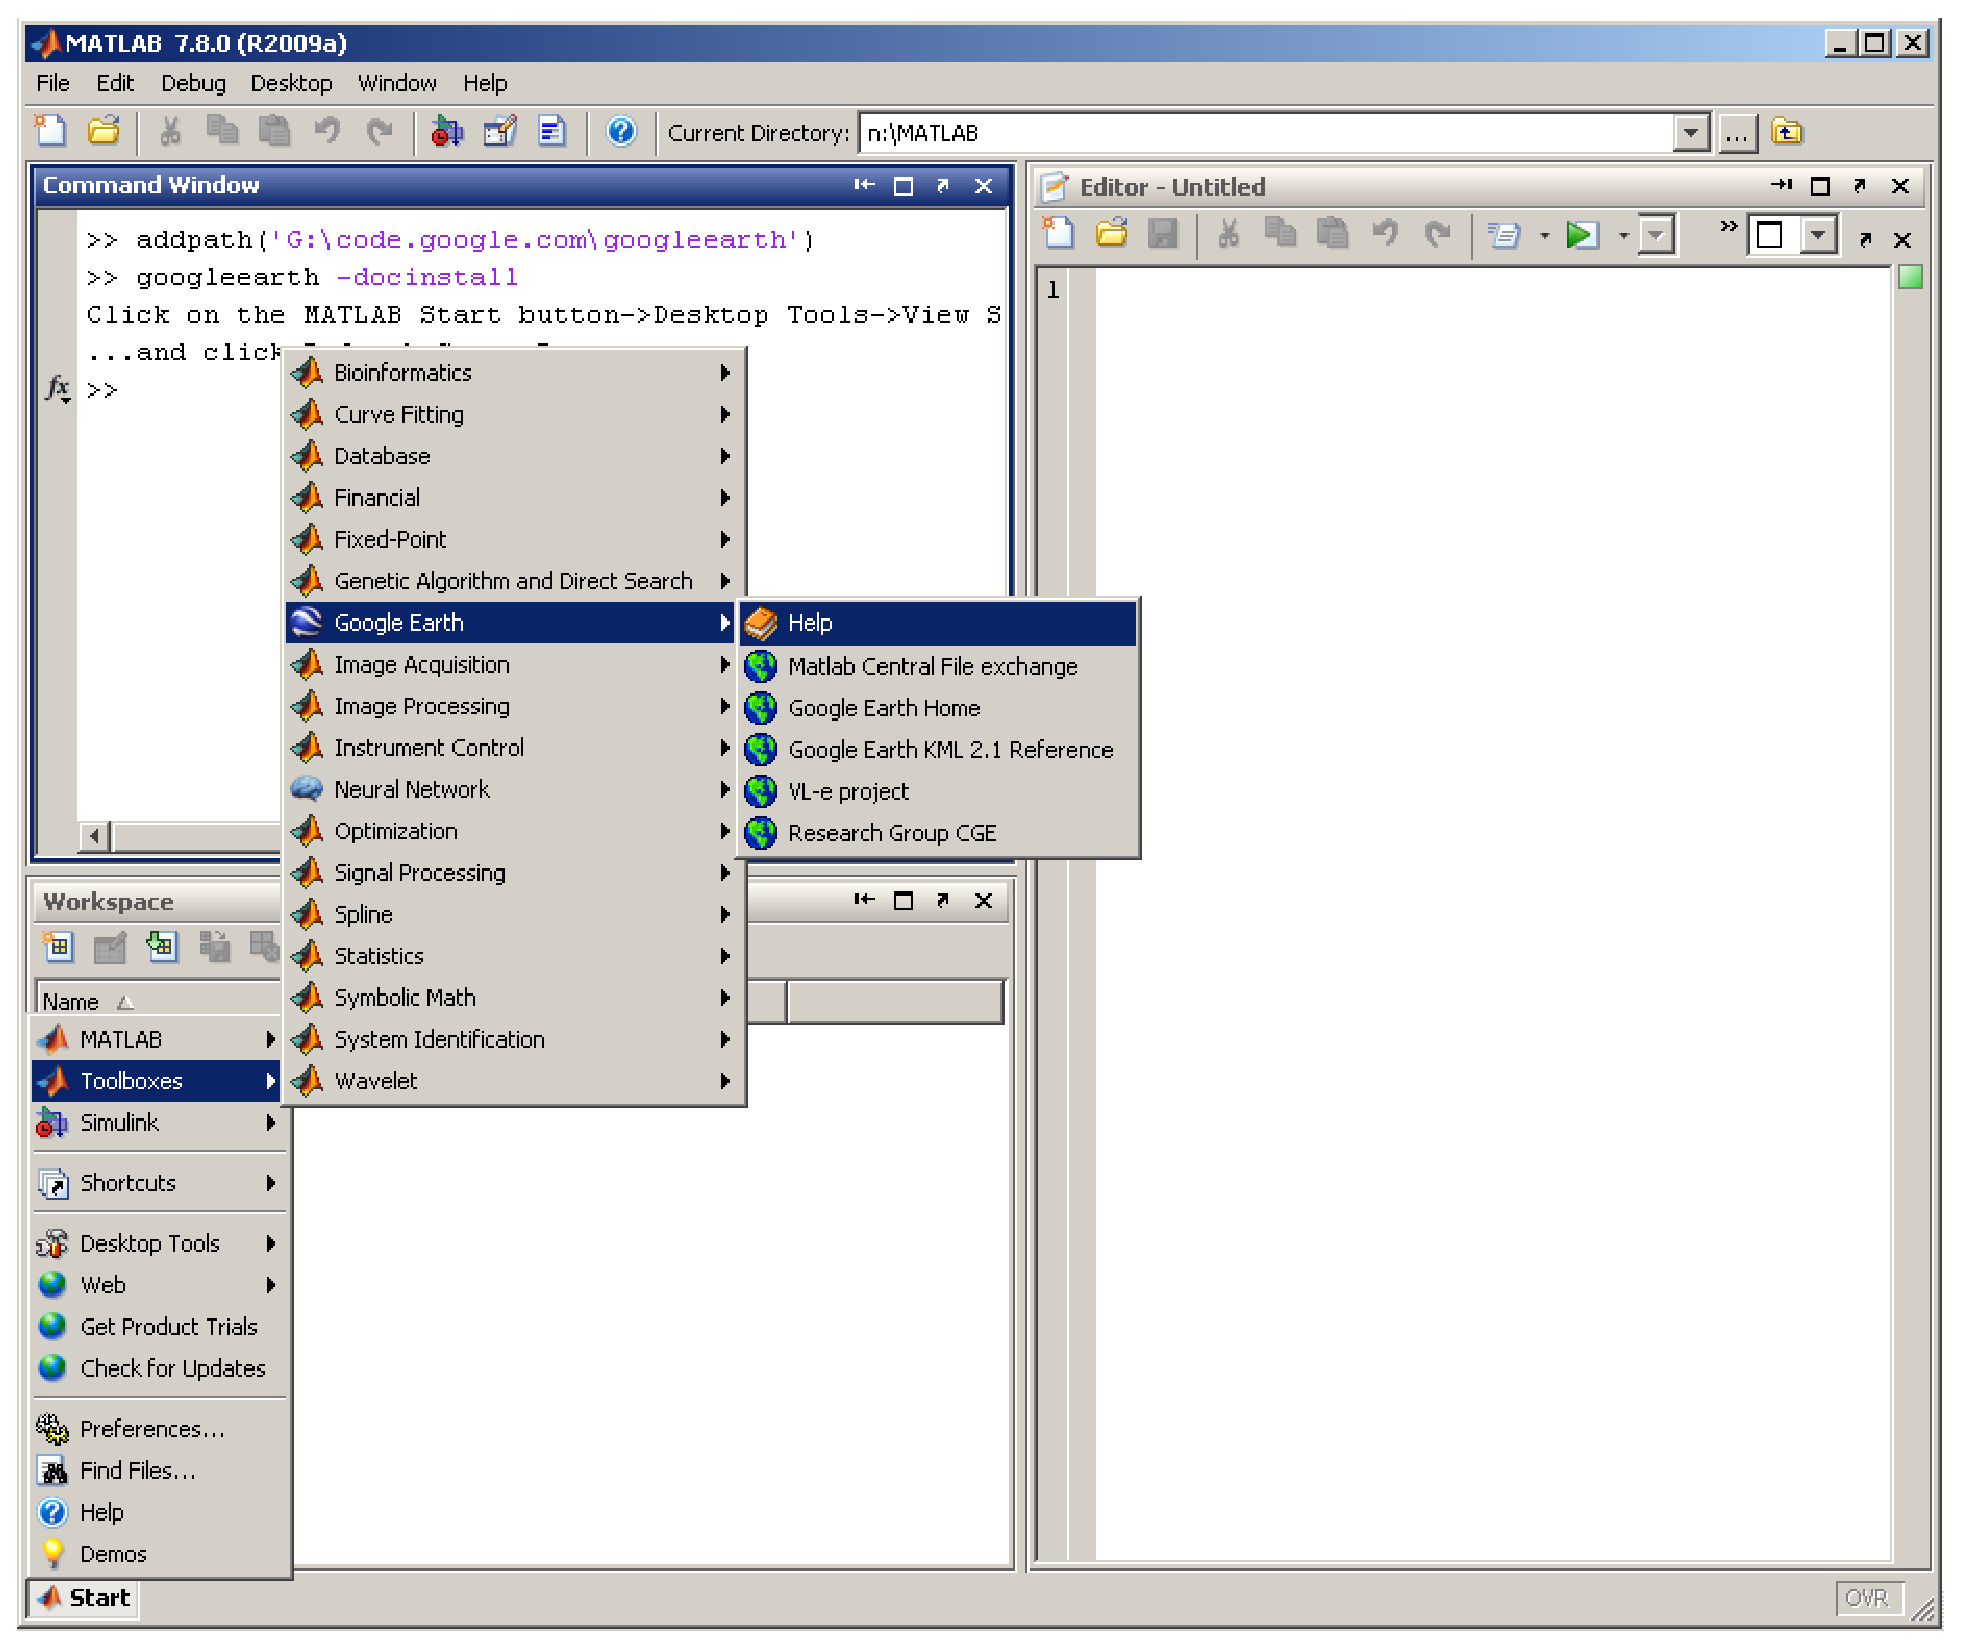
\includegraphics[width=1.0\textwidth]{./../eps/googleearth-help-menu.eps}}
  \caption{Accessing the GoogleEarth Toolbox documentation.}\label{fig:googleearth-help-menu}
\end{figure}







\section{Point features}
\begin{action}
In the GoogleEarth Viewer, go to a location of your choice and write down its latitude and longitude. 
\end{action}

\begin{action}
Navigate to the documentation on {\tt ge\_point}\index{ge\_point@\texttt{ge\_point}} or enter the command below at the prompt:
\prompt{doc ge\_point}
This should invoke the documentation about {\tt ge\_point}. Read through it carefully.
\end{action}

\begin{action}
Begin a new m-file called `\starred{name}\_point.m'. Let the script generate a character array called {\tt kmlStr}, which contains the location of your choice in KML format.
\end{action}
You should now have a character array with KML-formatted text. However, to be able to see your point in the GoogleEarth Viewer, we need to write the character array to a *.kml file.
\begin{action}
Consult the documentation on {\tt ge\_output}\index{ge\_output@\texttt{ge\_output}}, and use it to save your KML-formatted text to a *.kml file. 
\end{action}

\begin{action}
Open your *.kml file in the GoogleEarth Viewer and verify that it shows a point at the location of your choice.
\end{action}

\begin{action}
By default, the point is labeled with the full filename of its *.kml file when opened in the GoogleEarth Viewer (see left-hand pane \guitext{Places}). It's often useful to assign a different name to the object when viewed in GoogleEarth using {\tt ge\_output}'s parameter {\tt \squote{name}}. Change how your point is displayed in the \guitext{Places} pane in the GoogleEarth Viewer.
\end{action}

\begin{action}
Instead of the default placemarker icon, use this {\tt \squote{iconURL}}\index{`iconURL@\texttt{\squote{iconURL}}} (or any other icon of your choice): \url{http://maps.google.com/mapfiles/kml/pal3/icon35.png}.
\end{action}


\section{Line features}
Lesser black backed gulls (\textit{Larus fuscus}) are sea birds that spend spring and summer in The Netherlands but, like some of its human inhabitants, spend their winters in Southern Europe. While migration patterns of sea birds have been monitored before, until now it was not possible to get the detailed information about their movements needed to gain insight into their foraging behavior. Therefore, the University of Amsterdam developed a new flexible tracking system that enables detailed monitoring of the bird's movement. These so-called `GPS-loggers' consist of a tiny GPS system combined with a miniature recording device and transceiver, powered with a solar panel. They weigh only 18 grams, allowing birds to carry them on their backs without being restricted in their movements (see Figure~\ref{fig:lesser-black-backed-gull}). Once attached to the birds, the devices record their position, wing beat frequency, temperature and air pressure during their local and migratory movements with great detail.
In this section, you will use the GoogleEarth Toolbox to visualize the migratory route that gull~\#41745 has taken.
\begin{figure}[!htbp]
  \centering
    \fbox{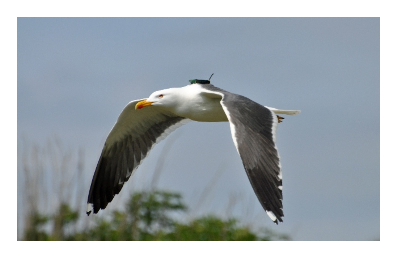
\includegraphics[width=1.0\textwidth]{./../eps/lesser-black-backed-gull.eps}}
  \caption{Lesser black-backed gull (\textit{Larus fuscus}) equipped with a GPS logger (Photo: Cees Camphuysen, NIOZ).}\label{fig:lesser-black-backed-gull}
\end{figure}

\begin{action}
Start a new script `\starred{name}\_seagull.m'. 
\end{action}
\begin{action}
Use {\tt textread} to load the seagull data from the file `pim\_files\textbackslash{}ch13\_toolboxes\textbackslash{}larus-fuscus.txt'. If you are not successful doing this but there's no one around to help you, use {\tt load(\squote{larus-fuscus-cheat.mat})} to read from a binary file, so that you won't waste too much time. (But don't forget to ask about {\tt textread} later).
\end{action}
\begin{action}
Consult the documentation on the use of {\tt ge\_plot}\index{ge\_plot@\texttt{ge\_plot}}, and use it to visualize the bird's track. Adapt the script so that it produces a fully opaque, red line of width 1.5. If you do this correctly, the data should be displayed as in Figure~\ref{fig:larus-fuscus}.
\end{action}
\begin{figure}[!htbp]
  \centering
    \fbox{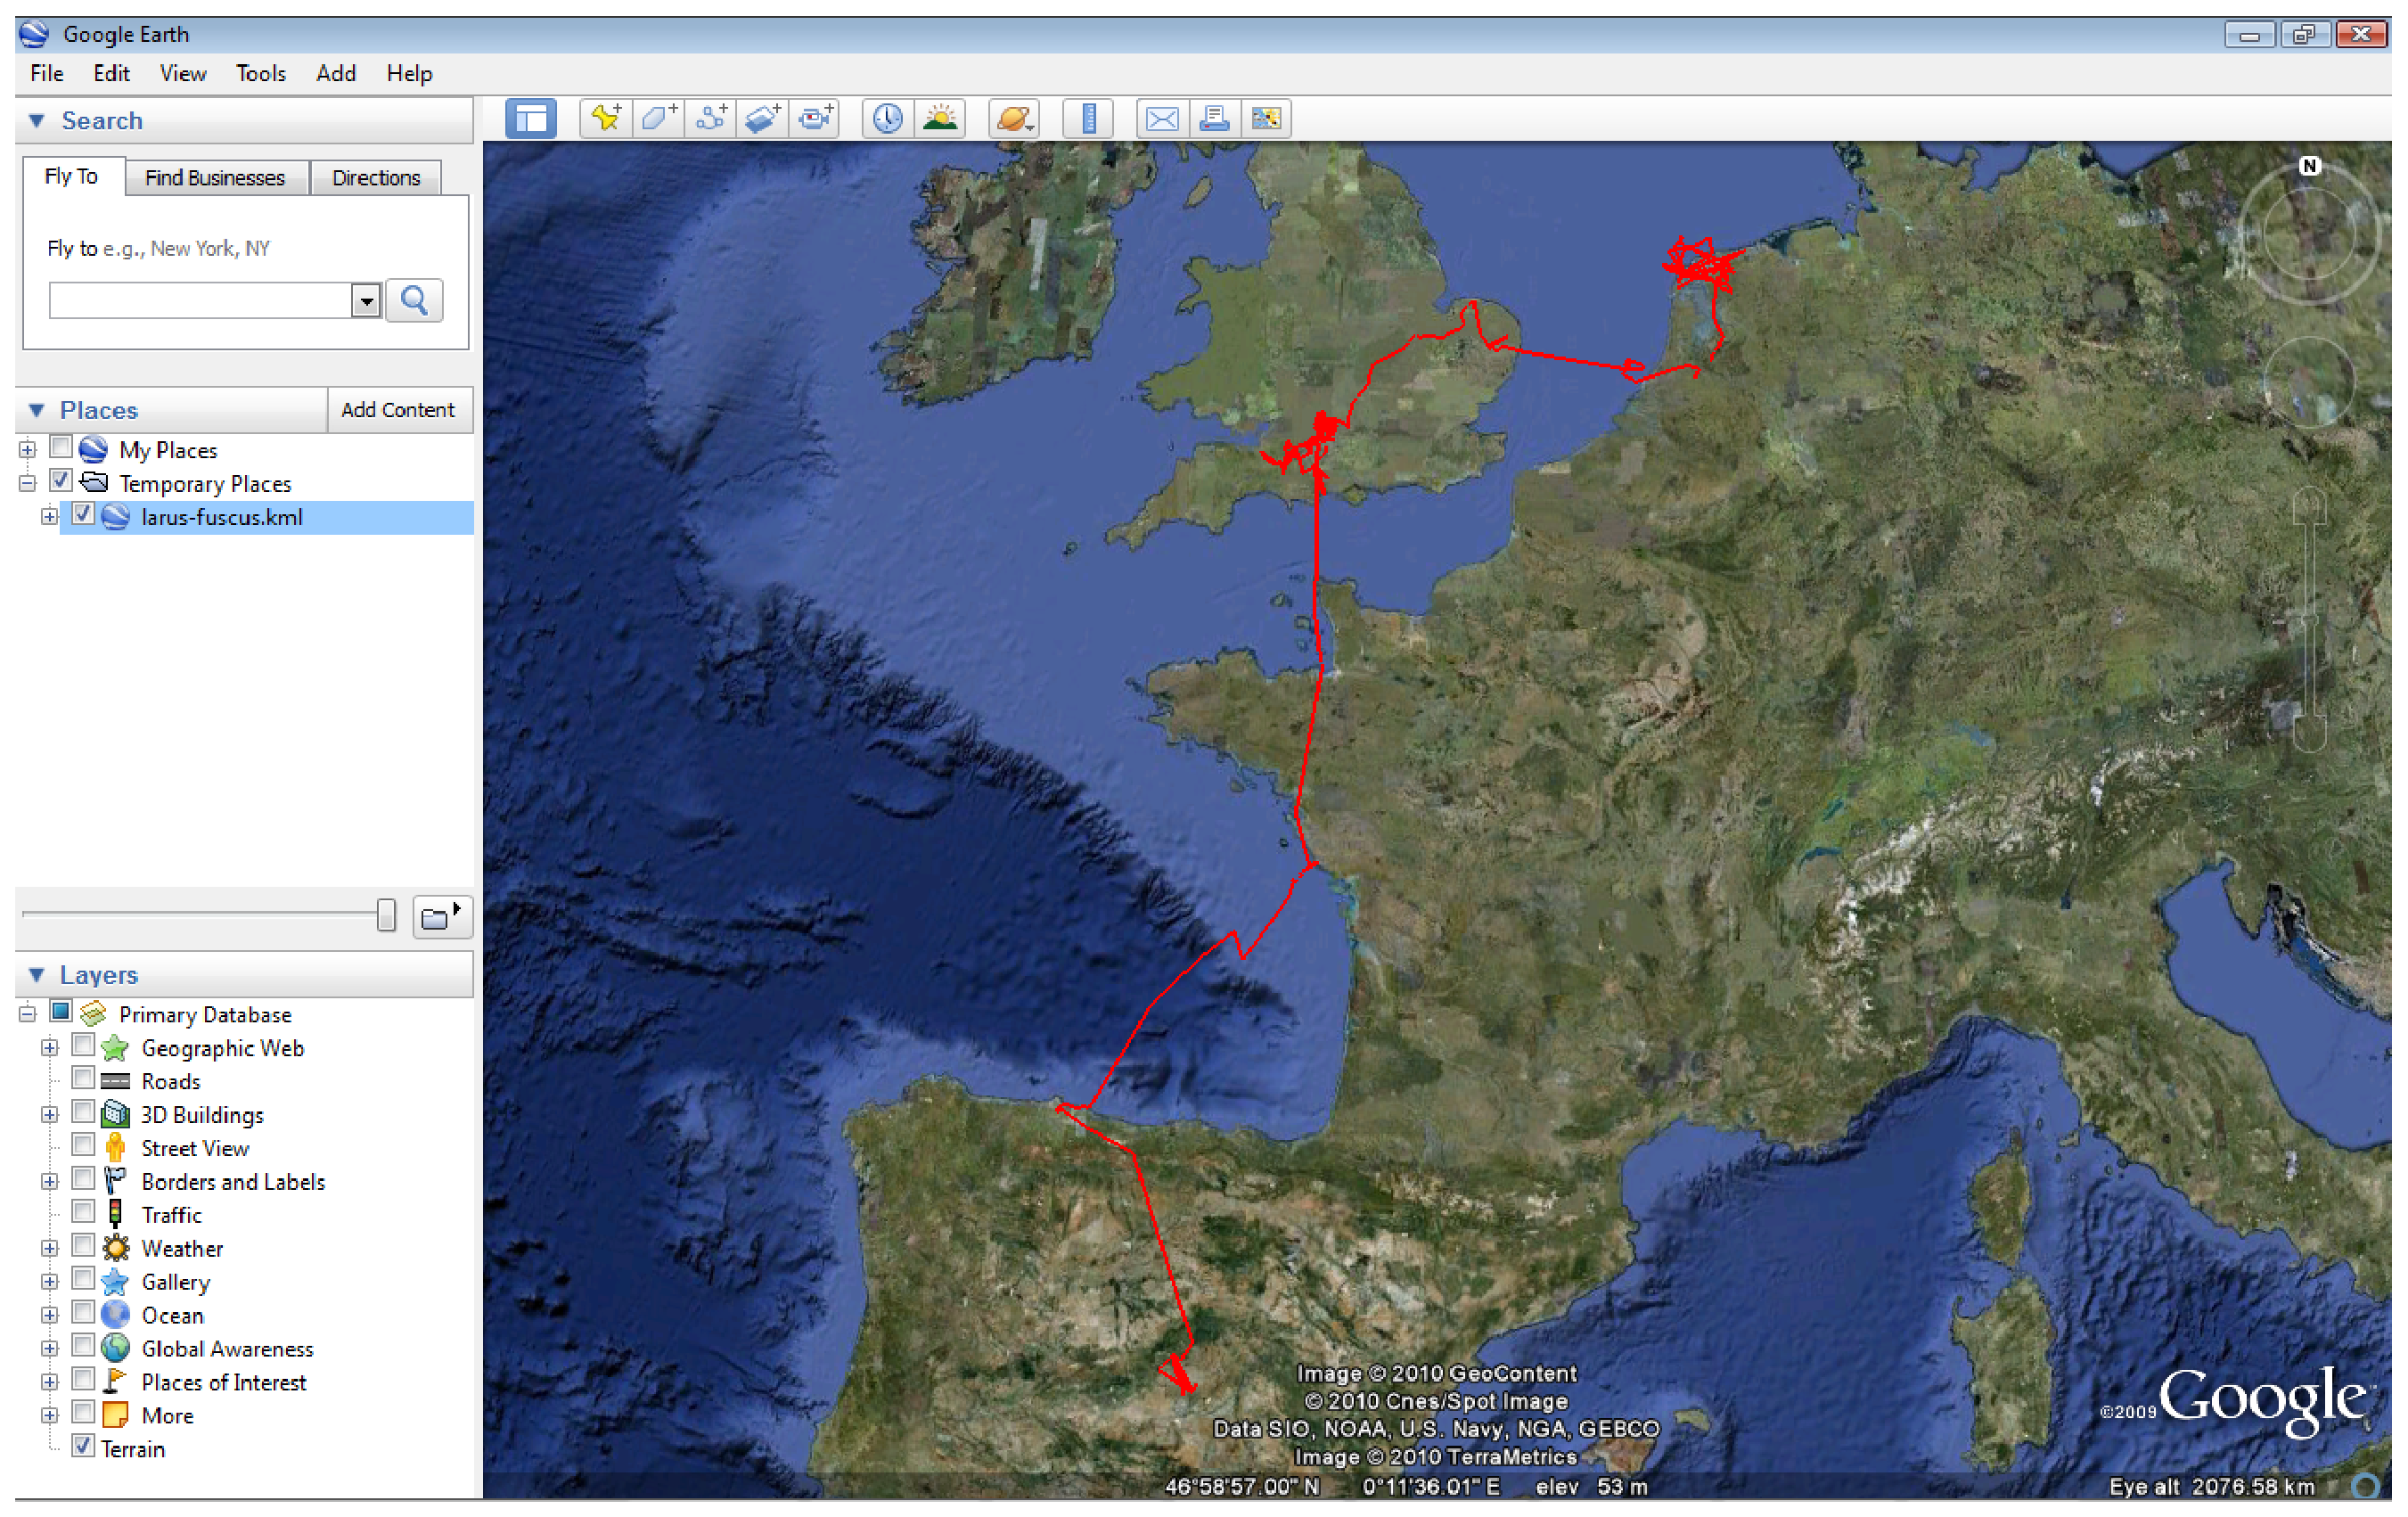
\includegraphics[width=1.0\textwidth]{./../eps/larus-fuscus.eps}}
  \caption{Bird track of seagull \#41745.}\label{fig:larus-fuscus}
\end{figure}

\begin{action}
Alter your script in such a way that it displays a point for each location where a measurement was taken. For this, you need to iterate over the locations, generate a {\tt ge\_point}, and concatenate the result with the KML-text that you already had. You can use any icon that you like (but \url{http://maps.google.com/mapfiles/kml/pal2/icon26.png} is a good option, especially when used in combination with the {\tt \squote{iconScale}}\index{`iconScale@\texttt{\squote{iconScale}}} and {\tt \squote{iconColor}}\index{`iconColor@\texttt{\squote{iconColor}}} options). If you open your *.kml file in the GoogleEarth Viewer, you should see the red line of Figure~\ref{fig:larus-fuscus}, as well as many points.
\end{action}

\noindent So far, you have generated KML files that contain objects which are static, i.e. they do not change with time. However, sometimes you want to present your data in a dynamic way, somewhat like a movie. The KML specification allows for the inclusion of objects which are visible only during a particular time interval. To make this work, the object in question (such as a point or a line) needs to be assigned a start time and an end time, between which it will be visible. The start and stop times need to be passed as character arrays using the option {\tt \squote{timeSpanStart}}\index{`timeSpanStart'@\texttt{\squote{timeSpanStart}}} and {\tt \squote{timeSpanStop}}\index{`timeSpanStop'@\texttt{\squote{timeSpanStop}}}. The character array should be formatted according to the following layout: {\tt 2008-01-05T22:00:00Z} , or 10 PM on the 5$^{th}$ of January 2008.

\begin{action}
Alter your {\tt textread} call in such a way that, in addition to the latitude and longitude, the time information is now also loaded into the workspace as two separate variables {\tt startDateTime} and {\tt endDateTime}.
\end{action}

\begin{action}
Use a {\tt for}-loop to iterate over all measurements. For each measurement, generate a KML string using {\tt ge\_point} with the timespan options. Concatenate and write to a *.kml file as before. When opened in the GoogleEarth Viewer, you should see a line representing the entire migratory route of the gull, as well as a point representing its location at a particular time. When played back, the point should move along the migratory route.
\end{action}

\hintbox{When the objects in the GoogleEarth Viewer are dynamic (i.e. when they have time labels), the upper left part of the main window contains additional controls with buttons for playback of the KML objects.}

\vspace{-2em}

\section{Rasterized imagery}
In the domain of Earth Sciences and Biology, we often have data in the form of maps. In this section, you will use the GoogleEarth Toolbox to visualize a map of Zinc concentrations in the Meuse river valley near Stein, The Netherlands. An array with spatial predictions of Zinc has already been derived from point measurements by means of a geostatistical method (ordinary kriging). This data is available as `pim\_files\textbackslash{}ch13\_toolboxes\textbackslash{}ok-predictions-radius.mat'.

\begin{action}
Start a new script `\starred{name}\_zinc.m'. Let it load the kriging data\footnote{Data from: Rikken, M.~G.~J. and Van Rijn, R.~P.~G. (1993) \textit{Soil pollution with heavy metals --An inquiry into spatial variation, cost of mapping and the risk evaluation of copper, cadmium, lead, and zinc in the floodplains of the Meuse west of Stein, the Netherlands.} Dept. of Physical Geography, Utrecht University} and visualize it using {\tt imagesc(pre)}. Include a title and a colorbar. 
\end{action}

\begin{action}
Consult the documentation on how to visualize raster-based images using {\tt ge\_imagesc}.
\end{action}


\noindent Table~\ref{tab:zinc-map-boundaries} contains the boundaries of the map. As you can see, they are given in degrees-minutes-seconds notation; for instance, the Northern border is at 50 degrees, 59 minutes, 31.20 seconds. Since a minute is 1/60 of a degree, and a second is 1/3600 of a degree, the top border is at 50.9920 decimal degrees. The toolbox only accepts latitudes and longitudes in decimal degrees. 
\begin{action}
You must write a function that converts degrees-minutes-seconds to decimal degrees. Start a new function m-file. Save it as `\starred{name}\_degminsec2decdeg'. The function should have 3 numerical input arguments (degrees, minutes and seconds), and one output argument (decimal degrees). Don't forget to include a comment help block.
\end{action}

\begin{table}[!ht]
\caption{Zinc map boundaries}
\label{tab:zinc-map-boundaries}
\vspace{-0.25em}
\centering
\begin{tabularx}{0.8\textwidth}{ |X|X| } \hline
\textbf{Boundary}&\textbf{Location}\\ \hline
North&50$^\circ$59\textquotesingle{}31.20\textquotesingle{}\textquotesingle{} \\ \hline
East&5$^\circ$46\textquotesingle{}11.40\textquotesingle{}\textquotesingle{} \\ \hline
South&50$^\circ$57\textquotesingle{}18.91\textquotesingle{}\textquotesingle{} \\ \hline
West&5$^\circ$43\textquotesingle{}13.36\textquotesingle{}\textquotesingle{} \\ \hline
\end{tabularx}
\end{table}


\begin{action}
For negative latitudes and longitudes, the function probably does not give the right result (-50$^{\circ}$59\textquotesingle{}31.2\textquotesingle{}\textquotesingle{} $\neq$ -49.0080$^{\circ}$). Alter your function in such a way that it first checks whether the input argument `degrees' is negative, and {\tt if} that is the case, make a slightly different calculation.
\end{action}

\begin{action}
Study \lstlistingname~\ref{list:example-ge_imagesc} (You can find a copy of this file in your work directory `pim\_files\textbackslash{}ch13\_toolboxes\textbackslash{}'). After studying the example m-file, use {\tt ge\_imagesc} to let your script generate a KML-formatted character array and have it written to disk.
\end{action}
\lstinputlisting[float=htbp,caption={Contents of the file `example\_ge\_imagesc.m'},label=list:example-ge_imagesc]{./../m/example_ge_imagesc.m}
\begin{action}
Open your *.kml file in the GoogleEarth Viewer and verify that it is displayed correctly. 
\end{action}
\begin{action}
Consult the documentation on {\tt ge\_colorbar}\index{ge\_colorbar@\texttt{ge\_colorbar}}. Let your script generate the KML-formatted text that contains the colorbar information. Concatenate the 2 KML character arrays and pass them to {\tt ge\_output}.
\end{action}
\begin{action}
Go back to the GoogleEarth Viewer, and right-click on the name of your object. Select \guitext{Revert} to let GoogleEarth reload the file. Check that a colorbar is now included in the file.
\end{action}
\begin{action}
By default, the colorbar is labeled `ge\_colorbar' when displayed in the GoogleEarth Viewer. Change it to a more descriptive name.
\end{action}

\begin{action}
What is the lowest value in {\tt pre}? This value is used to determine the range of colors, even though the map does not contain any concentrations below 119.368 ppm. As a result of the stretched-out colorbar, there is not enough color differentiation in the research area. Let your script remedy this by setting the color limits explicitly.\index{`\squote{cLimLow}@\texttt{\squote{cLimLow}}}\index{`\squote{cLimHigh}@\texttt{\squote{cLimHigh}}}
\end{action}

\begin{action}
In the GoogleEarth Viewer, verify that the colors on the colorbar no longer correspond with those that are displayed. Change your script in such a way that the color limits are also applied to the colorbar.
\end{action}

\begin{action}
The array {\tt pre} contains -1 values where the kriging method has not been applied. Using {\tt ge\_imagesc}'s option {\tt \squote{alphaMatrix}}\index{`\squote{alphaMatrix}@\texttt{\squote{alphaMatrix}}}, you can specify for each element in {\tt pre} how transparent it should be. Use relational operators to make an array {\tt transpArray} that contains the transparency\index{transparency} information. Consult the documentation on the option {\tt \squote{alphaMatrix}} to make the area surrounding the research area 80\% transparent.
\end{action}

\begin{action}
Make the research area itself 20\% transparent.
\end{action}





\vspace{1em}
\noindent If you have executed all the exercises correctly, your *.kml file should look like Figure~\ref{fig:zinc-stein}.

\begin{figure}[!htbp]
  \centering
    \fbox{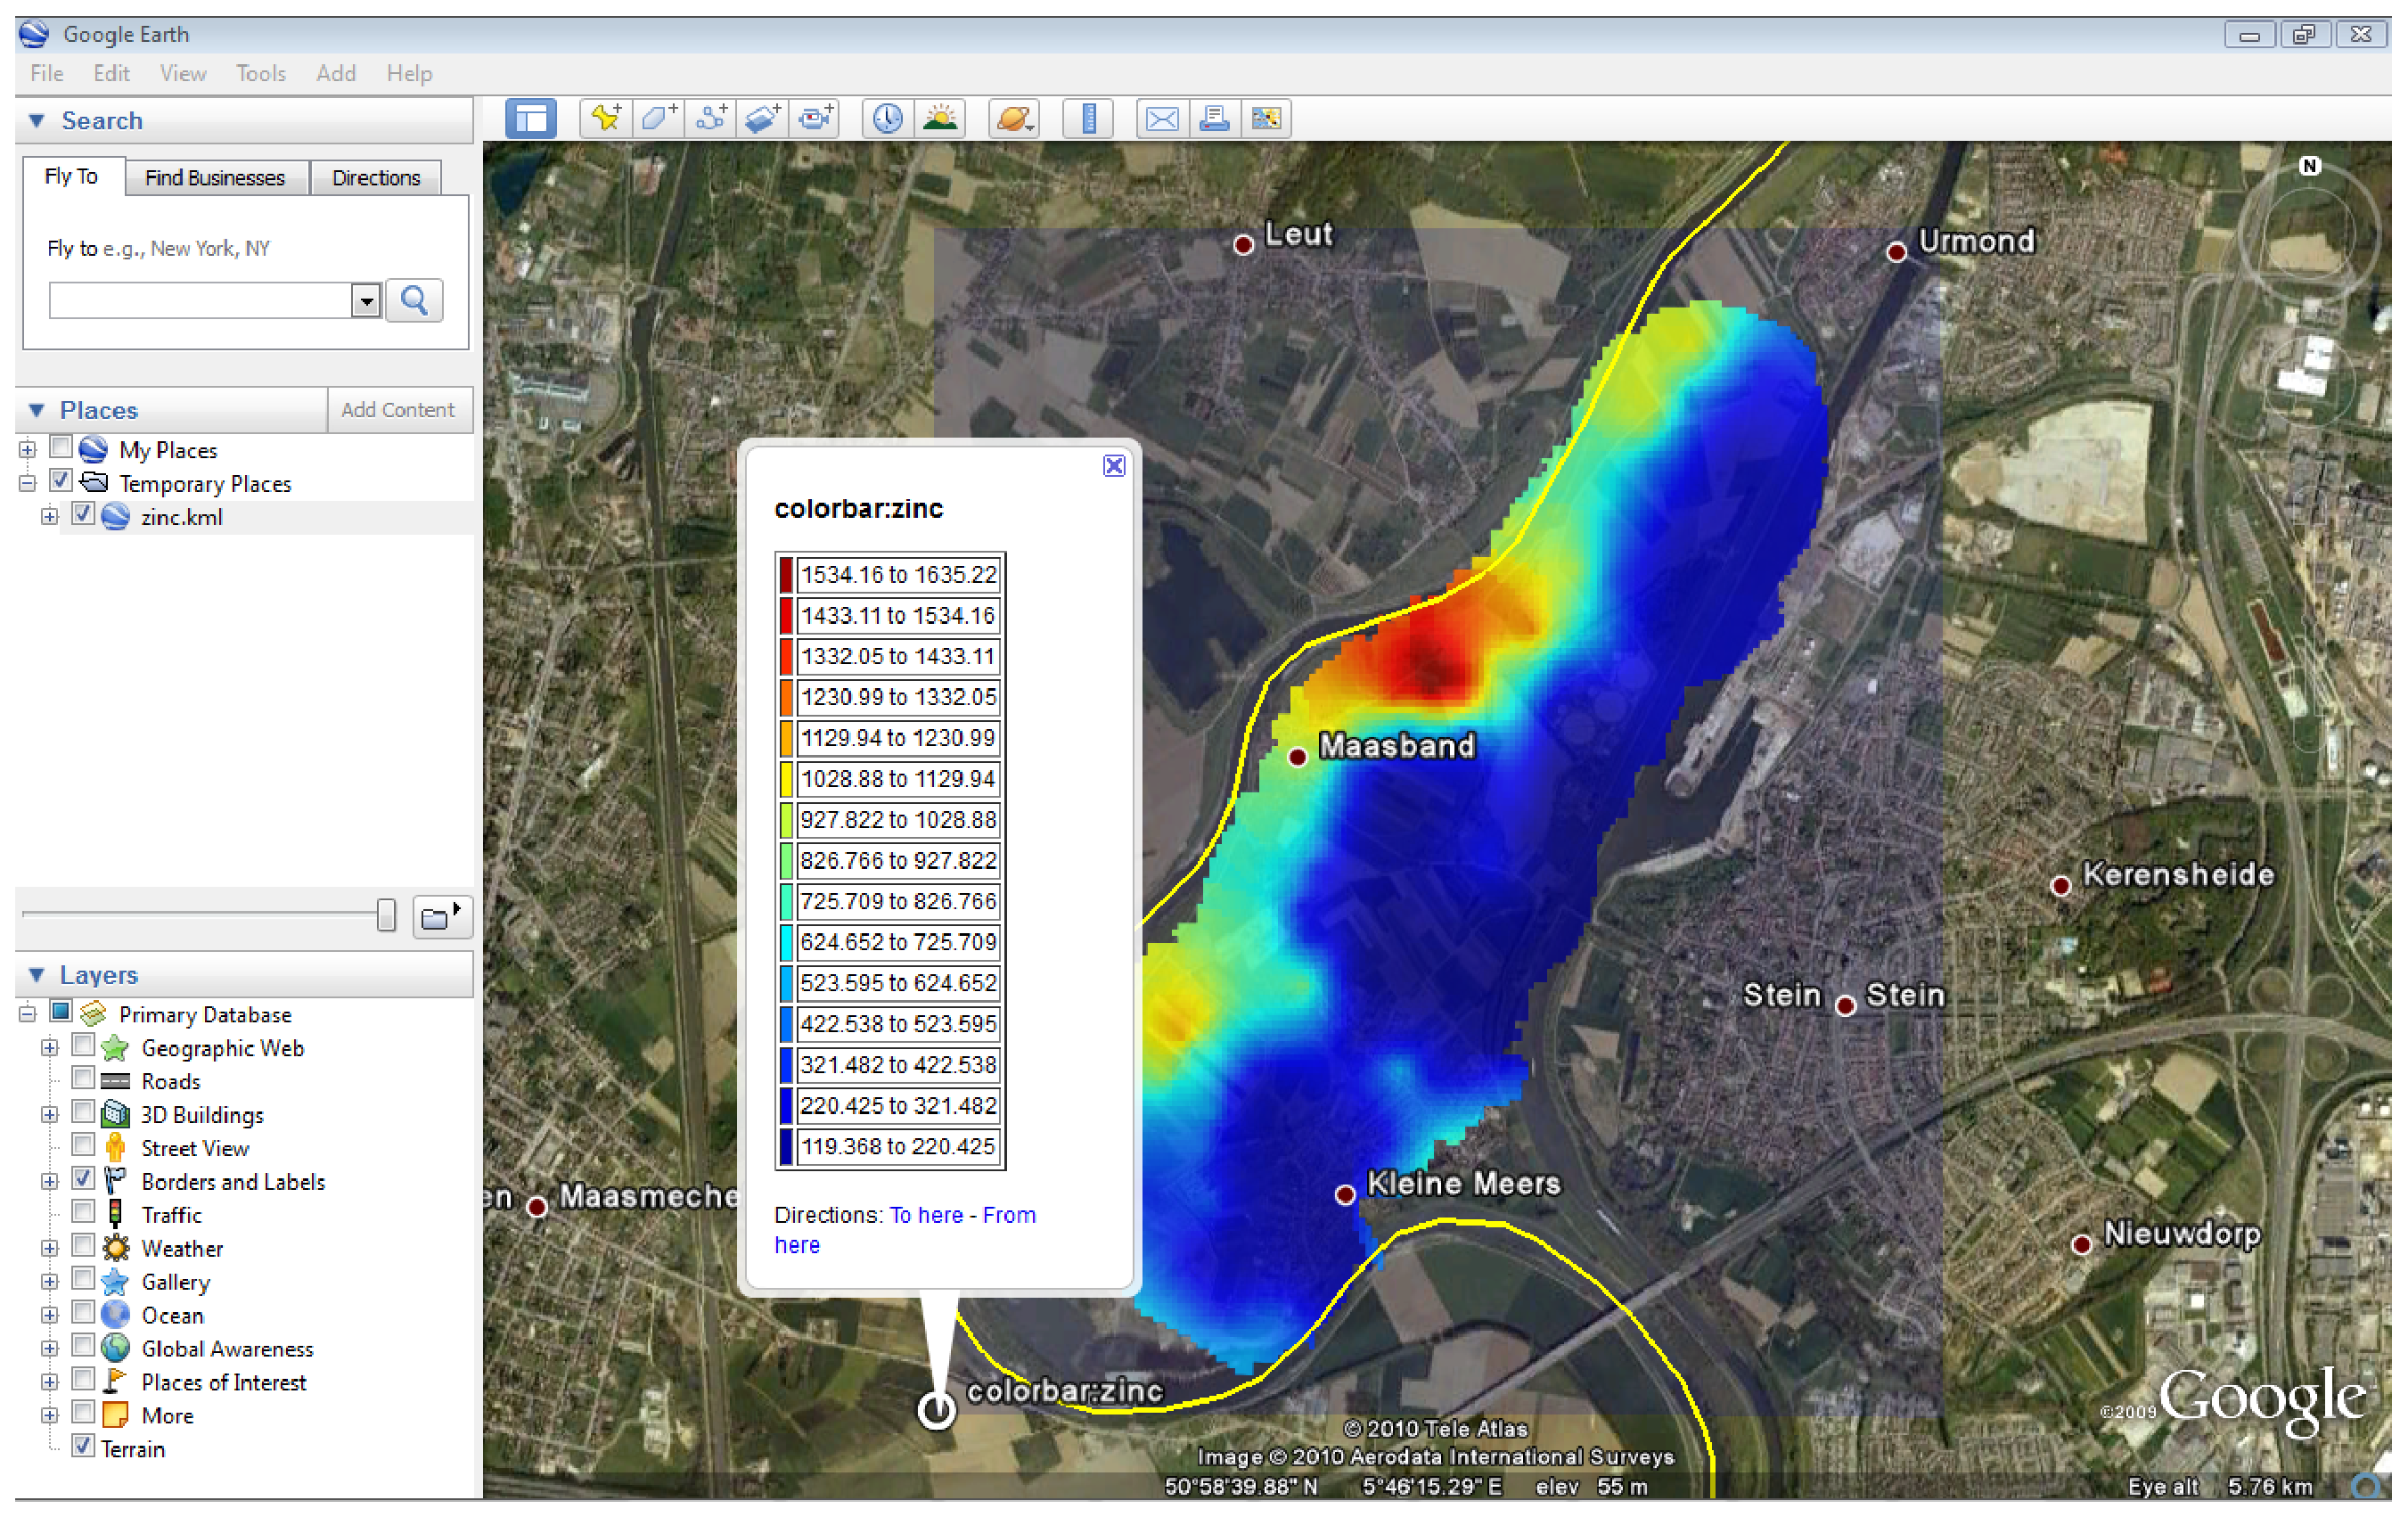
\includegraphics[width=1.0\textwidth]{./../eps/zinc-stein.eps}}
  \caption{Zinc concentrations near Stein}\label{fig:zinc-stein}
\end{figure}



%\section{Advanced features}
%
%\subsection{Time-variant features}
%In addition to displaying static features, the GoogleEarth Viewer can also visualize dynamic content. 
%
%

%\subsection{Filled contour plots}


\projectfooter




\backmatter
%\chapter{Extra projects}
\thispagestyle{fancy}
\label{ch:extra-projects}


%\chapter{Exam}
\thispagestyle{fancy}
\label{ch:example-exam}

\printindex
%\insertemptypage{}

\end{document}